% some definitions for the title page
\newcommand{\reporttitle}{PhishingLine: Hybrid Phishing Classifier with Logo Detection}
\newcommand{\reportauthor}{Kabeer Vohra}
\newcommand{\supervisor}{Dr. Sergio Maffeis}
\newcommand{\secondmarker}{Dr. Luis Mu\~noz-Gonz\'alez}
\newcommand{\reporttype}{Individual Project Final Report}
\newcommand{\degreetype}{Computing Masters of Engineering degree} 

\documentclass[12pt,twoside]{report}
\usepackage[utf8]{inputenc}
\usepackage[margin=1.2in]{geometry}
\renewcommand{\baselinestretch}{1.4}
\newcommand{\powerset}{\raisebox{.15\baselineskip}{\Large\ensuremath{\wp}}}
\usepackage{multirow,array,graphicx,amsmath,epigraph,amsfonts,enumitem,easytable}
\PassOptionsToPackage{hyphens}{url}\usepackage{hyperref}
\setcounter{tocdepth}{4}
\setcounter{secnumdepth}{4}
\usepackage{titlesec}
\titleformat{\chapter}
  {\normalfont\LARGE\bfseries}{\thechapter}{1em}{}
\titlespacing*{\chapter}{0pt}{3.5ex plus 1ex minus .2ex}{2.3ex plus .2ex}
\newpagestyle{mystyle}
{\sethead[\thepage][][\chaptertitle]{}{}{\thepage}}
\pagestyle{mystyle}
\usepackage[backend=biber]{biblatex}
\addbibresource{bibliography.bib}
\usepackage{tablefootnote}
\usepackage{longtable}
\usepackage{array}
\usepackage{makecell}
\usepackage{appendix}
\usepackage{fancyvrb}
\usepackage{setspace}
\usepackage[format=plain,font=it]{caption}
\usepackage[T1]{fontenc}

\setlength\epigraphwidth{16cm}
\setlength\epigraphrule{0pt}

\usepackage{etoolbox}

\makeatletter
\patchcmd{\epigraph}{\@epitext{#1}}{\itshape\@epitext{#1}}{}{}
\makeatother

\title{}
\author{Kabeer Vohra}


\begin{document}
% Last modification: 2015-08-17 (Marc Deisenroth)
\begin{titlepage}

\newcommand{\HRule}{\rule{\linewidth}{0.5mm}} % Defines a new command for the horizontal lines, change thickness here

%----------------------------------------------------------------------------------------
%	LOGO SECTION
%----------------------------------------------------------------------------------------


\includegraphics[width = 4cm]{./images/imperial}\\[0.5cm] 

\center % Center everything on the page
 
%----------------------------------------------------------------------------------------
%	HEADING SECTIONS
%----------------------------------------------------------------------------------------

\textsc{\LARGE \reporttype}\\[1.5cm] 
\textsc{\Large Department of Computing}\\[0.5cm] 
\textsc{\large Imperial College of Science, Technology and Medicine}\\[0.5cm] 

%----------------------------------------------------------------------------------------
%	TITLE SECTION
%----------------------------------------------------------------------------------------

\HRule \\[0.4cm]
{ \huge \bfseries \reporttitle}\\ % Title of your document
\HRule \\[1.5cm]
 
%----------------------------------------------------------------------------------------
%	AUTHOR SECTION
%----------------------------------------------------------------------------------------

\begin{minipage}{0.4\textwidth}
\begin{flushleft} \large
\emph{Author:}\\
\reportauthor % Your name
\end{flushleft}
\end{minipage}
~
\begin{minipage}{0.4\textwidth}
\begin{flushright} \large
\emph{Supervisor:} \\
\supervisor \\ % Supervisor's Name
\emph{Second Marker:} \\
\secondmarker % Supervisor's Name
\end{flushright}
\end{minipage}\\[4cm]




%----------------------------------------------------------------------------------------


%----------------------------------------------------------------------------------------
%	DATE SECTION
%----------------------------------------------------------------------------------------

{\large \today} % Date, change the \today to a set date if you want to be precise


\vfill % Fill the rest of the page with whitespace
Submitted in partial fulfillment of the requirements for the \degreetype~of Imperial College London

\end{titlepage}

\pagenumbering{roman}
\shipout\null
%%%%%%%%%%%%%%%%%%%%%%%%%%%%%%%%%%%%
\begin{abstract}
Phishing attacks are one of the most lucrative forms of online fraud today. In these attacks, criminals lure victims into disclosing sensitive information by masquerading as another legitimate entity. Unlike traditional malware, which typically is automatically detected by local anti-virus software, phishing attacks are online and therefore need to be identified and blacklisted. The sheer volume and rapidity with which phishing pages are created, requires that browsers need to update from popular blacklists, such as Google Safe Browsing, every five minutes in order to keep users reasonably well protected.
\\\\
Recent research has identified machine learning as an effective way to improve automated phishing detection.
In this report we present our hybrid classifier, a novel approach which combines analysis of page attributes with cascading classifiers on extracted images and screenshots.
\\\\
We have developed a platform which performs comparably with the current state of the art, whilst detecting pages with the equivalent of research leading performance, and providing an easily extensible platform for future collaborators. Additionally, our learning platform is designed to be able to automatically adapt to new styles of malicious pages and fit to new phishing techniques.
\end{abstract}

\clearpage{\pagestyle{empty}\cleardoublepage}
%%%%%%%%%%%%%%%%%%%%%%%%%%%%%%%%%%%%
\newgeometry{margin=1in}
\chapter*{Acknowledgments}
I would like express my gratitude to my supervisor, Dr. Sergio Maffeis, thank you for all your helpful feedback and guidance in our regular meetings as well as being available on slack most hours of the day.
\\\\
I would also like to thank my second marker, Dr Luis Muñoz-González for assisting me on the machine learning parts of the project and being available for meetings at a moments notice.
\\\\
To Marco, Clemens, Guillherme, Alessandro and everyone else at Lastline. Thank you for all the help, allowing me to work from your office, regular meetings and providing me with all the data and structure to complete this project.
\\\\
To Dad, my best mate. Thank you for all you have given me throughout my entire life and all the football and music we have shared.
\\\\
To Mum. Thank you for all of the guidance and counselling you have given me, our regular nights out together are always special.
\\\\
To Aneet and Neha. Thank you for all the laughs and fights we have had in equal proportion over the past 19 years.
\\\\
To Clelia. Thank you for dealing with all my moaning over the past year, there's more to come.
\\\\
To Gaurav, David, Chinmay, Elyas, Florian, Mahir, Jack, Harry, Nihal and all my other friends over the course of this degree. Thank you for all your help and all the good times we shared.
\restoregeometry
\clearpage{\pagestyle{empty}\cleardoublepage}
\setcounter{page}{1}
\tableofcontents
\newpage
\pagenumbering{arabic}
\chapter{Introduction}
\textbf{Social engineering} is the art of hacking the human psyche. The victim is tricked into divulging confidential information or to perform specific actions. It is not merely a modern phenomenon, for time immemorial people have used this method to gain access to resources the victim may have. Recently, Michael Wolff `scooped' the world's journalists when he was able to gain permission to be a fly-on-the-wall inside the White House simply by using basic strategies of social engineering. This allowed him to write one of the first books about the Donald Trump presidency~\cite{whitehouse}.
\\\\
With the advent of the digital era, and the omnipresence of the internet in today's society, criminals have realised how easy it is to move this practice online and weaponise their efforts. This practice is known as \textbf{phishing}.
Criminals can use this illicitly collected data to steal money, perform identity fraud or even to make physical attacks using obtained home addresses.
\\\\
Phishing attacks will often initially masquerade in the form of an email alerting the victim that something is wrong, thereby creating a sense of urgency. This may result in users performing actions, without taking due care that the email is legitimate. Common elements of such emails include logos of target websites, language to create a sense of urgency and a link to the phishing website. An example phishing email can be found in figure \ref{fig:phishingemail}.
\\\\
Unlike many elements of cyber security which are a constant arms race between researchers and attackers, 90\% of phishing attacks examined over the 10 months between late 2016 and mid 2017 were replicas of attacks already detected~\cite{phishingovertime}. Whilst we are able to roll out patches for known security flaws swiftly, the size and nature of the internet makes phishing a much harder problem to tackle.
\\
\begin{figure}[!h]
  \begin{center}
    \fbox{
\includegraphics[width=0.8\textwidth]{images/phishingemail.png}}
  \end{center}
  \caption{Example phishing email received advertising fake prize in order to gain access to Amazon login credentials}
  \label{fig:phishingemail}
\end{figure}
\section{Motivation}\label{motivation}
Various methods of classification in the literature today have different benefits. Cantina had an extremely high true positive rate but also suffered from many false positives~\cite{cantina}. Whittaker et al. had similar issues with their methods of classifying pages using PageRank~\cite{largescaleautomatic}. All the phishing pages they investigated had a very low PageRank, however this was true for many legitimate pages as well. For this reason a hybrid approach has been used in more recent techniques, where classifiers can use a combination of the most effective approaches to gain the highest sensitivity and specificity. 
\\\\
Creating a modular solution allows us to implement different methods and combine the results of these independent classifiers. In this way we have the ability to easily extend the classifier by creating further modules and consistently improving the accuracy of the classifier.
\\\\
Often in phishing attacks, criminals may choose to imitate the brand rather than simply creating clones of legitimate pages. Whilst these pages may not have any visual similarity with pages on the target domain, they will need to include the branding of the target company. Without this branding, it would be difficult to convince the victim that they are visiting a page originating from the target brand. By detecting this on the page, we would then be able to check if this page actually resides on the domain of the brand, or elsewhere. We also know that, according to the anti-phishing working group, in Q4 of 2017 there were a total of 640 unique brands targeted and a few hundred companies attacked regularly~\cite{apwg}. For this reason it should be feasible to be able to gather the data for all of these targets using a script and then use this data to try and identify the target brands.
\\\\
Phishing pages today are mostly created using phishing kits. These kits allow the attacker to quickly generate fully-fledged phishing pages, ready to be deployed. According to Marco Cova et al., newly detected phishing kits are often derivatives of previous kits that are still currently active~\cite{freephish}. Therefore it is self-evident that the HTML provided by these kits will be similar to previously detected kits and the same will be true of the phishing pages which use these kits. From this assumption we can try and compare the DOM trees pages which we wish to classify with known phishing pages as a metric to evaluate if we believe the page is using a derivative of the kits which we have discovered.
\\\\
In order to compare DOM trees, it is interesting to try and compute bi-simulations between them. To do this, we can take pairings between the two DOM trees, and then use a fitness function to compute which pairs we wish to keep, and which we want to ignore. By applying a progressive monotonic function, we are able to reduce the obtained set, and then use this data to compute a metric on the similarity of the two pages.
\section{Contributions}
In this report we developed a hybrid machine learning based approach to phishing classification. We will summarise the main modules of our final pipeline here.
\begin{itemize}
    \item \textbf{URL (Section \ref{urlvectorizer}): }We analyse the URL for many of the common features that attackers may use in order to trick the victim into trusting the page. The URL provided some of the most important features in our overall classifier and can be useful to use as a single module if we wanted to prioritise performance only.
    \item \textbf{Word Frequency (Section \ref{wordfrequencyvectorizer}): }Our word frequency module allows us to analyse the direct textual content on the pages for the highest frequency. Often, phishing websites use similar terminology and therefore we can automatically learn these words as the pages evolve.
    \item \textbf{HTML (Section \ref{htmlvectorizer}): }In this module we extract features in order to profile the structure of the page to feed into our classifier. We attempted to compute the DOM similarity between phishing pages but found it difficult to do effectively with the structure of our classifier.
    \item \textbf{Page Resources (Section \ref{resourcevectorizer}): }We analysed the locations of the resources that the page loaded in as well as where the page sent data. Often phishing pages need to load resources from other hosting sources or directly from the page which they are trying to imitate. They will also need to exfiltrate the stolen credentials to their servers which may be different to the ones on which the page is hosted.
    \item \textbf{Logo Detection (Sections \ref{screenshotvectorizer} and \ref{imageresourcesvectorizer}): }When trying to determine the brand of a page, phishing websites use familiar logos to trick victims visiting the page. We use various computer vision techniques to detect the logo on the page and then subsequently determine whether the page originates from the source corresponding to the logo.
\end{itemize}

\chapter{Evaluation Techniques}
In the following chapters of this report we will present our classifier and other approaches in the literature which have been evaluated using some of the techniques below.
\section{Sensitivity and Specificity}
Classification algorithms are measured by their \textit{sensitivity} and \textit{specificity}.
\\\\
The sensitivity of a test is judged by its \textit{true positive rate}. This is the proportion of websites which are phishing sites and have been classified as such. A highly sensitive test is one that classifies most of the phishing sites correctly. An example of which is Cantina developed by Y. Zhang et al~\cite{cantina}.
\\\\
With a highly sensitive test we can be quite certain that if the test classified the webpage as benign (non-phishing), then it would be a correct judgement. We would not be confident, however, that if the test marked a page as phishing, whether it was correct or if the page was a benign page.
\\\\
The specificity of a test is judged by its true negative rate. This is simply the legitimate websites that have not been classed as phishing. If we have a high true positive and high true negative rate, then we would have a good classifier.
\\\\
Conversely, false positive and false negative results are where the test incorrectly classifies the data as a phishing site or a non-phishing site respectively.
\\
\clearpage
\section{Confusion Matrix}
A confusion matrix is a table which allows us to classify our results into true positive, true negative, false positive and false negative.
\begin{table}[h]
\begin{center}
\begin{tabular}{l|l|c|c|c}
\multicolumn{2}{c}{}&\multicolumn{2}{c}{True classification}&\\
\cline{3-4}
\multicolumn{2}{c|}{}&Non-phishing&Phishing\\
\cline{2-4}
\multirow{2}{*}{Test result}& Non-phishing & $TN$ & $FP$\\
\cline{2-4}
& Phishing & $FN$ & $TP$\\
\cline{2-4}
\end{tabular}
\end{center}
\caption{An example confusion matrix}
\label{table:confusionmatrix}
\end{table}
\section{Complementary Cumulative Distributions}
Complementary Cumulative Distributions (CCDF) are used in order to show what percentage of the data set is above a certain threshold. An example can be seen in figure \ref{fig:pagerankphishing}. Here we can see that there are no phishing pages with PageRank above 0.5 since the graph intersects with the x-axis at this point.
\section{Binary and Multiclass}
When classifying a page we can use either a binary or a multiclass classifier:
\\\\
\textbf{Binary} classifiers will output a single result as to whether the page is phishing or non-phishing.
\\\\
\textbf{Multiclass} classifiers can provide a set of output metrics which can then allow us to assess whether the page is phishing or not.
\section{ROC Curves}
ROC curves are common tools in binary classification. They allow us to evaluate what true positive rate we can achieve when considering the highest false positive rate that we can accept. Analysis of the ROC curves provide us with information to select optimal thresholds for the problem we have, dependent on whether we care, more about false positives or false negatives. Lines on the ROC curve that fall below the dotted line are considered to be worse than simply selecting a random classification with a success rate of 50\%.

\section{Cross-Validation}
Overfitting is a common problem within machine learning techniques. It is where the classifier can start learning the selection bias which we have within our data set which will not help us to classify new examples very well. Generalizability is important in trained models and overfitting kills this. Our initial testing may seem positive but we need methods to ensure that we are accurately evaluating our classifier so that when it is fed new data it is still able to classify correctly.
\\\\
To solve this problem we use k-fold cross validation, this is a technique used to split the training data into $k$ separate splits and then use $k-1$ splits to train and one to test, we repeat this $k$ times with the single test subset rotating among the $k$ subsets. This allows us to ensure that the entire test set can be correctly classified and that our classifier is not over fit to a single test set.
\newpage
\chapter{Current State of Phishing}
\section{Primarily Affected Industries}
According to the anti-phishing working group, the top 3 targets for phishing attacks in the second half of 2017 were payment, financial institutions and webmail~\cite{apwg}.
\subsection{Payment}
The payment industry makes up 42\% of all phishing attacks. Easy access to victim’s money is the obvious driver for this high metric. Typically smaller payment services have less sophisticated anti-fraud departments than do the banking industry, making them easier targets for potential attacks.
\subsection{Financial}
Whilst these companies typically have sophisticated anti-fraud protections in place, financial institutions still make up 15\% of all attacks, criminals realise that the most lucrative method is still to go directly to the banks. With the rise of Bitcoin and other anonymised decentralised currency systems, it is becoming much harder for institutions to protect users’ money and reverse fraudulent transactions~\cite{bitcoin}.
\\\\
Online banking services often implement phishing prevention best practices in order to warn the user if they are not on the legitimate site. Santander for example implement the recognised image technique where they assign an image to the user to be displayed before they login. If the user reaches a login page without the image this should hopefully arouse suspicion. 
\subsection{Webmail}
Exploiting a user's webmail account gives access to all online login details associated with that email address. Due to this expanded benefit, fraudulent webmail access is highly valuable and makes up 16\% of the overall market.
\section{Attack Characteristics}
\subsection{Lifetime}
Phishing attacks are generally alive for a very short period of time before they are rendered useless. The lifespan of an attack is measured as the time between the first and last observed attack instance.
\\\\
In the research conducted by Qian Cui et al. 34\% of phishing attacks only last between 1-7 days after they were made active, longer attack classes can last between 2 and 10 months~\cite{phishingovertime}. The average time for an attack class to be active is 25 days.
\\\\
Although these attacks are closed down so quickly, they clearly still remain extremely lucrative. Attackers generally set many attacks at once and profit during the short window of opportunity that the phishing attacks are active.
\subsection{Phishing Kits}
Phishing kits are very popular in the phishing world today, they allow would-be criminals to create phishing exploits with little technical skill. These kits are usually sold anonymously on the dark web by malicious developers through the use of Bitcoin and other untraceable cryptocurrencies~\cite{bitcoin}.
\\\\
The kits vary in technical complexity, they can be very basic pages which mimic the brand and have no credential verification\footnote{Credential verification is when the phishing website ensures the input details are valid against the legitimate website before letting the user proceed}; or they can be more complex attacks which are virtually indistinguishable from the legitimate page and perform validation against a real API to ensure the credentials are valid.
\\\\
Analysis of a more sophisticated kit by ProofPoint, aimed at PayPal, showed that form validation was done only on the username field by using a deprecated API provided by PayPal themselves~\cite{proofpoint}.
\\\\
After the user proceeds to login, the kit also asks the user to confirm bank credentials to secure their account, all this information is logged in the backend portal of the phishing kit. This particular phishing kit also allows for a `selfie mode' which allows the attacker to access the webcam of the victim as well.
\subsection{PHP}
Marco Cova et al. used various methods in order to obtain phishing kits that are being used today~\cite{freephish}. Each of the 584 kits obtained were written in PHP. PHP is a popular language because it is widely supported and enabled on most web servers.
\\\\
The use of PHP was leveraged in the implementation of the PhishEye honeypot~\cite{phisheye}. Two Apache HTTP modules \texttt{mod\_php} and \texttt{mod\_security} were extended in order to track actions that were taken in the PHP exploits.
\\\\
From \textbf{mod\_php} they modified three handlers, \texttt{rfc1867\_post\_handler}, \texttt{php\_std\_post\_handler} and \texttt{php\_default\_treat\_data}. These three handlers deal with any form posts, POST and GET requests. All of these were recorded along with the IP address of the caller.
\\\\
\textbf{mod\_security} was used in order to perform data mangling so that the criminal would not receive any sensitive information.
\subsection{URL Obfuscation} \label{urlobfuscation}
For attacks which are not hosted on the target page, attackers generally use four different techniques in order to obfuscate the illegitimacy of the URL from the user~\cite{freephish}.
\\\\
\textbf{Technique I} is to purchase commonly misspelt domains and host them as phishing websites. With this technique the URL seems legitimate, since it is virtually identical to the target URL. Apart from the redirection benefits, say from an email, the hacker is also able to serendipitously capture victims who have simply mistyped the URL themselves. An example of this could be \url{https://gooogle.com}. Whilst large organisations usually purchase most of the commonly misspelt URLs, this can be an effective method for second tier company websites. 
\\\\
\textbf{Technique II} is to purchase a short domain and have the full correct URL prepended to this short name. An example of this could be \url{https://bank.barclays.com.vit.ly}. This methodology is the most effective if the target domain is secure and there are no obviously misspelt domains available.
\\\\
\textbf{Technique III} is when the attacker compromises another domain which has a backdoor and hosts the attack on there. The backdoor URL will contain the name of the target of the attack, for example \url{https://compromiseddomain.com/barclays}. This method provides a lower overhead for the attacker since they do not need to register a separate domain themselves. It also reduces the risk they take of being caught from information related to the registration of the domain they use for the attack.
\\\\
\textbf{Technique IV} is when the domain has absolutely no relation to the target of the attack. These are the least effective methods but also have the lowest overhead. For these attacks, the criminal needs only to find a domain which has a backdoor and uses this to host their attacks.
\\\\
It is important to note that using HTTP Secure protocol (HTTPS) is a very effective tactic that is used. By displaying the secure lock in the browser due to a valid SSL certificate, attackers are able to maintain a level of trust without deep inspection of the URL itself by the victim~\cite{https}.
\subsection{Data Exfiltration}
During phishing attacks, data exfiltration is a key issue for criminals. Either they can have the data written to a log and stored on the server which they can then retrieve or they need to have the data sent over email to an account that they use to collect the results.
\\\\
Email exfiltration is easier to detect by monitoring the outgoing SMTP and also contains the email address of the attacker. It is, however, preferred by some attackers because it avoids the need to have to re-access the compromised server to retrieve the data. This server may be patched or being monitored if the phishing kit has been detected. 

\subsection{PageRank}
PageRank is the algorithm that Google uses in order to determine which websites will be prioritised in their search results. It is a constantly evolving system which continually improves the quality of the results, and counteracts organisations which attempt to artificially promote their websites to the top.
\\\\
The algorithm is based, amongst other variables, upon the number of quality links from other reputable sources a website may have; in order to determine its importance as a website and provide legitimacy. Due to the short typical lifespan of an attack, the return on investment associated with improving PageRank for a specific malicious page is too low to justify the efforts required.
\\\\
As seen in Figure \ref{fig:pagerankphishing} by Colin Whittaker et al. none of the phishing pages have a high PageRank attribute\cite{largescaleautomatic}. This is a good classifier for the detection of phishing pages but, by itself, will also contain many false positives, due to the large quantity of legitimate pages which also have a low PageRank.
\begin{figure}[h]
  \begin{center}
    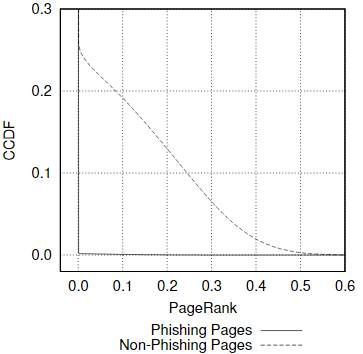
\includegraphics[width=0.5\linewidth]{images/pagerankphishing.png}
  \end{center}
  \caption{CCDF of PageRank for phishing and non-phishing pages~\cite{largescaleautomatic}}
  \label{fig:pagerankphishing}
\end{figure}
\section{Defence Mechanisms}
\subsection{Browser Extensions}
A study conducted by Y. Zhang et al. from Carnegie Mellon University evaluated many different anti-phishing toolbars~\cite{phindingphish}. These approaches all used a level of pre-processing before the page loaded and then displayed the level of risk associated with each page visited in a toolbar on the browser. Many methods were employed by these extensions such as investigating the source of the hosting with each page, using heuristics on the layouts of the pages, and comparing them against blacklist data.
\subsection{Blacklists}
Blacklists are lists of URLs which have been flagged as being malicious, these are generally inbuilt into the browser and the legitimacy of pages are checked before they are visited. With the rise in use of mobile phones, many of their browsers ban the use of extensions, therefore promoting the use of blacklists. In addition, the extra load time overhead of pre-processing the page before display makes inbuilt browser page blacklisting the approach that current researchers use.
\\\\
There are a wide range of methods that are employed today to improve classification of phishing websites in order to keep the blacklists updated frequently enough. Due to their monopolistic nature, Google is able to keep updated crawls of new pages across the internet to refresh their Safe Browsing lists frequently, allowing them to incorporate this within their widely used search engine and browser~\cite{safebrowsing}.
\subsection{Reporting}
PhishTank is the industry standard website where all phishing attempts are reported and confirmed~\cite{phishtank}. They provide an open API for anyone to access their data. Submitted URLs are verified and, if incorrect, removed very quickly by a number of researchers in the field.
\subsection{URL Checking}
As discussed in section \ref{urlobfuscation}, there are many characteristics of URLs that phishers use in order to mask them from the user, these give us the opportunity to employ various techniques to detect suspicious addresses. Common features of phishing URLs that can be automatically detected are:
\\\\
\textbf{IP address:} if the URL detected uses an IP address for it's hostname, it is more likely to be a phishing page.
\\\\
{\textbf{Host components:} if the URL has many components then it is likely to fall under a page which has used Technique II. Using the example in section \ref{urlobfuscation},\unskip\parfillskip 0pt \par} \noindent\url{https://bank.barclays.com.vit.ly} has 5 components whereas the legitimate website \url{https://bank.barclays.com} only has 3.
\\\\
\textbf{Individual features:} the URL may contain common trademarks of the official company, for example including `abbeynational' for an attack against the Santander group.
\subsection{Honeypots}
Honeypots are commonly used in cyber-security to obtain more information about the characteristics of an attack. They are websites which contain deliberate vulnerabilities and allow researchers to monitor their activity.
\\\\
PhishEye was a honeypot developed by Xiao Han et al.~\cite{phisheye}. The honeypot was hosted using Amazon EC2 which is a popular target for attackers and contained a selection of vulnerable PHP files.
\\\\
A number of methods were used to nullify the potential damage caused by this honeypot. Client side data mangling using JavaScript, and server side data randomisation, was used to ensure that any data that the honeypot would collect from victims was scrambled before the attacker attempted to exfiltrate it.
\\\\
Data entry and exfiltration were monitored throughout the lifetime of the phishing attacks. Since a common method of exfiltration is via email, SMTP channels were monitored. Although this did not stop any live phishing attacks, it allowed the researchers to study and record the methods used and helped identify attackers.
\subsection{Hosting}\label{hosting}
There are two different types of phishing attacks~\cite{freephish}. Hosted attacks are where the phisher compromises a legitimate server and installs a phishing kit. Self-hosted attacks are where the phishing website is hosted on a domain purchased by the attacker.
\\\\
Around 1500 attacks each month are performed using free hosting websites, the most popular being \url{000webhost.com}, \url{myjino.com} and \url{freeavailabledomains.com}.  Amazon EC2 websites are commonly targeted due to being self hosted and managed by users rather than having professional managed solutions in place. Professionally managed solutions will often have better built-in security than user managed ones.
\\\\
The classic configuration of a domain is to purchase the website and email hosting from the same provider. When these domains have been compromised the attacker will typically change one of the DNS records so that this assertion is no longer true. 
\\\\
Hosting an address on the A, MX or NS record of a website is considered suspicious. Since hosting usually requires tier 1 speeds; if we detect these speeds on one of the records, it is a key signal that the website has been compromised. 
\chapter{Proposal}
When a malicious entity creates a phishing page, they usually leave many digital signals which help us to identify whether the page is phishing or not. Machine learning techniques have proved an incredibly effective way of detecting spam emails to the point where spam detection has become a common way to teach people the elementary methods in machine learning~\cite{spamclassifier}. It seems natural to use this approach in phishing detection since they are problems of a similar nature.
\\\\
Whether an attacker deliberately wishes to fool users by embedding information into the URL in order to make it look legitimate, or if they have compromised vulnerable websites in order to host their attacks, there is plenty of information a classifier can gain, with low computational requirements, by initially analysing the URL. As mentioned in the objectives of the project, the proposed system is performance conscious, for this reason we have to make some trade-offs in the implementation.
\\\\
When attackers create phishing pages, the most common approach is to use off-the-shelf \textit{phishing kits}. These kits generate complete HTML pages, including forms, images and other included resources. Often the attacker needs to simply obtain these kits, find a page with a security weakness to exploit, and upload the kit in order to have a fully working phishing page. In addition to this, new phishing kits are often derivatives of old phishing kits, adding new features but with largely similar HTML structures. For this reason we will attempt to try and detect structural similarities between different phishing pages.
\\\\
Due to the ease of creating clones and the added familiarity to a victim, phishing pages generally are imitations of real pages. For this reason, many implementations of phishing detection involved comparing the page against the legitimate page as S. Haruta et al did in their visual-similarity based phishing detection~\cite{visualsimilarity}. In theory, this is a highly effective way of detecting whether the page is attempting to copy another page, however, in practice, we are usually trying to classify individual pages without further context. This means that without the knowledge of which brand the page is trying to imitate, we would have to compare the page to a large number of brand pages which is both computationally expensive, and non-exhaustive, since we would need to compare against a large number of pages imitated per brand. Due to the above, we will not attempt to classify phishing pages in this way in our methodology.
\\\\
While it is difficult to match a phishing page against its corresponding legitimate page, phishing pages need to display the brand image which they are imitating in order to convince a victim that they are on the legitimate brand's page. To do this they need to display the logo of the target somewhere. This logo can be loaded from the legitimate domain itself or hosted on an image hosting site. Often attackers will also apply some basic level of image manipulation which is undetectable to the human eye but makes it much harder for automatic matching systems to detect the logos. We will attempt to use different methods of image matching to  detect logos within the screenshot of the page.
\\\\
When loading phishing pages on compromised domains, attackers may need to use HTTP redirects to redirect traffic from certain pages to their pages. In addition to this, phishing pages have a short time to live as they are blacklisted or taken down frequently. For this reason, the status code returned by the page is an important heuristic to investigate.
\section{Deployment}
The classifier is intended to be used as part of the analysis performed at Lastline and requires an easy way to query the system whilst also being time-critical. With our analysis, there is a lot of pre-processing that needs to be done before the classifications can be made. For this reason a client-server approach for classifying files is the most efficient way to return a result without incurring the loading overhead for each page that needs to be classified.
\\\\
The server will be run on \texttt{localhost} and will be queried with a REST interface with a JSON input and a JSON response.
\chapter{Implementation Technologies}
\section{Machine Learning}
Machine learning is an old discipline in the area of computing based heavily on statistical principles. Models are created through the process of \textit{training}, whereby using copious amounts of pre-classified data, features that are characteristic about the data can be learnt. They can then use these features to classify new data that they have received. 
\subsection{Feature Extractors}
Features are how machine learning models are able to extract statistical patterns from input data into numerical variables, these can then, in turn be fed into the classifier. These variables are typically binary features, however they can also be integer or float values.
\subsection{Pipelines}
When applying various feature extractors to an input, there is a pre-defined set of transformations that we apply when training and evaluating the classifier. All of these transformations can be compiled as part of a data pipeline. When we call \texttt{transform} or \texttt{fit\_transform} on the pipeline, this will apply each component of the pipeline to the input and use the components to produce feature sets relating to the data.
\subsection{Classifiers}
There are a number of different types of classifiers that are suited to different machine learning based problems \cite{mlclassifiers}.
\subsection{Linear Regression}
Linear regression is mainly used to classify continuous variables such as cost of houses, numbers of calls, and total sales. The algorithm is based on plotting the various data points on a graph and then computing the line of best fit between them. The line of best fit is then used when providing a new testing sample to predict a new value.
\\\\
Simple linear regression concerns the use of a single independent variable to fit on whereas multiple linear regression uses multiple linear variables. Linear regression is able to accept discrete data as input but will always have a continuous output distribution.
\subsection{Logistic Regression}
Logistic regression is used to estimate discrete values using a set of independent variables and outputting a binary classification. The classifier is computed in a similar way to linear regression but uses an activation function to make the output binary.
\subsection{Stochastic Gradient Descent}
Stochastic gradient descent methods are used when the weights of a classifier are to be reduced by computing the derivative of the risk and moving against the gradient. It is computed in the following manner:
$$w = w - \eta \Delta Q(w)$$
Where $\Delta Q(w)$ is the error and $\eta$ is the learning rate of the classifier which we can manually specify.
\subsection{Decision Tree Classifier}
Decision trees are best used when there are sets of features which evaluate to the same class in the training data. The classifier divides the feature set into sub parts and terminates when it has reached sets where the features belong to a single class. It then computes decision trees along the set of discrete variables within each feature set that has been created.
\\\\
The impurity is then calculated from the probability of each item in the decision tree as:
$$ - \sum p(x) \log p(x)$$
The classifier then attempts to minimise the impurity and maximise the information gain in each iteration.
\subsection{Random Forest Classifier}
Random forest classifiers are sets of decision trees which span different subsets of the feature space. The result of all of the independent decision trees is then aggregated and used for the final classification. The advantage of using random forests over normal decision trees is the reduction in noise by avoiding to combine features which do not correlate well together.
\subsection{N-Grams}
N-grams are feature extractors which allow the classifier to learn and detect commonly used phrases within the text.
\subsection{Scikit}
Scikit-learn is the industry standard machine learning suite for Python which helps to make many of the main machine learning implementations readily available with a common interface.
\section{Modal Logic}
When comparing two trees we can use elements of Modal Logic to try and compute the similarity between them. We can start by converting our trees into the form of Kripke models, once we have done that we can compute the bisimulations between the two trees.~\cite{modallogic}
\\\\
We will initially define the powerset notation \powerset\ as the set of all subsets of its input:
$$\powerset(S) = \{U:U\subseteq S\}$$
\subsection{Kripke Model}
Kripke frames are relations in the form of $(W, R)$ where $W$ is a set of possible worlds and $R$ is a set of relations on those worlds.
\\\\
A Kripke model is in the form $(W, R, h)$ where $h$ is the assignments to the worlds of the model. The function $h$ will be of the form $L \rightarrow \powerset(W)$ where the language $L$ is the set of all potential assignments. An example Kripke model is shown in Figure \ref{fig:kripkemodel}.
\\\\
Kripke models have the ability to have cyclic relations, where it is possible to reach the same node by a number of steps through other worlds, and also have worlds which relate to themselves. We do not want either of these things in our tree representations.
\begin{figure}[h]
  \begin{center}
    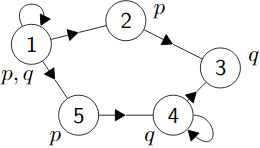
\includegraphics[width=70mm]{images/naturalnumbers.png}
  \end{center}
  \caption{Graphical representation of a basic Kripke model}
  \label{fig:kripkemodel}
\end{figure}
\subsection{Monotonicity}
We say that a function $f:\powerset(S) \rightarrow \powerset(S)$ is monotonic if for all sets $U, V \subseteq S$, if $U \subseteq V$ then $f(U) \subseteq f(V)$. This means that a monotonic function is entirely non-increasing or non-decreasing. Monotonic functions are required when defining fixed points.
\subsection{Fixed Points}
We have two fixed points of a finite set $S$ and a function $f$. The greatest fixed point or $GFP(f)$ is the fixed point which has the largest cardinality, the least fixed point or $LFP(f)$ is the one with the lowest cardinality.
\\\\
We say a point is fixed with regards to a monotonic function $f$ when:
$$f(f(S)) = f(S)$$
From this we can compute the GFP and LFP of a set S as follows:
$$LFP(f) = \bigcup_{n \in \mathbb{N}}f^n(\emptyset) \qquad GFP(f) = \bigcap_{n \in \mathbb{N}}f^n(S)$$
\subsection{Bisimulations}
If we take two Kripke models $(W, R, h)$ and $(W', R', h')$ and let $t\in W$ and $t'\in W'$. A bisimulation between them is a relation $B \subseteq W \times W'$ computed by the following algorithm:
\begin{enumerate}
\item $B(t, t')$
\end{enumerate}
For every $u \in W$ and $u' \in W'$ such that $B(u, u')$
\begin{enumerate}[resume]
\item All atoms that hold at $u$ hold at $u'$
\item If $v \in W$ and $R(u, v)$ then there is $v' \in W'$ with $R'(u', v')$ and $B(v, v')$
\item If $v' \in W'$ and $R(u', v')$ then there is $v \in W$ with $R(u, v)$ and $B(v, v')$
\end{enumerate}
\section{Page Comparison Techniques}
\subsection{Hamming distance}
The hamming distance is a simple measure of how different two strings of length $n$ are. It is defined as:
$$d(x, y) = \sum_i^nf(x_i, y_i)$$
where:
  \[
    f(m,n) = \left\{\begin{array}{lr}
        0 & \text{for } m = n\\
        1 & \text{for } m \neq n
        \end{array}\right\}
  \]
\subsection{TF-IDF}
TF-IDF is one of the industry standard open source methods of evaluating how important a word is to a document~\cite{tfidf}. It is built upon 2 measures:
\\\\
\textbf{TF: Term frequency} is computed using the ratio of the number of times the term appears with relation to the length of the overall document.
\\\\
\textbf{IDF: Inverse document frequency} measures how important a term is within a corpus of documents. It first needs to ignore words that appear commonly in written text such as `is', `of' and `that' and then compute the ratio of the total number of documents by the number of documents which contain the term.
\\\\
Cantina used this method by calculating the most important terms in the page and then assessing whether it appears in the top of Google's search results~\cite{cantina}. If it did not, then it was likely to be a copy of a legitimate page, and thus classified as potentially phishing.
\subsection{DOM Trees}
Often when comparing the similarity of two web pages, it is useful to look at DOM trees. Browsers compute DOM trees as an internal representation of the HTML structure of the page. There is an assumption that if two pages construct the same DOM tree then they will have identical layouts.
\begin{figure}[h]
  \begin{center}
    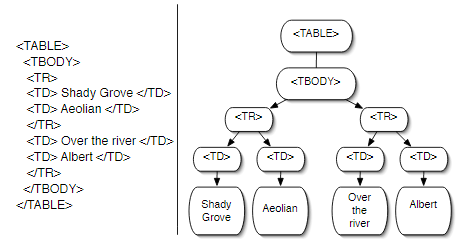
\includegraphics[]{images/domtree.png}
  \end{center}
  \caption{Example of a DOM tree representation~\cite{layoutsimilarity}}
  \label{fig:domtree}
\end{figure}
\\
Le Dang Nguyen et al. developed an algorithm to compute the similarity of two websites using the extracted DOM trees~\cite{domtreestructure}. They proposed the usage of a genetic algorithm which uses a fitness function when comparing the vertices of two graphs and checking if there is a corresponding vertex in the graph that we are comparing to.
\\\\
A contrasting method proposed by Qian Cui et al. was to take the DOM trees and compute the proportional distance using tag vectors~\cite{phishingovertime}. The tag vectors count how many of each tag appear in each DOM tree, and then compute the Hamming distance between the counts on each tree. This allows us to compare two similar pages that have been re-arranged by the attacker in order to make the pages seem different.
\\\\
Although comparing DOM trees is generally a fairly accurate way of computing the similarity between two pages, attackers can make a concious effort to avoid these methods and compute very different DOM trees with similar visual output.
\section{Image Comparison Techniques}
\subsection{Template Matching}
When a template image is to be detected within a larger source image we can use template matching to compare them.  The template image is compared to the source image by sliding it. At each point we compare how many pixels in the template image match with the target image and in each iteration we slide one pixel to the right \cite{templatematching}.
\\\\
Template matching is a naive approach which only accepts images that are exactly taken from the target image and that have not been scaled or changed. It is however a very fast approach and is useful in some scenarios. A simple similarity measure for template matching is cross-correlation which computes the sum of pairwise pixels in the image. This is a good metric for the similarity however it can be skewed by bright images that do not correspond with the target.
\subsection{Affine Transformations}
Affine transformations are linear translations that occur with 2D images~\cite{affinetransform}. Often when comparing images, affine transformations occur intentionally or unintentionally. There are 4 common affine transformations as can be seen in table \ref{table:affinetransformations}.
\begin{table}[h]
  \begin{center}
    \def\arraystretch{2}
    \begin{TAB}(r,1cm,2cm)[5pt]{|c|c|}{|c|c|c|c|}
      Translation & 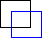
\includegraphics[]{images/translation.png} \\
      Scale & 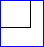
\includegraphics[]{images/scale.png} \\
      Shear & 
\includegraphics[]{images/shear.png} \\
      Rotation & 
\includegraphics[]{images/rotation.png} \\
    \end{TAB}
  \end{center}
  \caption{Table of all possible affine transformations and transformation matrices~\cite{affinetransform}.}
  \label{table:affinetransformations}
\end{table}
\subsection{FasT Matching}
FasT matching is a technique developed by Simon Korman et al. for approximate template matching under 2D affine transformations~\cite{fastmatching}. When using a standard architecture, this technique requires processing time of a few seconds. An example is shown in figure~\ref{fig:fastmatching}.
\subsection{Cascade Classification}
Cascade classification is a techinique used primarily in computer vision in order to detect objects or faces within video streams. These classifiers typically use a model which is trained with a series of negative images which do not contain the object, as well as a series of positive images of the object in various positions within different frames.
\\\\
The term `cascade' is used since the resultant classifier is composed of several simpler stages which are applied to a region of interest, and accepted if a certain threshold of these stages succeed~\cite{cascadeclassification}.
\subsection{Haar Classifier}
The Haar feature-based cascade classifier developed by Viola and Jones in 2001 is a rapid detection algorithm with a high degree of accuracy; however the training of the model is a slow process \cite{haarclassification}. Motivated by the problem of face detection within live video, the algorithm can process roughly 15 frames per second.
\\\\
The classifier works by detecting features within a very large feature space of the image, the feature space is much larger than the number of pixels in the image itself. To reduce the feature space, each weak classifier in the cascade of classifiers is based on a single feature, and on each iteration a set of classifiers is chosen, therefore reducing the feature set. During detection, the small set of features from the training process is loaded and attempted to be detected within the image.
\subsection{Local Binary Patterns Classifier}
LBP classifiers are the more recent approach for object detection within images, it works by thresholding the $3 \times 3$ neighbourhood of each pixel and considering the result as a binary number for the pixel \cite{lbpclassification}. Inside the image, each detected feature can be considered as a cascade of patterns within the pixel radius, which is then added to the trained model.
\begin{figure}[h]
  \begin{center}
    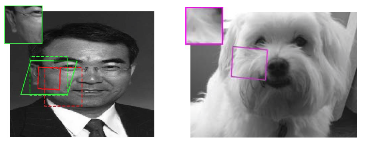
\includegraphics[]{images/fastmatching.png}
  \end{center}
  \caption{Example of FasT matching algorithm results~\cite{fastmatching}}
  \label{fig:fastmatching}
\end{figure}
\subsection{OpenCV}
OpenCV is an open source computer vision library in Python and C++. It was designed for computational efficiency with all of the computationally expensive code written in C++ and interfaces in both Python and C++ through the use of Cython \cite{cython}\cite{opencv}. 
\section{Web Capture}
In order to process pages and output a classification, we need a method of collecting the pages' information for analysis.
\subsection{WARC}
The web archive file format (WARC) is a complete packet capture of a page which aggregates multiple digital resources into a single archive \cite{warc}. It is a complete capture of the information a browser retrieves when it visits a specific page. This includes the HTML, status codes and pages which the browser has been redirected to.
\subsection{Common Crawl}
WARC files are the preferred form of storage for Common Crawl. Common Crawl is an open source web crawl with large amounts of crawl data available open source for anyone to analyse. The aim of the project is to make the web open to all rather than large organisations like Google with their resources. There are petabytes of web crawl data spanning over four years in which they have been operating.
\section{Client Server Architecture}
In Python there are two main ways in which we are able to create a client server architecture for communication with the program.
\subsection{TCP}
TCP communication is built into Python using the \texttt{socket} library. It is very simple to simply open a port for communication on the local networking protocol. Data can be sent byte encoded over the channel in a very fast manner. However there are issues with ease of use and coupling since a client needs to be built with its own interface and then needs to connect to the server in order to transmit data back and forth.
\subsection{Flask}
Flask is a module within Python which allows us to quickly create a server on \texttt{localhost} where we can implement a Rest API for communication. With Flask we do not need to create a dedicated client, we can simply query the browser and read the results with JSON.

\chapter{Implementation}
\section{Candidate URL Collection}
As with most machine learning problems, the first issue we encountered was how to collect large amounts of data to train and test the classifier. Lastline as a company deal with WARC files and PNG screenshots, so the classifier was required to be able to process these files.
\\\\
For the malicious data collection we fetched URLs hourly over the course of 2 weeks from the OpenPhish feed and the IllegalFawn feed~\cite{openphish}\cite{illegalfawn}. These two feeds are provided by independent security researchers who do not publicly disclose their methodologies for obtaining these live phishing URLs, however make the lists public in order to update browser blacklists.
\\\\
Once these URLs are collected hourly, some pre-processing is done to avoid overloading the analysis infrastructure:
\begin{itemize}
    \item URLs which have already been analysed are immediately discarded
    \item Up to two URLs for each public suffix are retained, these public suffixes are obtained from the Python \texttt{publicsuffix} library \cite{publicsuffix}
    \item A maximum limit of 1024 URLs are retained per hour
\end{itemize}
For collection of benign data we needed a method of filtering out all malicious data from a large crawl of data. We used Common Crawl for the bulk of the data, however to actually filter out all malicious data from an arbitrary crawl data set would require the classifier which we are trying to create. We assumed that generally popular websites which were in the Alexa list would be very unlikely to be benign so we obtained the Alexa top 1 million list, randomly selected URLs from this list and then we filtered the Common Crawl data with URLs where the top level domain name was in our set of selected URLs \cite{commoncrawl}\cite{alexa}.
\\\\
We collected the WARC files for both the benign and malicious URLs in the same way in order to have consistency in the input data for our classifier. To do this, we submitted the URLs to the Lastline sandbox where the URL is visited using Internet Explorer 8 on a Windows 7 machine. The sandbox then monitors the activity performed by the browser and saves the capture of the network traffic generated in a PCAP file which is then converted into a WARC file.
\section{WARC Parsing}
In order to process the data we needed to extract the components from the WARC files into a Numpy array so that they could be fed into the classifier. In order to process each WARC file, we used the Warcio library which provided an iterable array of each record in the file \cite{warcio}.
\\\\
\textbf{URL}\\
During the WARC collection process, Lastline's sandbox kept a track of the target URL for each WARC capture and saved it into a CSV file. When processing each file, we obtained the corresponding URL from the CSV file generated by the sandbox.
\\\\
\textbf{HTML}\\
Due to the random ordering of the WARC file, it was not possible to simply obtain the HTML content of the first record in the file. We had to find the first HTTP response where the \texttt{WARC-Target-URI} corresponds to the URL found in the CSV file. If however, this record happened to be a 301 or 302 redirect, we would then find the corresponding record which it redirected to and extract the HTML from there. 
\\\\
\textbf{Text}\\
In order to extract the text, we needed to use BeautifulSoup to parse the HTML \cite{beautifulsoup}. We obtained all content which was not contained in \texttt{style}, \texttt{script}, \texttt{head} or \texttt{title} tags.
\\\\
\textbf{Screenshot}\\
The screenshot was obtained in the candidate URL collection by using Firefox's screenshot terminal interface with the \texttt{--screenshot} option. The path to the corresponding screenshot was stored in the array to avoid over usage of memory so that it could be read when needed.
\\\\
\textbf{Status}\\
In order to process the status, we obtained the HTTP status from the first record that the URL pointed to. Although we were not necessarily processing the HTML and resources from the initial record relating to the URL, we believed that the status of the first record was the most informative. With a 301 redirect for example, the final record would have a status code of 200 so we would lose information about the initial status if we only considered the status of the final record visited.\\\\
\textbf{Resources}\\
For the resources, we decided to extract the images which were contained within the WARC files as images which the pages would fetch when they were rendering the page. For this we needed to find all records in the archive and extract the bytes of pages which had the HTML content type as \texttt{image/png}.
\section{Pipeline using Cantina and DOM Comparison}
We planned to implement a hybrid classifier which combined a variety of different approaches as features in a machine learning algorithm. We decided for an initial implementation to use elements of the Cantina classifier in addition to computing bi-simulations between the DOM trees of new pages to classify and existing known phishing pages \cite{cantina}.
\\\\
As explained in section \ref{motivation}, Cantina's implementation of phishing detection involved obtaining the textual content of the page, performing the TF-IDF algorithm to find the words with the highest importance, and then assessing if the page appeared in the top n results of a Google search for these keywords.
\subsection{Pipeline}
We needed to initially create the pipeline to process the data and help us to train our classifier using the feature extractors that we were going to create. We created a basic initial pipeline which used a Logistic Regression module to serve as our classifier.
\subsection{TF-IDF}
In order to compute the inverse document frequency of the words in the page we needed a word corpus to compare against. We used the British National Corpus provided by Oxford university which is a 100 million word collection~\cite{bnc}. The words contained in the corpus contain other languages but mainly consist of British English words.
\\\\
The usage of the British National Corpus brought in biases to the classifier. Pages which did not originate in Britain would use terminology that may not appear as frequently in the corpus and would therefore cause words in certain web pages which are common in other languages to have a high TF-IDF score. Considering also that the word corpus is static, and has been collected over a certain period of time, meant that the corpus would not classify words which may become more commonly used or be created in the future as well. 
\clearpage
\subsection{Google}
In order to search Google programmatically, there were three options: \\\\
\textbf{API Usage}\\
Custom Search is a REST API provided by Google to allow website owners to implement search functionality within their own websites. The API would crawl the website which the owner used and then provide a search functionality within that website. Inside the API configuration, there is also an option to include results from the web. We used this to generate an API key which searched the entire web and disabled the site search functionality within the API.
\\\\
This method was quite fast and reliable due to the Python's interface which Google provided, however there are limitations:
\begin{itemize}
    \item Google has deprecated the API in the past and it is not currently being maintained with a risk of being deprecated or deleted at any point since Google do not guarantee its uptime.
    \item Usage limits mean that there are only 100 free queries to the API per day up to a limit of 10,000 queries per day at a cost of \$50 per day.
    \item Google do not provide the same results ordering on their website as they do with the API queries.
\end{itemize}
~\\
\textbf{Manual Web Scraping}\\
We used the \texttt{urllib} package within the Python core modules to query Google and return the HTML result and then used BeautifulSoup to parse the output \cite{beautifulsoup}. This also provided other limitations:
\begin{itemize}
    \item Google implement abuse and automation blocking techniques such as CAPTCHA and IP address barring \cite{captcha}.
    \item The method is much slower than the API calls due to the HTML parsing overhead.
    \item The method would have to be updated if Google were to modify their HTML page structure.
\end{itemize}
~\\
\textbf{Querying Other Search Engines}\\
There were two other main search engines which we attempted to use instead of Google. Bing was the next option which had an API priced at \$7 per 1000 queries with no limit; however this was still far too expensive \cite{bing}. DuckDuckGo was also another option who were willing to provide an API for free, however they are an aggregator service for different search engines and as such are unable to provide this service publicly without violating the terms and conditions of the services which they obtain their data from \cite{duckduckgo}.
\\\\
Faroo is a service who attempted to provide searching as a free service, however their crawling resources are too small and most of their search results are extremely old and therefore would not be useful for our classifier \cite{faroo}.
\subsection{DOM Comparison}
For the DOM comparison, we obtained three examples of malicious and three examples of benign pages and used PyPi's \texttt{html-similarity} module to compute the \texttt{structural\_similarity} and \texttt{style\_similarity} of the pages \cite{pypi}.
\\\\
Since we made the assumption about the pages using derivatives of different phishing kits, the \texttt{structural\_similarity} of the HTML we assumed to be quite similar with phishing pages but not necessarily the \texttt{style\_similarity}.
\\\\
Although this seemed to be a good metric some of the time, there tended to be a lot of noise in the results with pages which are stylistically very different but still obtained a high \texttt{style\_similarity} score. In addition, we were unable to compare against a large number of pages due to the added time complexity of the module.
\section{Current Pipeline}
There were many issues with the previous pipeline which caused issues with scalability. Not being able to query Google as frequently as we wanted was a problem since we needed to train and test our model on around 40,000 examples and we wanted to run long evaluation scripts to test different parameters within our classifier. In addition, the classifier is intended to be used as part of a live classification system which would constantly be run on new data, in this scenario, the API limits provided would be insignificant.
\\\\
DOM comparison and TF-IDF algorithms caused temporal issues. Our classifier would not be able to classify new examples in the future when the language used had evolved, as well as when the evolution of phishing kits had significantly changed the HTML structure of new attacks. We tried to approach the new classifier such that, as much of the temporal information as possible was able to be obtained from the training data when updating the model, so that the model was able to classify new examples if it was trained regularly.
\\\\
For each element in our pipeline we have given a robustness score. We have attributed this score to how hard we think it is for attackers to change their pages in order to not be detected.
\begin{figure}[h]
  \begin{center}
    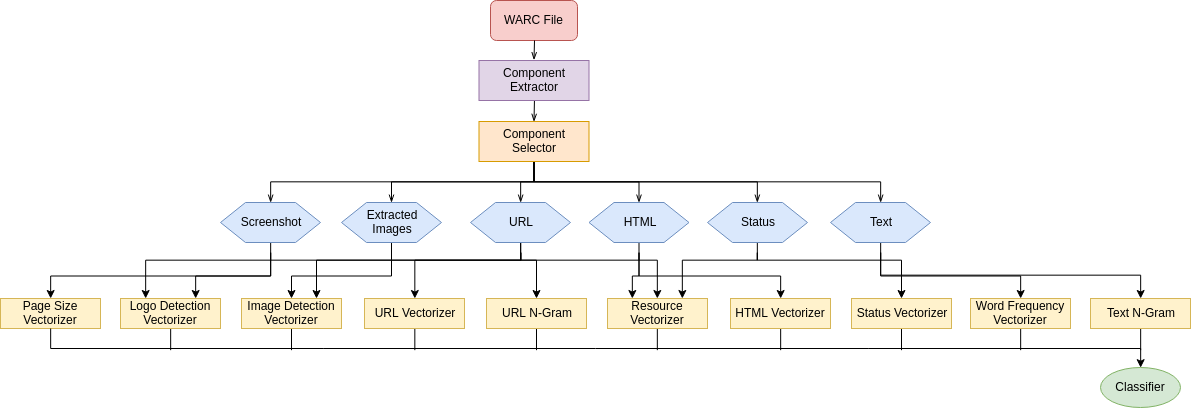
\includegraphics[width=155mm]{images/pipeline.png}
  \end{center}
  \caption{Data flow diagram of current pipeline}
  \label{fig:currentpipeline}
\end{figure}
\subsection{Item Selectors}
We structured the pipeline as a set of feature extractors and a feature union of each of the modules that we wanted to implement. This can be seen in figure \ref{fig:currentpipeline}.
\\\\
With this we implemented a set of item selectors which returned the components which the module needs to run. This is from the set of components extracted during the WARC parsing process.
\subsection{N-Grams}
We implemented n-grams within our classifier in order to detect common patterns on phishing pages. There are common words which occur within the text of a phishing page such as 'password' and 'alert'. N-grams allow the classifier to automatically gain insights of common string combinations.
\\\\
We have also applied n-grams to the URL in order to detect common words such as 'bank' or 'login'. We varied the value of n in our n-grams in order to find a balance between number of features and information gain.
\\\\
We have given the n-gram modules a high robustness score since attackers need to use terminology in both the URL and the page textual content in order to lure the user into entering details.
\clearpage
\newgeometry{margin=0.7in}
\subsection{URL Vectorizer}\label{urlvectorizer}
\begin{center}
\begin{longtable}{ |>{\raggedright\arraybackslash}p{0.19\textwidth}|>{\raggedright\arraybackslash}p{0.13\textwidth}|>{\raggedright\arraybackslash}p{0.29\textwidth}|>{\raggedright\arraybackslash}p{0.29\textwidth}| } 
\hline
\textbf{Name of feature} & \textbf{Robustness\footnotemark} & \textbf{Feature Description} & \textbf{Robustness Discussion} \\
\hline
\endhead
\footnotetext{We define robustness as how easy it would be for an attacker to circumvent the particular feature}
URL contains `@' symbol & Low & `@' symbols are common in phishing URLs, they usually occur when the URLs include an email address as one of the GET variables. & To avoid this, the attacker can submit variables by POST methods instead. \\
\hline
Hostname contains `-' symbol & Low & Many malicious URLs use wordpress websites without modification, leaving elements in the URL such as `wp-admin'. They may also use `-' in their URL if they wish to join to a legitimate hostname, for example `www.security-hsbc.co.uk'. & The main usage of hyphens is wordpress usage without modification of the path names, to change this the attacker needs to simply modify the path name in the wordpress settings. \\
\hline
URL contains brackets & Low & Brackets appear in URLs where malicious pages upload files which they have previously multiple downloaded, for example doc(1).pdf. & This happens very rarely but it is often a sign of an attacker who has invested a small amount of effort into the page. If the attacker wished to circumvent this, they need to simply rename the files. \\
\hline
Number of Subdomains & Medium & Used as a common method to put a legitimate URL as a subdomain of a problem URL such as \url{http://bank.barclays.com.bit.ly}. & This can be avoided but is a common technique so it is unlikely for the attacker to do so. \\
\hline
Subdomain contains TLD & Medium & Comparing the subdomain of the URL against the TLD list obtained from the Mozilla public suffix list which is a well maintained up to date list of TLD suffixes \cite{publicsuffixmozilla}. & As we can see in section \ref{urlobfuscation}, this is a common technique used by attackers and as such is a robust feature to detect. \\
\hline
Path contains TLD & Medium & Comparing the path of the URL against the TLD list obtained from Mozilla public suffix list \cite{publicsuffixmozilla}. & If the attacker was unable to create a subdomain on the host, this would be the next most favourable option to try and trick the victim. \\
\hline
Path contains `=' symbol & Medium/Low & GET requests are common within phishing attacks because they are easier to process than POST or PUT requests. & There is no way to avoid using `=' symbols if GET requests are being used and since they are common, it is a robust feature to detect. \\
\hline
Hostname contains number & Medium/Low & Commonly occurring when hashed information is stored in the URL. & Often used as a technique for attackers to hide sensitive information in a GET request. \\
\hline
URL contains cyrillic characters & Medium/Low & Cyrillic characters can look very similar to English characters, there have been phishing attacks in the past where attackers used these characters to register domains where the URL looks exactly the same as the official page \cite{xudongs}. & Although many major browsers have taken preventative measures to tackle this issue, this feature is often a strong signal that the attacker may be using such methods.\\
\hline
Shortened URL & Medium/Low & Although users have legitimate reasons to use URL shortening services, it is also a common technique to mask the malicious URL from the victim. \newline\newline Using a frozen list of URL shortening services is the only way to detect the usage since there is no way our classifier can learn which new services are to be created in the future. & Since we are forced to use a frozen list, the attacker is able to find a URL shortening service that we have not already detected if they wish to circumvent this feature. \\
\hline
Target in subdomain & Medium/Low & Check if a frozen set of targets exists in the subdomain of the URL. Targets are in a frozen list but get updated using the PhishTank API \cite{phishtank}.  & We use n-grams for learning new words that are being used as a more robust feature. However checking for a target in a list of words is a useful feature with less robustness but also has a very low performance cost.\\
\hline
Trigger in path & Medium/Low & Check if a frozen set of trigger words exist in the path of the URL. & If the list is obtained, these triggers can be easily avoided however the trigger words are often words that attackers need to use in order to fool their victims. \\
\hline
Target in path & Low & Check if a frozen set of targets is in the path. & It is not common for the targets to be in the path and it is easily avoided by the attacker, however the feature is very strong when detected. \\
\hline
Changed port & Medium & Check if the port has changed, it is common for attackers to compromise the DNS records of legitimate websites and redirect traffic on an unused port to the malicious page. & If the attacker is able to modify the DNS, they will often use a different port on the website they gained access to so this is a robust feature. \\
\hline
Misspelled target in URL & Medium & This can often be useful as a separate feature than simply detecting the target in the URL. & Misspelled targets is one of the most common ways in which attackers attempt to fool users that they are on the legitimate page. Therefore, in addition to detecting the correctly spelled URL, the misspelling is also important to detect. \\
\hline
Length & Medium & Number of characters in the URL.  & In addition to the other features, malicious URLs are generally longer than benign URLs, since they attempt to hide extra information using methods described above.\\
\hline
Uses HTTPS & Medium & Although it is now more common for phishing pages to employ HTTPS according to the latest report by APWG, in order to seem legitimate, for most websites it is not worth the effort for the attacker to install an SSL certificate \cite{apwg}. & To circumvent this feature, attackers can use SSL more in the future, however with the short time to live of most phishing pages and that SSL certificates are already freely available today with letsencrypt, attackers are unlikely to start using HTTPS more in the future \cite{letsencrypt}. \\
\hline
Size of query & Low & This is the size of the query in the page, for example in \url{https://www.google.com/q=test} the query length would be the length of the word `test' which is four.  & Queries can easily be avoided by attackers however it still seems to be a strong feature for phishing URLs. \\
\hline
\end{longtable}
\end{center}
\restoregeometry
\subsection{Word Frequency Vectorizer}\label{wordfrequencyvectorizer}
Using the TF-IDF algorithm on the textual content of the page was a useful heuristic in the previous version of the pipeline, however we were reliant on the usage of the static word corpus. To solve this we decided to use the combination of the text from all of the pages within the training set as our word corpus. Therefore, when we trained our model on new examples, the word corpus would be updated. In addition the corpus would be relevant to the pages which we are classifying upon, meaning that the language bias introduced by using the British National Corpus would be removed.
\\\\
We believe the robustness of this vectorizer to be much higher than the previous implementation since the words that are important to a page are not from a single source. For this reason, if the attacker wanted to circumvent this feature, they would have to find words that are uncommon in web pages today rather than querying the British National Corpus and using words which have a low ranking.
\subsection{Status Vectorizer}
We wanted to investigate the HTTP status of the page and use this as a feature for the classifier. We initially considered using an n-gram for the status however this caused a large number of features to be created which was not useful for our classifier. Therefore we decided to extract the base status number from the HTTP status line and create features for common status numbers we deemed to be relevant.
\\\\
The robustness of the status vectorizer is very high because there is no way for the attacker to manually spoof the HTTP status response code that we obtain. We are able to detect re-directions which are very common in phishing pages and combined with the HTML, we can further detect if a page is attempting to fake an HTTP status and returning a different page. For example we can detect if the page is in fact found with a status code of 200 but the website is attempting to serve a fake 404 page instead.
\newgeometry{margin=0.7in}
\subsection{HTML Vectorizer}\label{htmlvectorizer}
\begin{center}
\begin{longtable}{ |>{\raggedright\arraybackslash}p{0.19\textwidth}|>{\raggedright\arraybackslash}p{0.13\textwidth}|>{\raggedright\arraybackslash}p{0.29\textwidth}|>{\raggedright\arraybackslash}p{0.29\textwidth}| } 
\hline
\textbf{Name of feature} & \textbf{Robustness} & \textbf{Feature Description} & \textbf{Robustness Discussion} \\
\hline
\endhead
Page uses a favicon & Very Low & Basic feature which checks if the page has a favicon present or not.  & Although attackers typically do not use favicons, it is simple for the attacker to add one and thus circumvent this feature.\\
\hline
Number of forms & Low & We used this feature rather than the boolean value of whether forms are present on the page because we believe that phishing pages generally only use a single form element and other benign pages may use multiple forms. & The attacker can create invisible forms in order to increase the number of forms on the page.  \\
\hline
Number of password fields & Low & Malicious pages tend to contain a single form with a single password field. & In the same manner as number of forms, the attacker can add invisible password elements as well.\\
\hline
Number of iframes & Medium/Low & Iframes are HTML components which are generally not used frequently anymore but still remain prevalent in old phishing kits. & This feature is trying to detect pages using older phishing kits directly without modification. However, if the phishing kit is reliant on iframes, for the attacker to change this would involve them having to rewrite that part of the kit to work without iframes which is time consuming.\\
\hline
Scripts to HTML ratio & Medium/Low& We assume that phishing pages generally have a low HTML page content, since they require only to convince and capture the user's data. However, many kits also use scripts heavily to capture as much information as possible. These pages will have a high script to HTML ratio. & If the attacker wishes to reduce their ratio, and they are using a lot of scripts, they would need to add copious amounts of invisible HTML code which could then become a feature itself to detect. It is also unlikely that the attacker would try and prevent being detected with such a feature. \\
\hline
Number of tags & Medium/Low & This feature indicates the size of the page ignoring the amount of text inside the tags. & In order to change this the attacker would also have to create a lot of invisible tags, as in for the scripts to HTML ratio feature.\\
\hline
Size of page & Medium/Low & This gives us the number of characters in the HTML page. This feature in conjunction with the number of tags allowed us to detect pages which have a large amount of text inside tags such as paragraph tags. & In order to change this the attacker would have to add text or padding into the page to increase the length which they are unlikely to do if they wish to seem legitimate as a page.  \\
\hline
\end{longtable}
\end{center}
\restoregeometry
\subsection{Resource Vectorizer}\label{resourcevectorizer}
The resources on the page, such as the form actions, and the links of the page, are good items to investigate. We believe this since phishing pages generally will have pages which are hosted on a different server, with links to the legitimate page, as well as potentially links to their page. They will also need to direct the form POST action, to a page which they are controlling, in order to store the phished credentials. For this analysis we investigated the URL, HTML and the status. The URL was important to know whether the links and form actions pointed to the same host, or alternative hosts, and inspecting the status also allowed us to detect, with the resources, whether the page was performing an HTTPS upgrade, or a redirect.
\\\\
We examined all the forms and links on the page and returned whether the form actions were empty, relative paths to the current page, pointed to a page on the current domain or pointed to external domains. We also went on to check whether the form actions pointed to a single host, or pointed to multiple different hostnames, since we believe that phishing pages generally want to direct all traffic to websites which they control. Once the user has logged in and they have phished the credentials, they would also usually redirect the user to the target page so as to not arouse suspicion.
\subsection{Screenshot Vectorizer}\label{screenshotvectorizer}
Whenever phishing sites wish to imitate a page, they need to try and convince the victim that they are on the page of the target. In order to do this, they would need to display the logo or some distinguishing visual signal of the target on the page. We hypothesised that if we were able to detect the target logo on the page, we would then be able to verify that the hostname of the URL matched with the hostname of the logo.
\\\\
We initially needed to collect a list of common targets so that we could select the top targets to detect. To do this we took the top 20 targets from PhishTank by querying their data sets and obtaining the targets which appeared with the highest frequency \cite{phishtank}.
\\\\
Once we had the top targets, we downloaded the first 10 images from Google image search results for these target names. We had to manually edit each image after this, in order to obtain a high-quality image, with the logo on a transparent background, and removing all textual content from the logo images. 
\\\\
We attempted a series of different image detection methodologies to try and detect the logo in the page. The fastest approach we found to be template matching, however, this did not work with affine transformations, and the logos on the page were usually different sizes and resolutions to the reference logos we had obtained.
\\\\
Our next step was to attempt to use feature matching in the hopes that logos which appeared on the page would detect a larger number of features than others. The results can be seen in figure \ref{fig:featurematchingcomparison}. As we can see in this figure, when trying to compare three different logos with an AT\&T phishing page, the PayPal logo matched the most key-points within the image, and the Microsoft logo matched very few key-points. We also noticed that the Microsoft logo only had four potential key-point matches, and as such for every page which we attempted to match it against, the number of matches returned was significantly lower than any other logo. There were also many matches with the logo and alternate points on the screenshot, usually the text, which did not correspond to the logo on the page. We could have attempted to correct for this using key-point clustering, however, the volume of direct matches between the target logo and the logo on the page, did not prove consistent enough to warrant this approach as being worthwhile.
\\\\
The next attempt was to use FasT matching, however there was no readily available implementation on the internet that worked well with Python \cite{fastmatching}. We also attempted to use feature matching with FLANN which keeps feature points matched which have a lot of nearest neighbours \cite{flann}. We thought that this could filter out our feature matching points so that we could keep only the points which corresponded to closely
\newgeometry{margin=0.7in}
\begin{figure}[!h]
\begin{center}
    \minipage{0.55\textwidth}
      \fbox{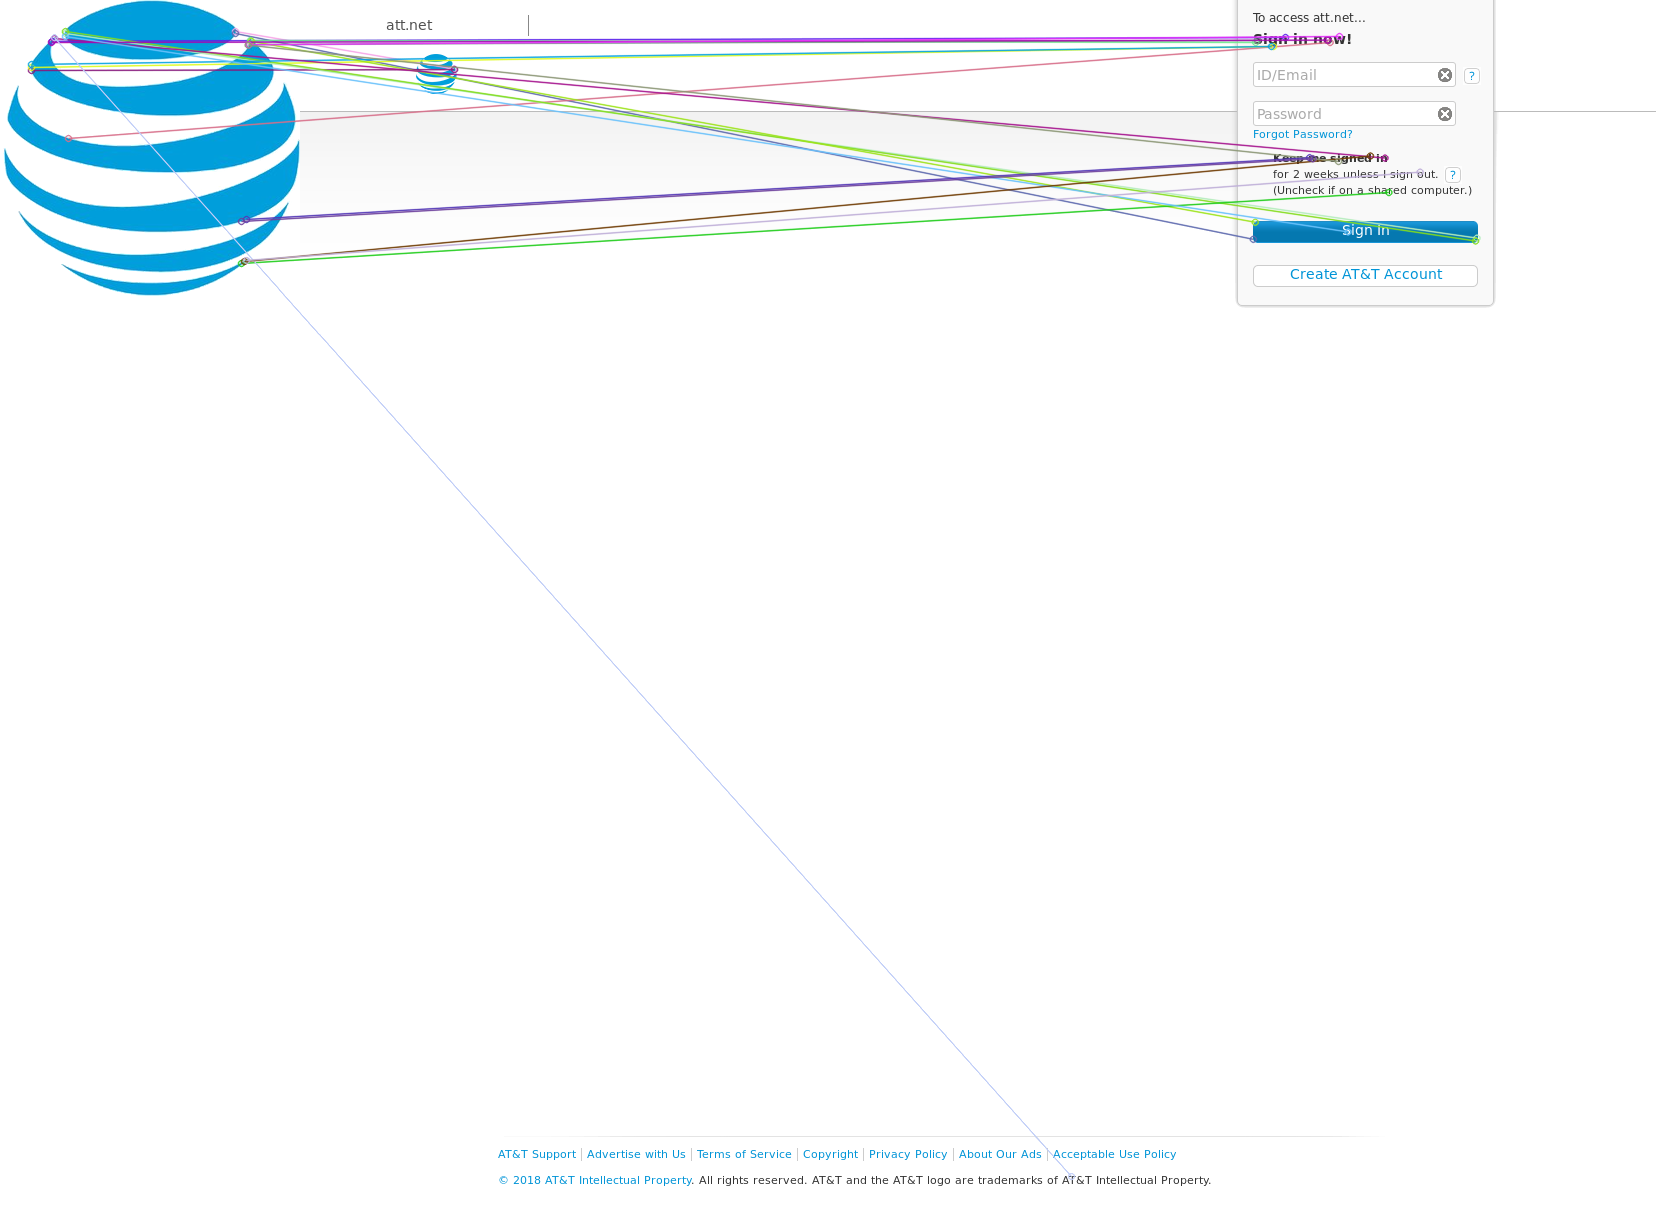
\includegraphics[width=\linewidth]{images/featurematchingat&t.png}}
      \\\\
      \fbox{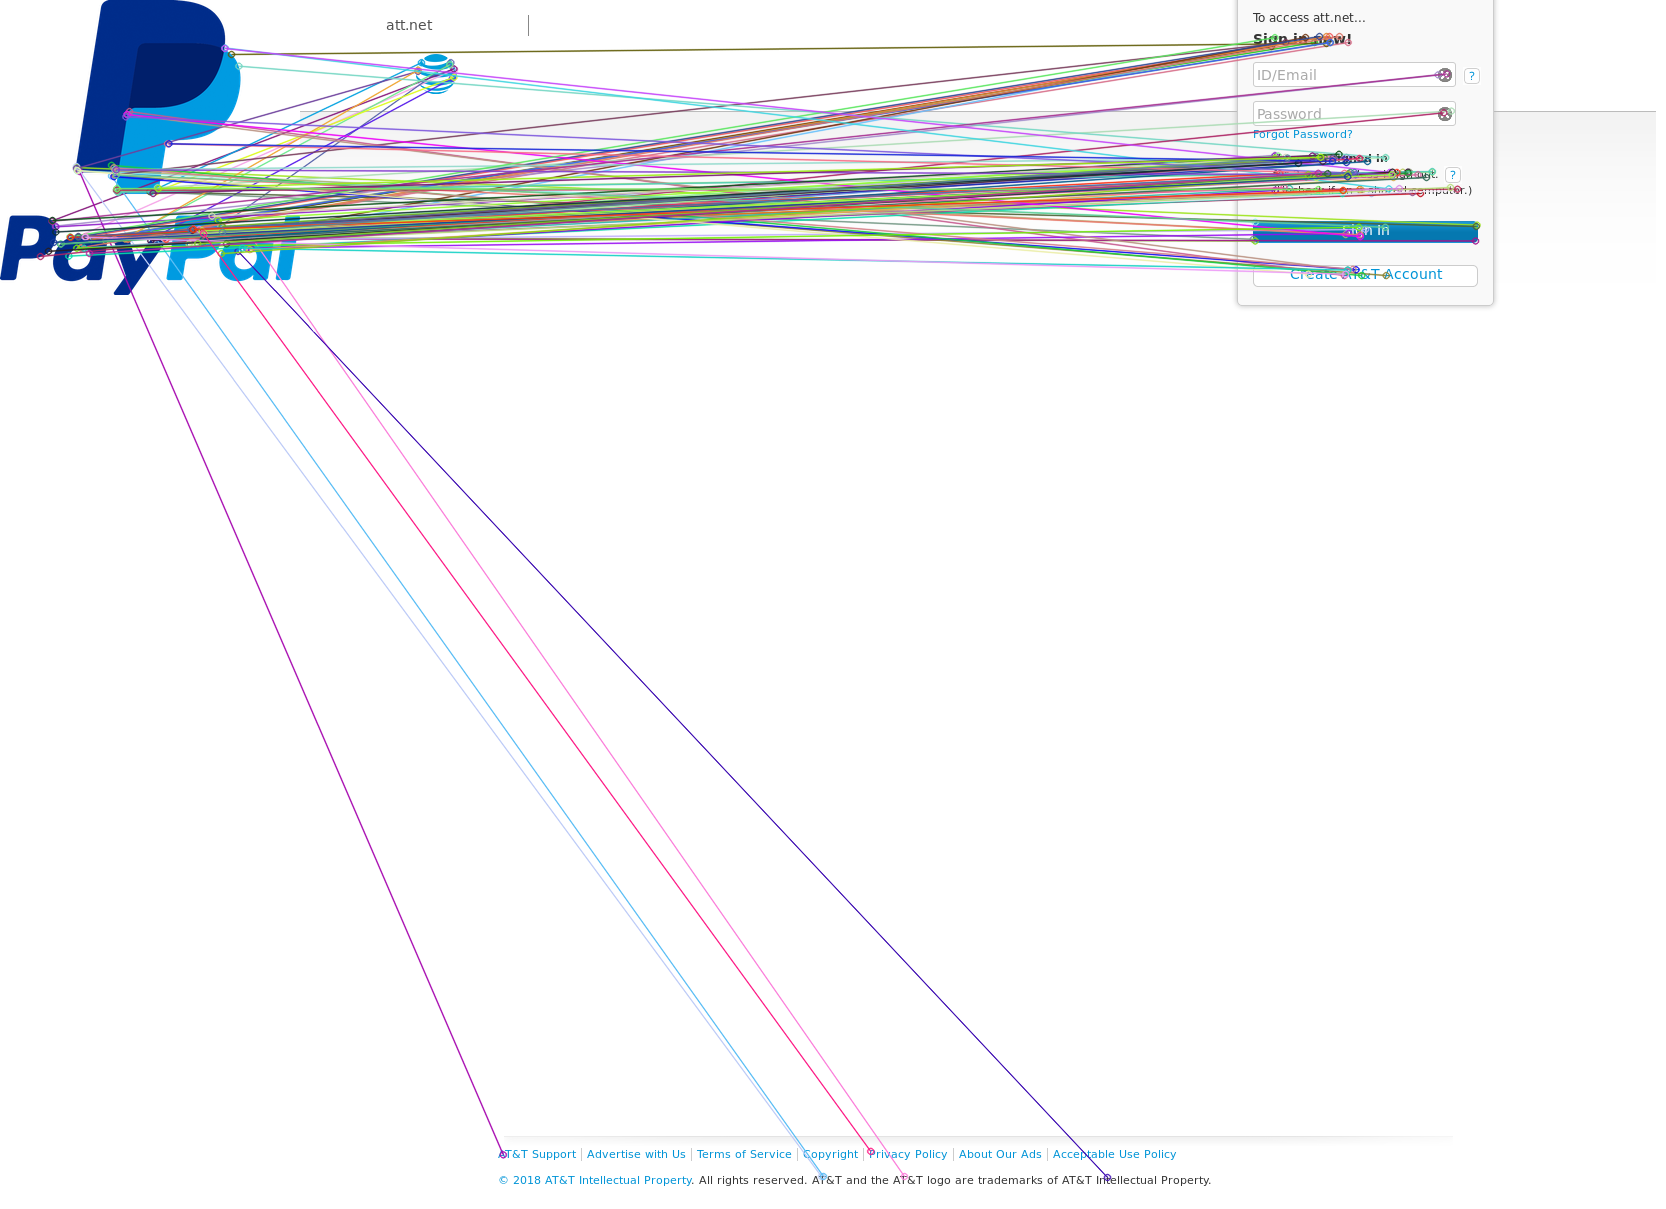
\includegraphics[width=\linewidth]{images/featurematchingpaypal.png}}
      \\\\
      \fbox{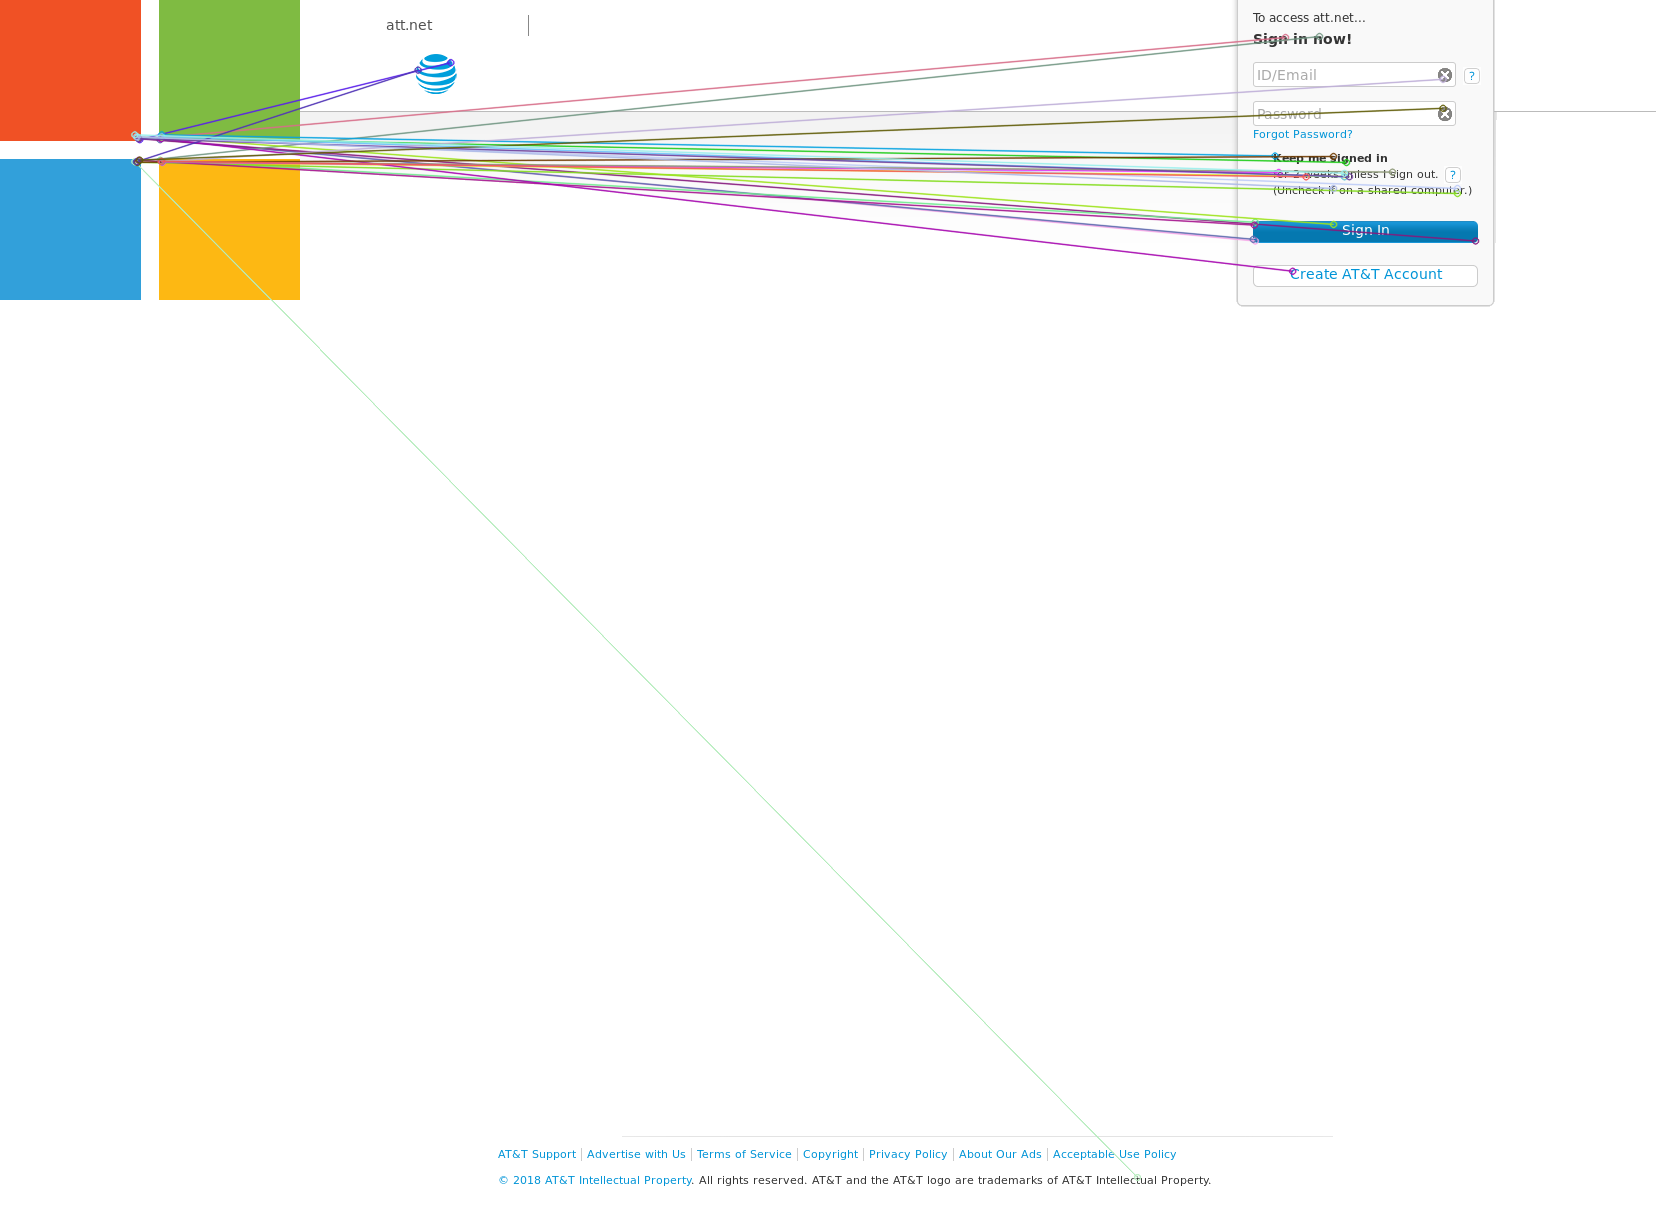
\includegraphics[width=\linewidth]{images/featurematchingmicrosoft.png}}
    \endminipage
\end{center}
\caption{Comparison of feature matching with AT\&T, PayPal and Microsoft logos on AT\&T phishing page}\label{fig:featurematchingcomparison}
\end{figure}
\restoregeometry
\noindent
grouped ones, as the logo on the page. This also did not work, because the feature detections within our screenshots were not strong enough that all the matches were filtered out as can be seen in figure \ref{fig:flannmatchingcomparison}.
\\\\
We then tried to use a cascade classifier, we trained the cascade classifier with the logos we obtained. To do this the classifier needs to learn with positive and negative images. For the negative images we obtained a set of random images from the internet, these images could contain any other graphics, however, they could not contain any logos from the ones which we wanted to train. We used OpenCV to generate a set of positive images with the logo, applying a set of transformations and then superimposing it onto the negative images using \texttt{opencv\_createsamples} \cite{opencv}.
\\\\
The training of each cascade classifier with the set of logos took approximately five hours to train per logo. The cascade classifier however worked relatively well for most logo detection as can be seen in figure \ref{fig:cascadematchingcomparison}.
\\\\
We did have issues with a large number of trained logos however. The Netflix logo worked extremely badly as can be seen in figure \ref{fig:cascadematchingnetflix}. We believe this may be due to the structure of the logo and that it does not have as many defining features. In the future careful logo selection and testing must be done before adding a trained cascade to the pipeline.
\\\\
We also noticed that many of the screenshots were very long and would incur a performance hit if we applied the cascade classifier to the entire image. For this reason, we cropped the height of the screenshots to be at maximum equal to their width. We did this so that we would reduce the time taken for the cascade classifier to try and find the logo as we made the assumption that the main logo of any page would be situated at the top of the page.
\newgeometry{margin = 0.7in}
\begin{figure}
\begin{center}
    \minipage{0.55\textwidth}
      \fbox{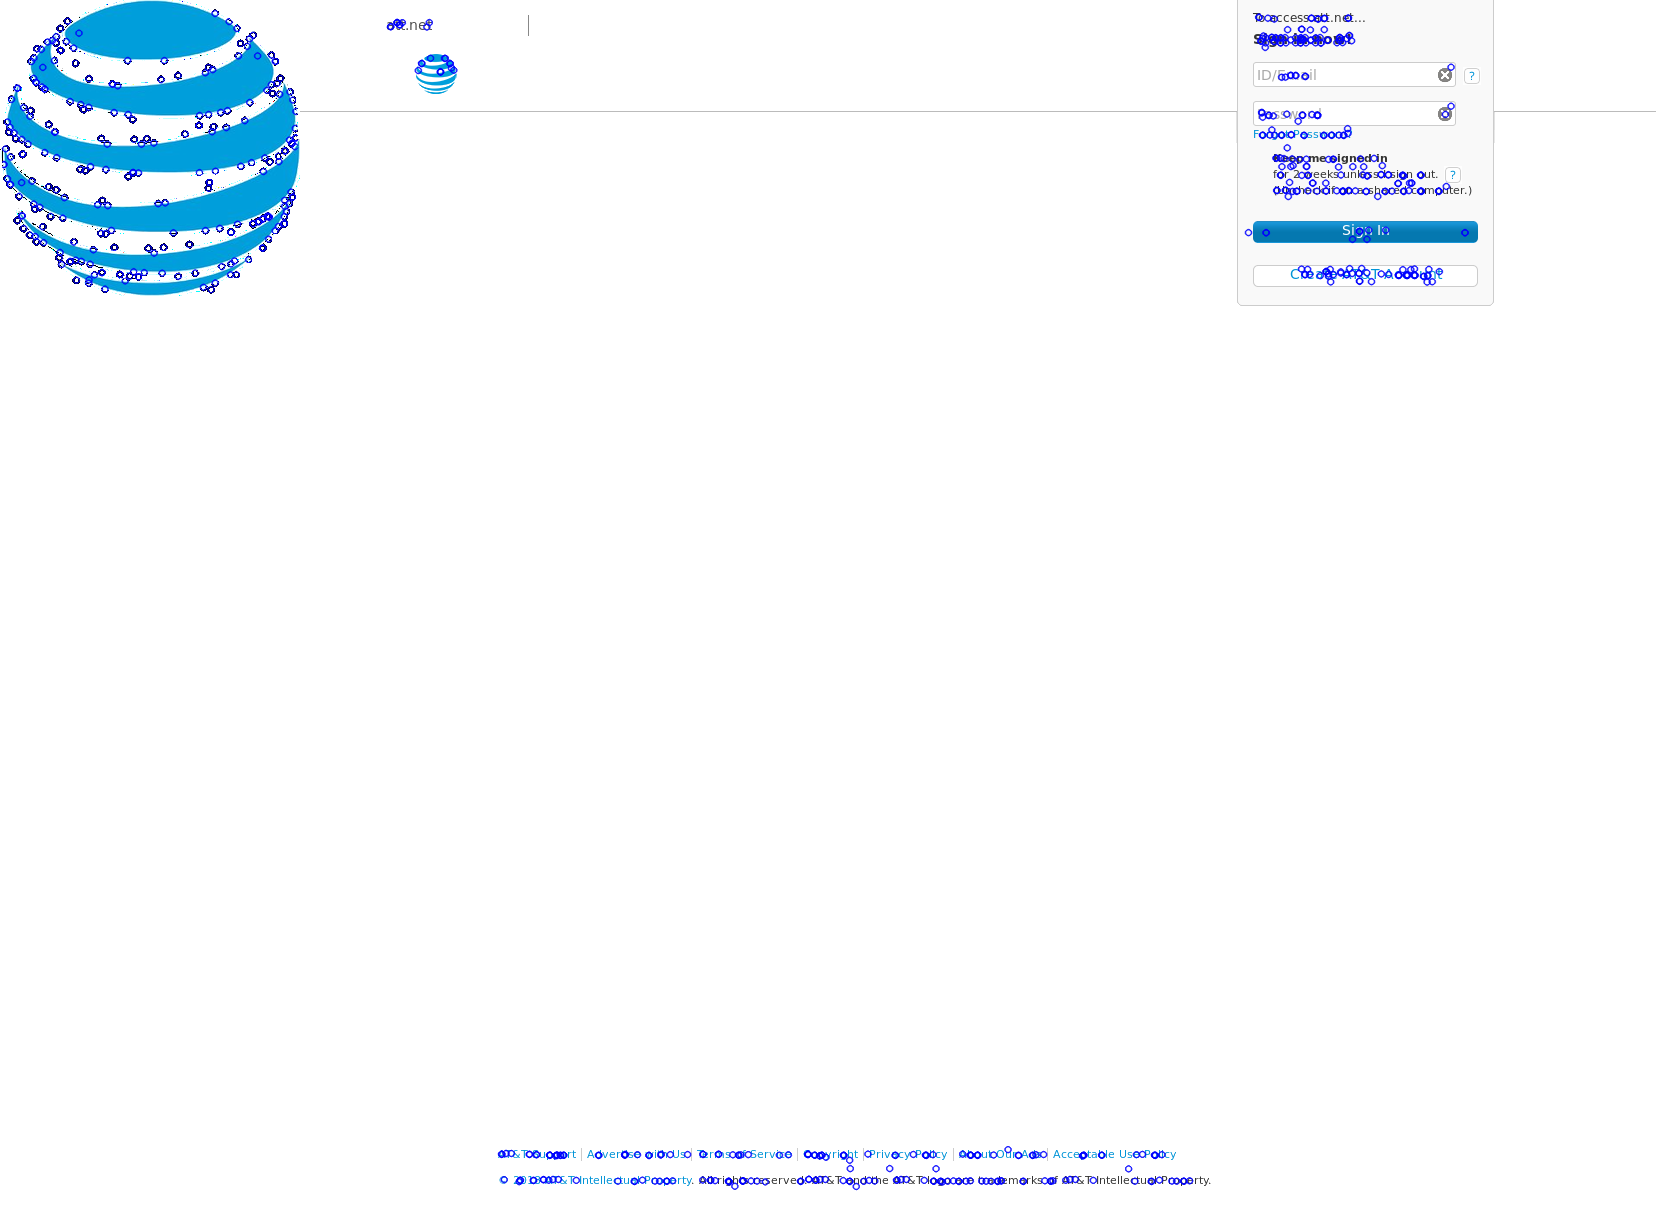
\includegraphics[width=\linewidth]{images/flannmatchingat&t.png}}
      \\\\
      \fbox{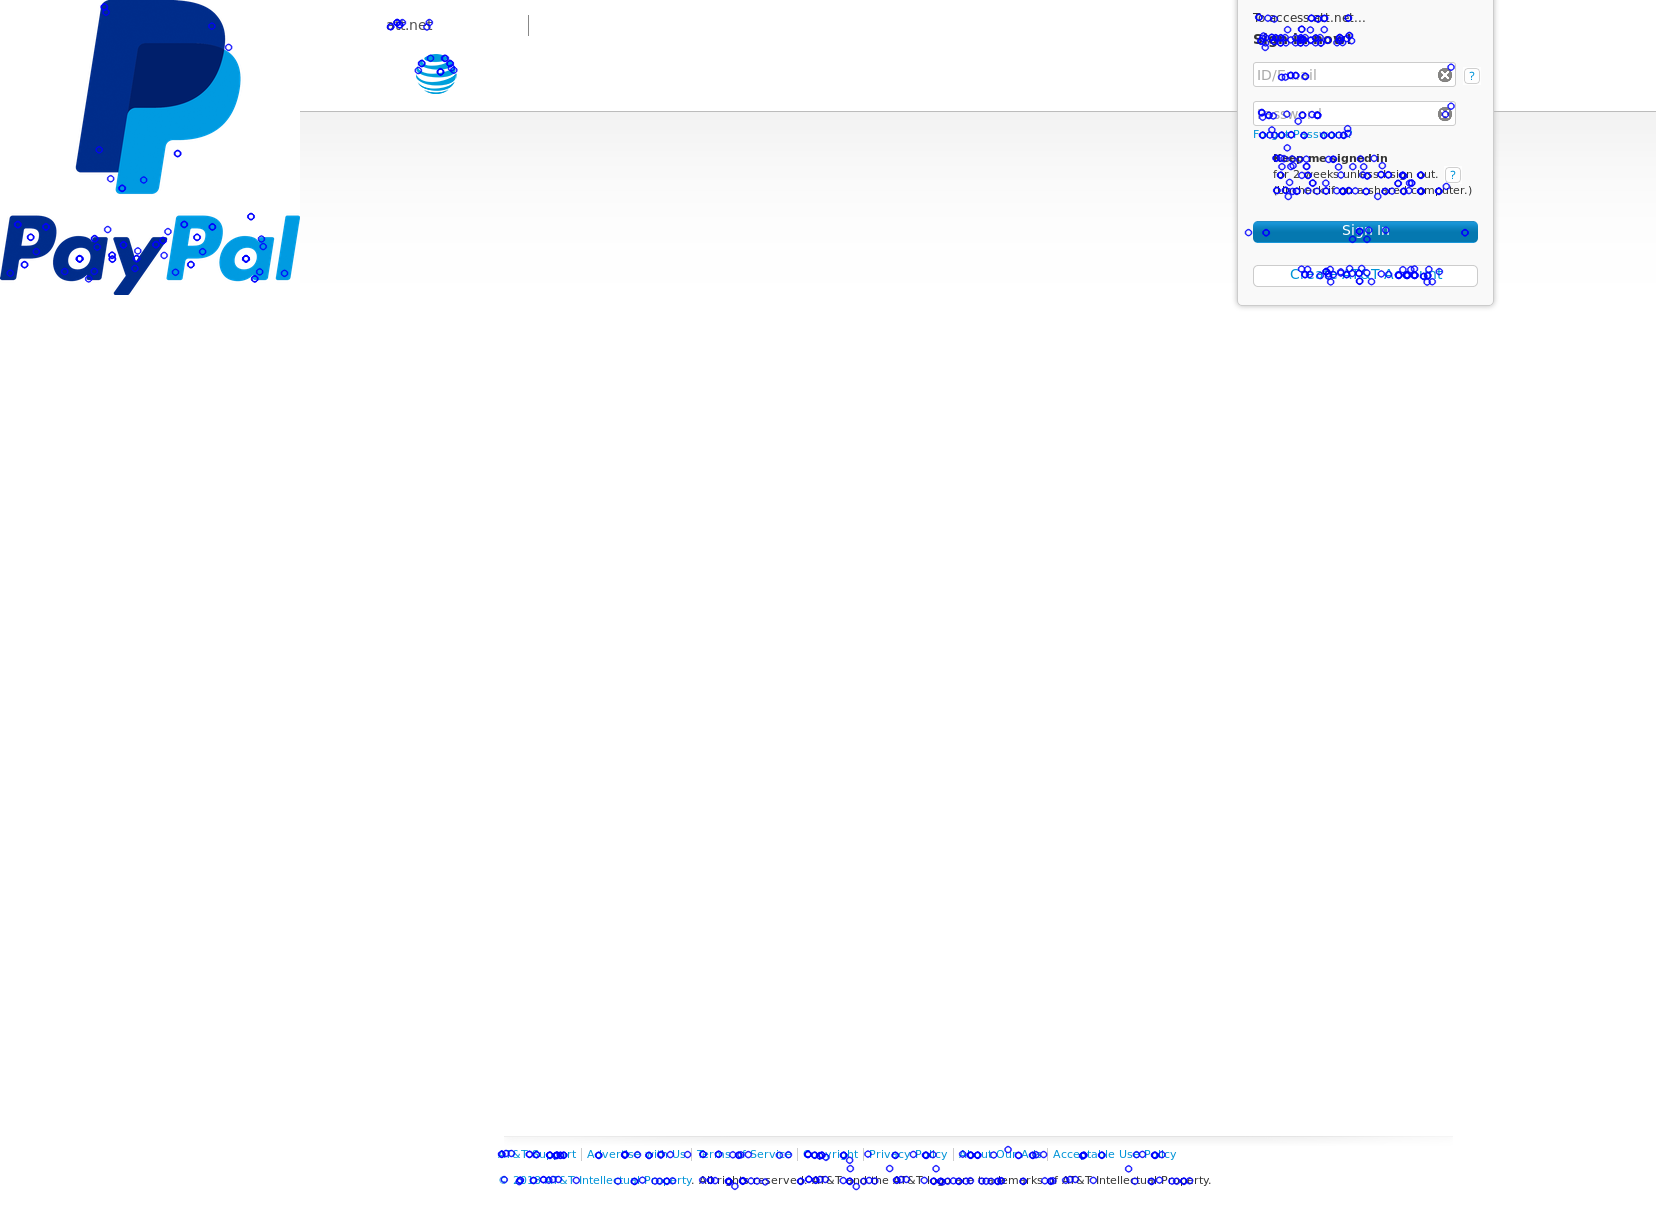
\includegraphics[width=\linewidth]{images/flannmatchingpaypal.png}}
      \\\\
      \fbox{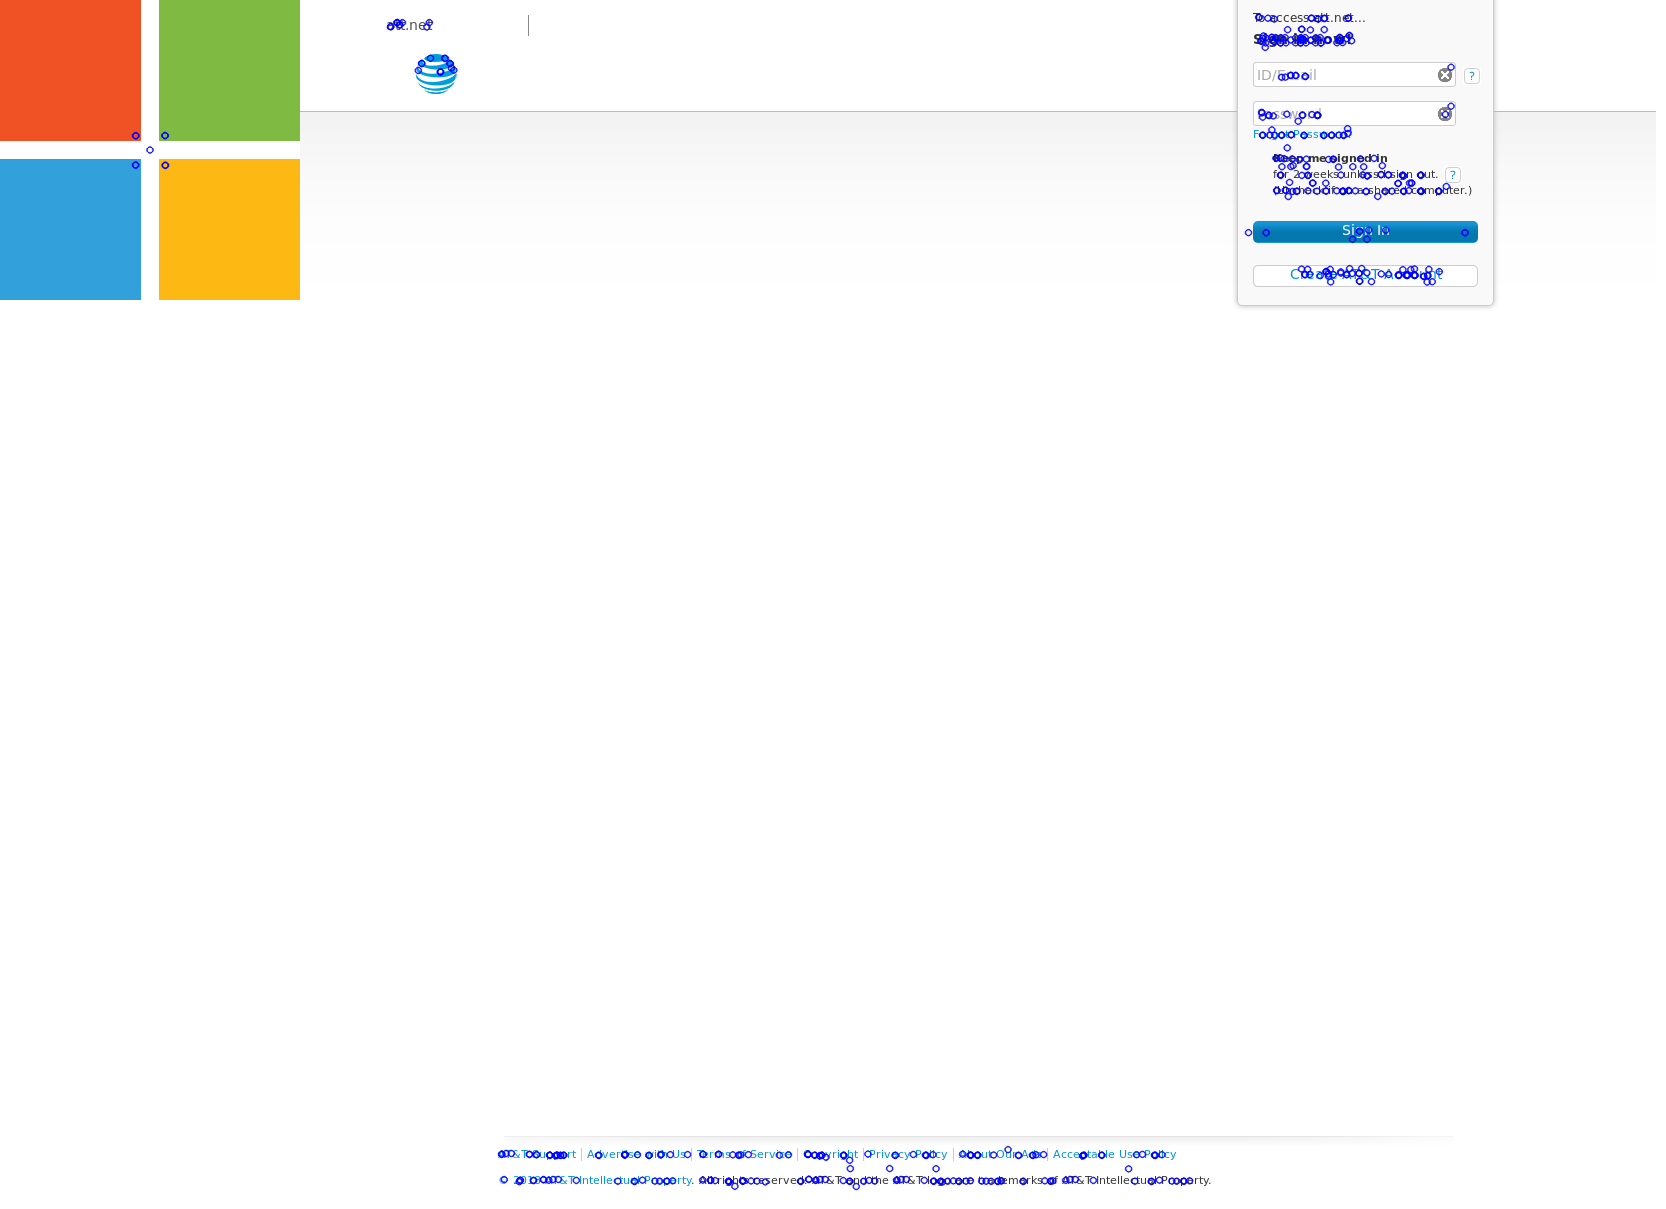
\includegraphics[width=\linewidth]{images/flannmatchingmicrosoft.png}}
    \endminipage
\end{center}
\caption{Comparison of FLANN matching with AT\&T, PayPal and Microsoft logos on AT\&T phishing page}\label{fig:flannmatchingcomparison}
\end{figure}
\restoregeometry
\newgeometry{margin = 0.7in}
\begin{figure}[!h]
\begin{center}
    \minipage{0.61\textwidth}
      \fbox{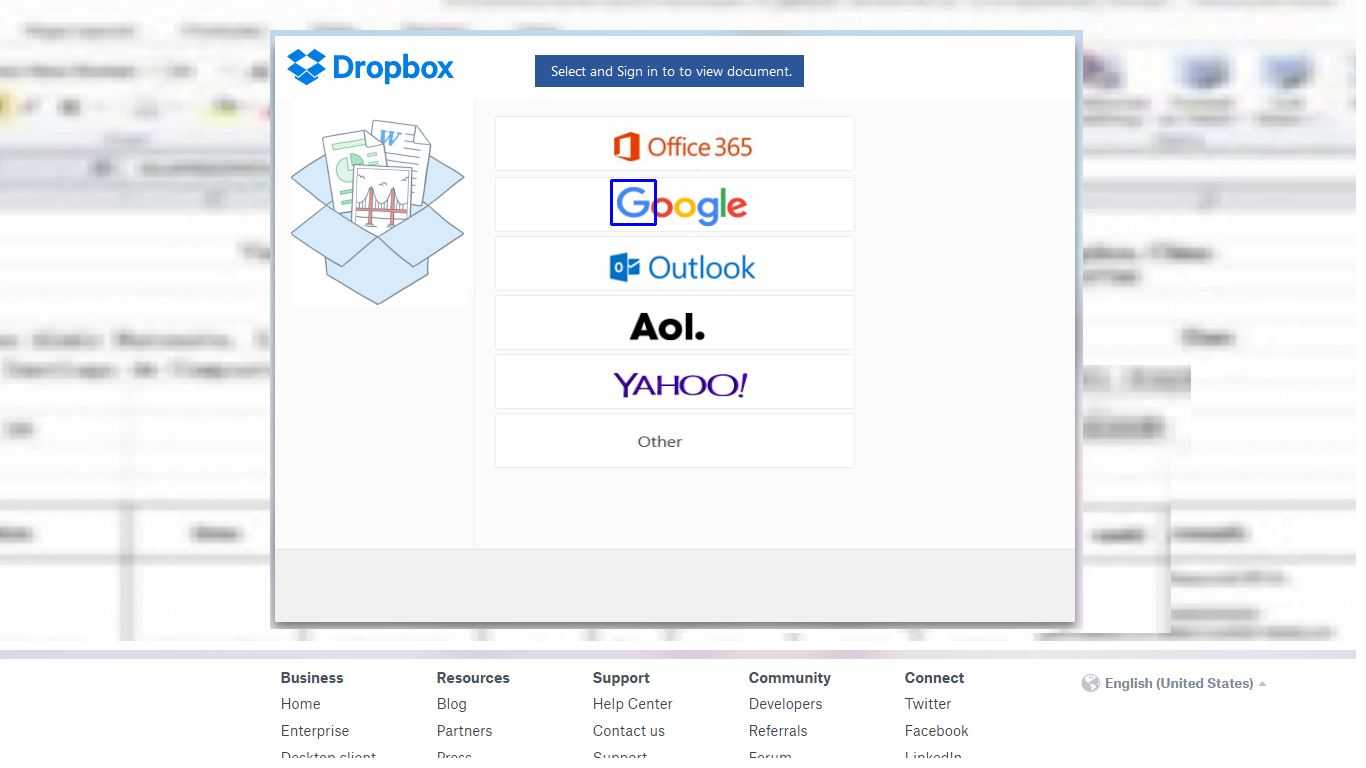
\includegraphics[width=\linewidth]{images/cascadematchinggoogle.png}}
      \\\\
      \fbox{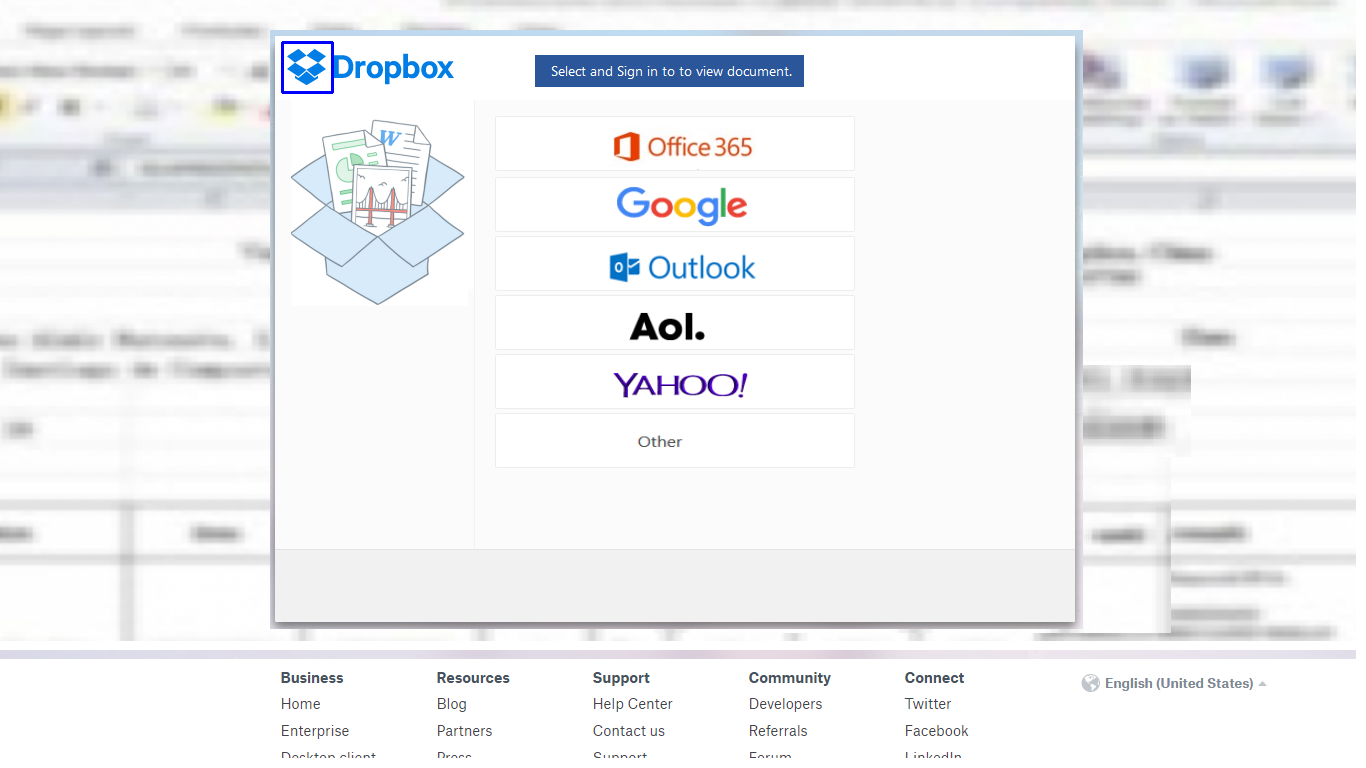
\includegraphics[width=\linewidth]{images/cascadematchingdropbox.png}}
      \\\\
      \fbox{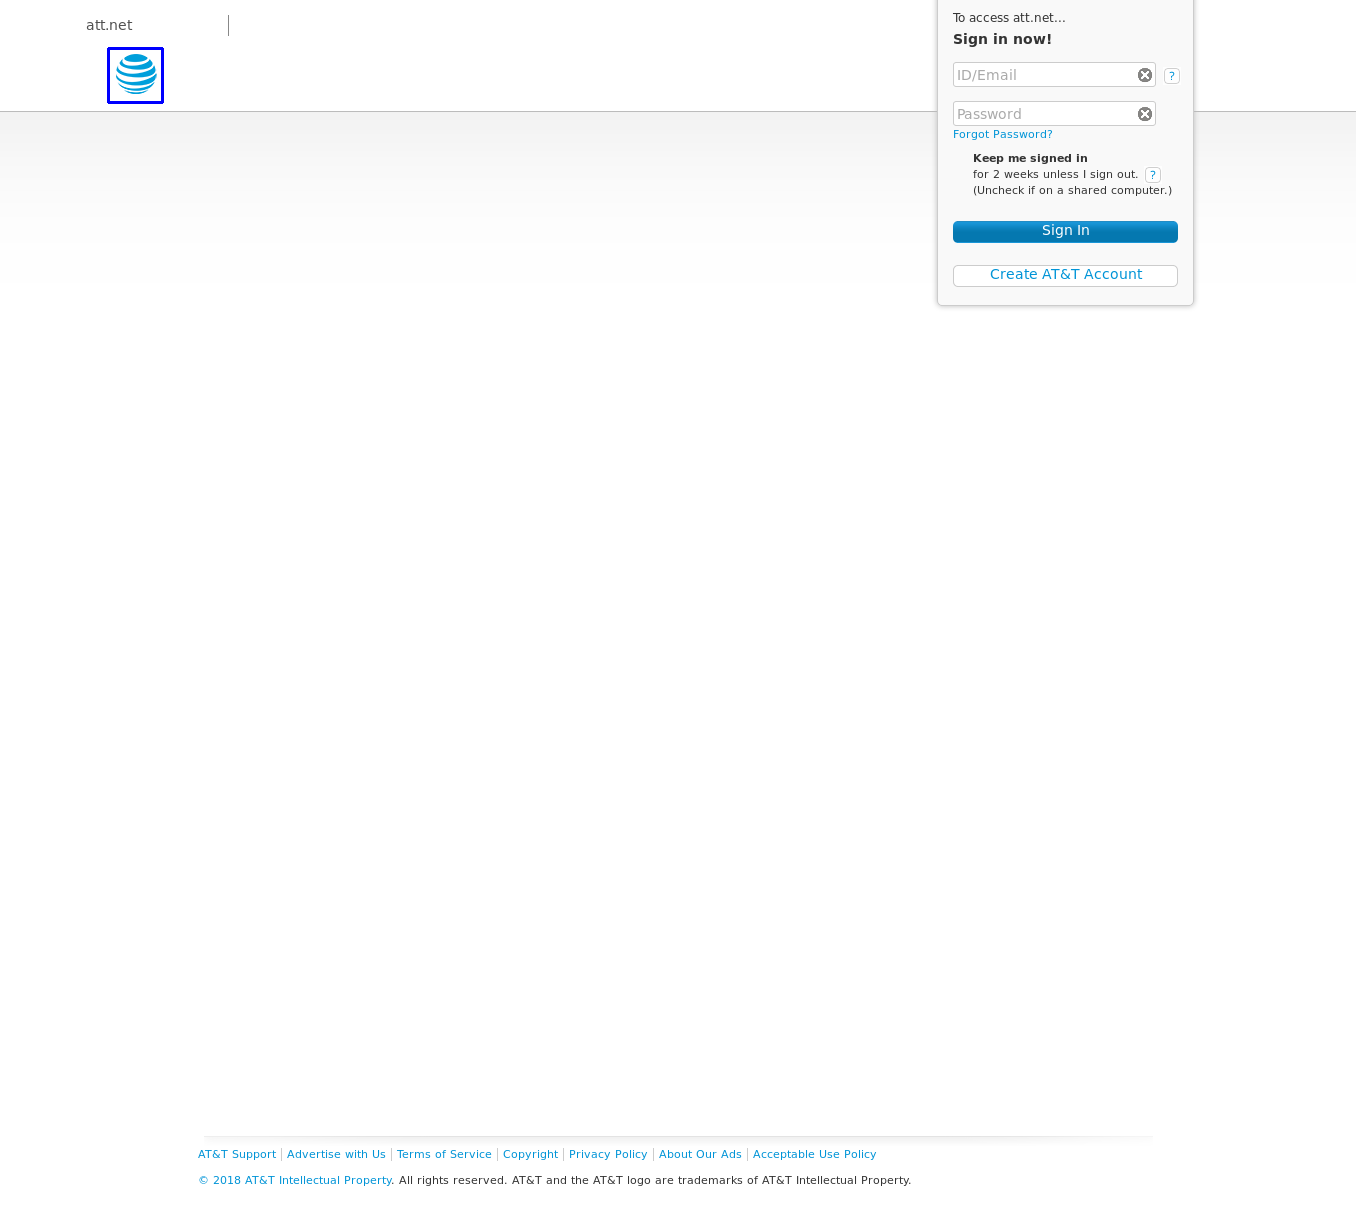
\includegraphics[width=\linewidth]{images/cascadematchingat&t.png}}
    \endminipage
\end{center}
\caption{Successful cascade matching with Dropbox AT\&T and Google logos}\label{fig:cascadematchingcomparison}
\end{figure}
\restoregeometry
\begin{figure}
    \centering
    \fbox{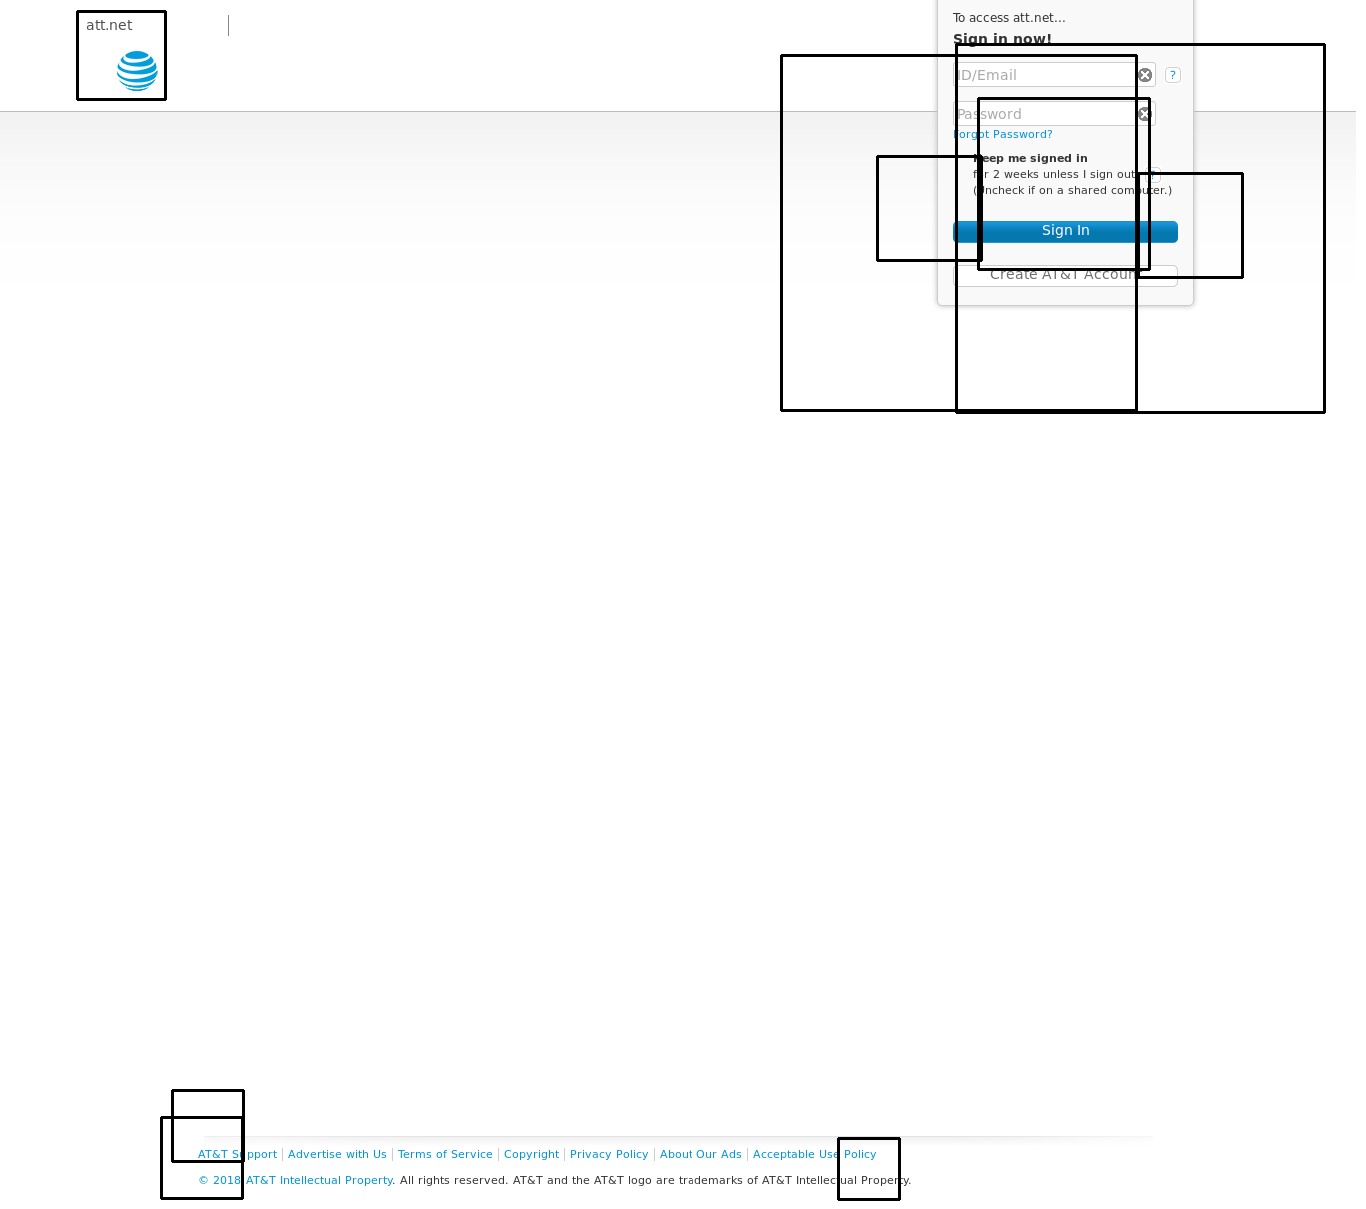
\includegraphics[width=0.59\linewidth]{images/cascadematchingnetflix.png}}
\caption{Issues with cascade trained on Netflix logo with AT\&T phishing page}\label{fig:cascadematchingnetflix}
\end{figure}
\noindent
In addition to the issues with cascades which were not working very well, such as the Netflix logo, we noticed a large number of false positives which were much harder to avoid. The logos were being identified on the page by patterns which appeared to be very similar to stylistic elements of the logo, however they were not the actual logo. We can see some of these issues in figure \ref{cascadecorrectissues}.
\\\\
We realised that, when the logo was correctly identified on the page, the bounding box of the matched image would contain pixels and colours which were similar to the logo we were matching and when the match was fitting on styles, it would sometimes be very different colours. We decided that, to add a further check with the matched area whether it was in-fact the logo or not would be sufficient. For this reason, we extracted the portions of the screenshot which had been detected by the logo and attempted to match them with the logo. We re-sized them in order to make them the same dimensions as the logo, flattened both 2-dimensional images into 1-dimensional and then applied the \texttt{compare\_ssim} function from scikit-image to compare them. We achieved a high accuracy second layer of match filtering by accepting if the \texttt{compare\_ssim} function returned a negative value.
\newgeometry{margin = 0.7in}
\begin{figure}[!h]
\begin{center}
    \minipage{0.6\textwidth}
      \fbox{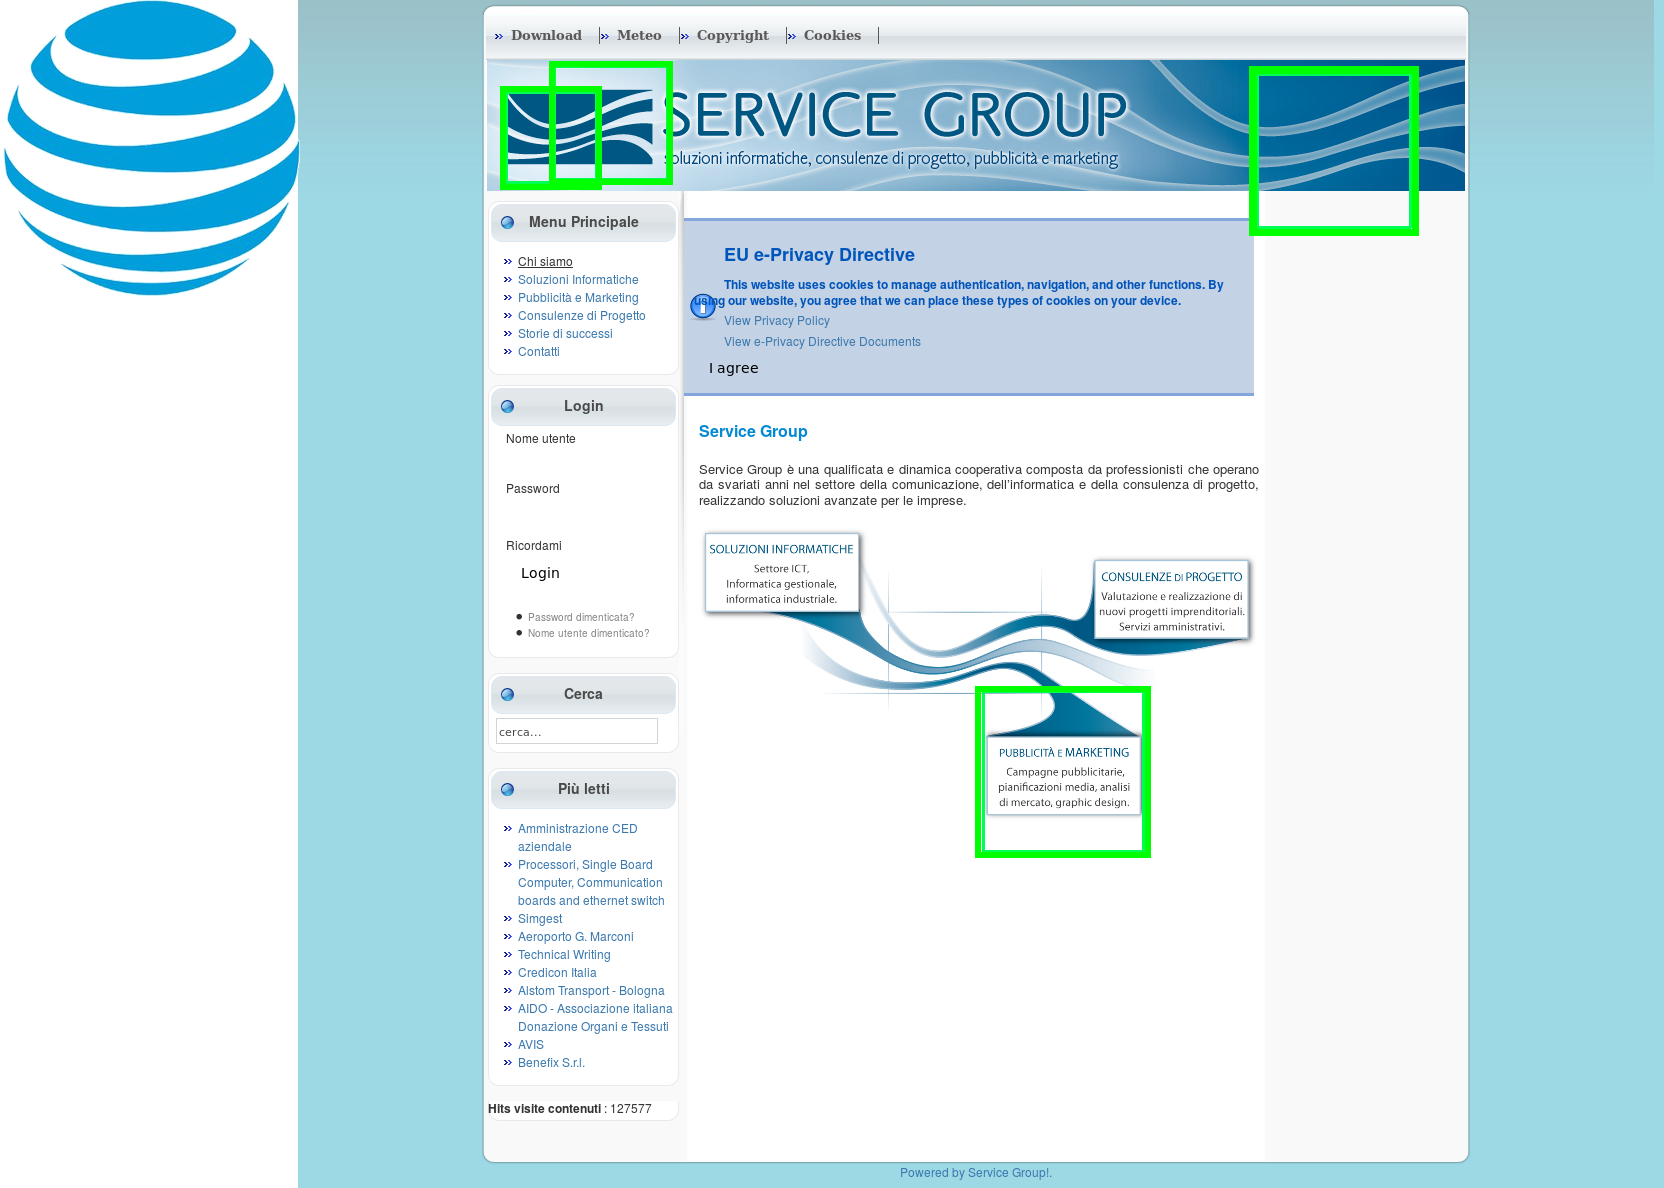
\includegraphics[width=\linewidth]{images/cascadecorrect_att1.png}}
      \\\\
      \fbox{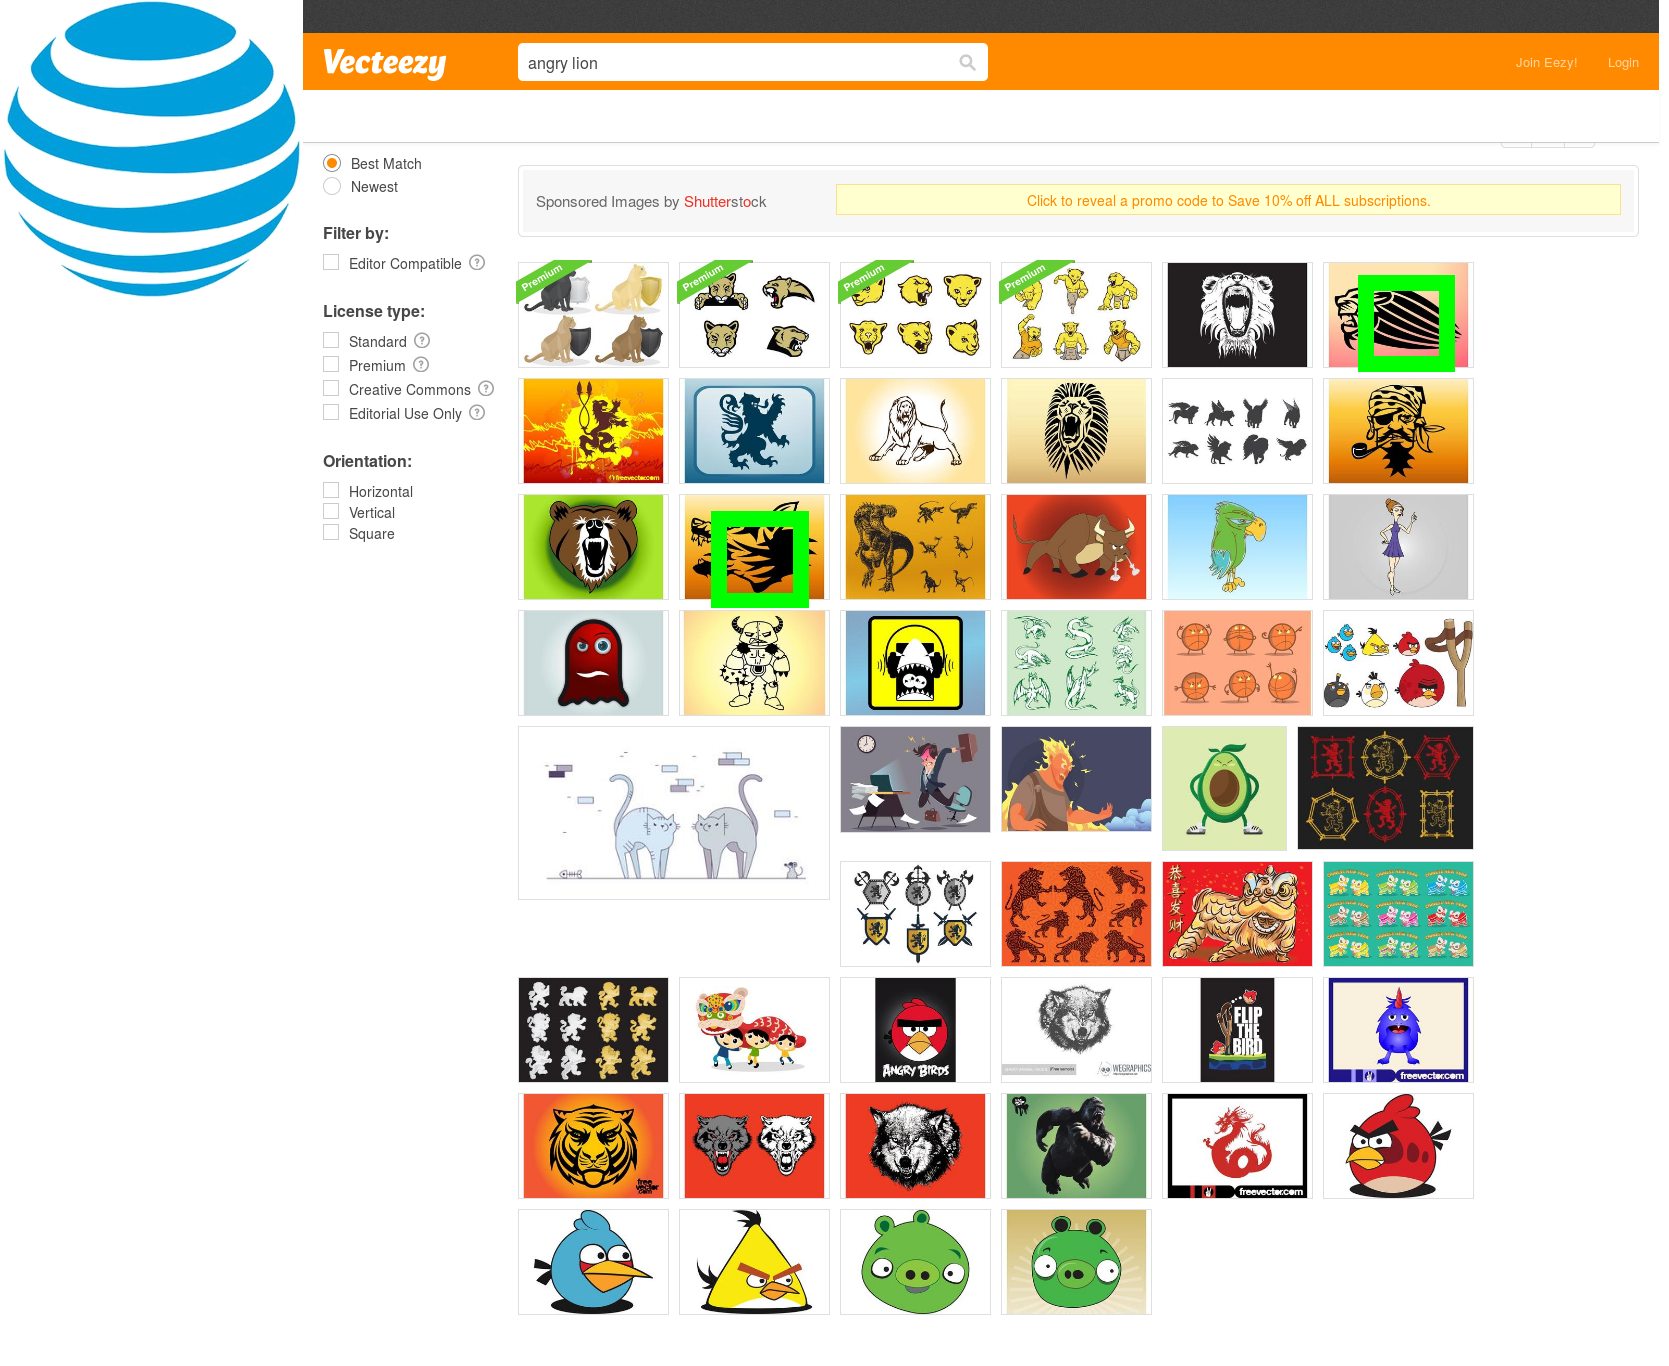
\includegraphics[width=\linewidth]{images/cascadecorrect_att.png}}
      \\\\
      \fbox{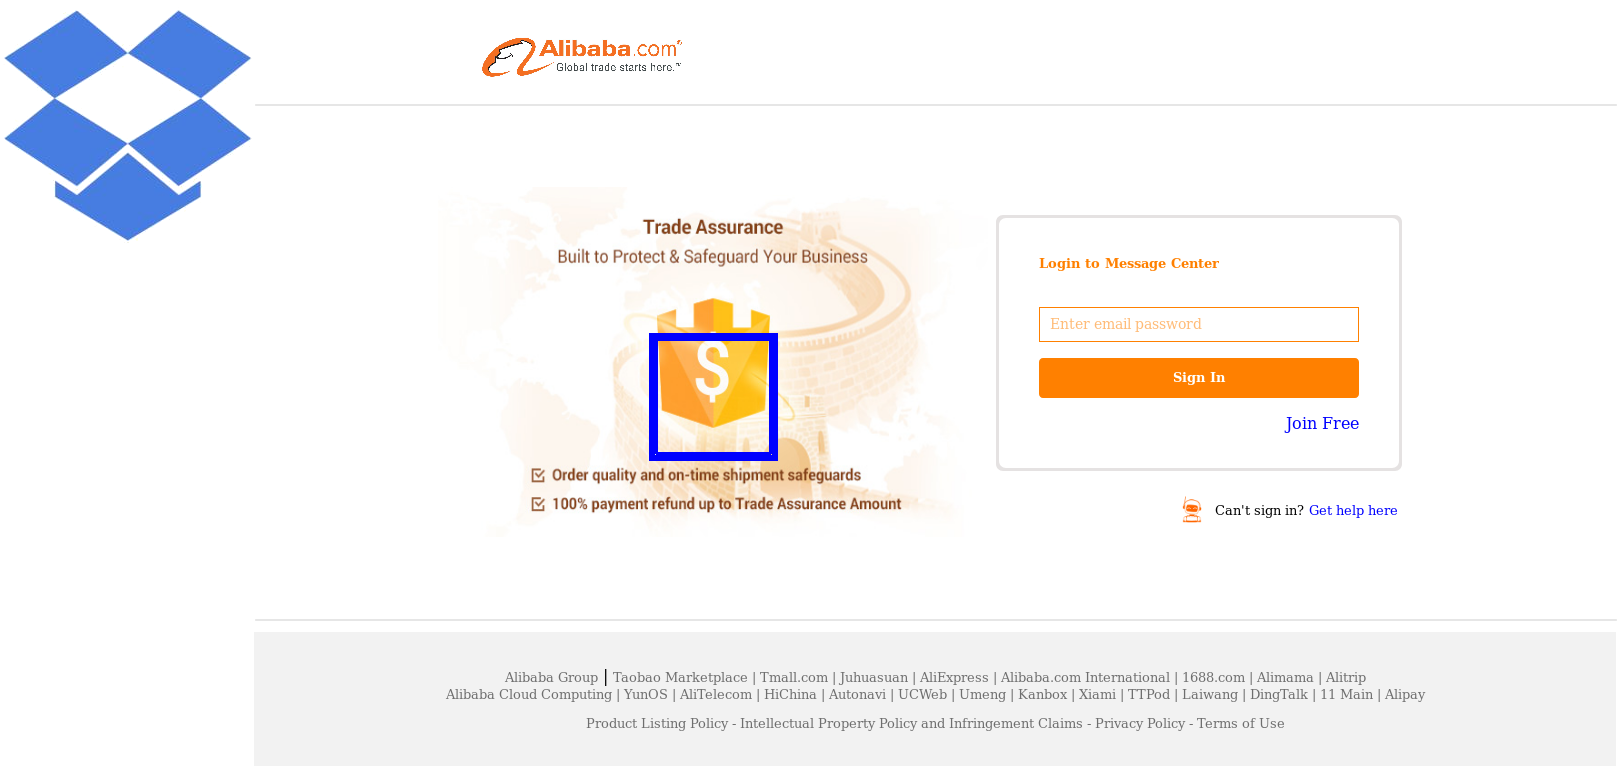
\includegraphics[width=\linewidth]{images/cascadecorrect_dropbox.png}}
    \endminipage
\end{center}
\caption{Issues with cascade matching of logos matching with patterns on the page but not of the target logo}\label{cascadecorrectissues}
\end{figure}
\restoregeometry
\clearpage
\subsection{Image Resources Vectorizer}\label{imageresourcesvectorizer}
We realised three main issues when using the screenshot vectorizer:
\begin{itemize}
    \item Not all pages had screenshots which meant that we were not applying this technique on a large number of pages
    \item We had to crop these pages for performance so we were losing potential information with the bottom part of the screenshots
    \item By scanning the entire page we are wasting a lot of time scanning parts of the page which would not contain any logos
\end{itemize}
To fix these issues we decided to run the cascade classifier on the image resources extracted from the WARC files. We did this because we believed that any logos which are on the page would be loaded into the page and therefore the browser would have to fetch these images manually.
\section{Client Server Architecture}
In order to avoid the overhead of fitting the pipeline to the trained model before returning a classification, we implemented a client server architecture using Flask which loads the trained model when it is started up \cite{flask}. Since the time taken to classify a WARC file is significantly less than the overhead of the client-server architecture, we allowed the list of files to be classified to be sent via JSON and a JSON object to be returned, with a mapping between the name of the WARC file and the classification which it has been given, thus allowing us to classify multiple WARC files per request.
\section{Batch Script Execution}
As with many machine learning projects, there were many long running scripts which we had to run in order to train and evaluate our classifier. We had to use many different architectures in order to run our classifier. We used external computational power in order to handle the large memory requirements of some of the intensive graphical computation and to avoid slowing down our machine during development.
\subsection{VMware EXSi}
We were provided access to the external computation cluster by Lastline. The cluster made use of a VMware EXSi hypervisor which allowed us to create virtual machines remotely and run our scripts on there \cite{vmwareexsi}. Since we were able to create our own environment, we were able to clone the development setup of Linux as we were running on our machine and then we were able to use the Python virtual environment to run our code without compatibility issues.
\subsection{SSH}
We were also able to run our computation on batch servers provided by Imperial College London. The advantage of running these on here was the large disk space allocation so we were able to copy all of our training and test data which allowed us to run batch training algorithms over the course of multiple days. We used tmux sessions in order to keep processes running in the background over SSH \cite{tmux}.
\\\\
One of the issues we encountered was transferring large files over to the batch computing cluster. We had around 40 gigabytes of training and testing data. We were able to use SSH tunnelling and the ability with RSync to partially copy files over and restart an interrupted process which allowed us to copy the files without being concerned about interruptions in internet connection or power issues \cite{rsync}.
\subsection{Super Computers}
We also employed the use of super computers to speed up some of the processes that we were running. We created a conda environment which we used to deploy our processes out to the super computer cluster \cite{conda}. There were various different queues for super computers which had better infrastructure and wall time availability but required longer wait times for the job to be run.
\section{Issues}
\subsection{HTTPS Upgrades}
During the collection of our WARC files, we submitted the URLs we collected to the LastLine sandbox to output the entire traffic capture for the session. However when website perform the HTTPS upgrade, they signal to the browser to create a new encrypted session for communication.
\\\\
For this reason, in our WARC files, all of the web traffic after the redirection in an HTTPS upgrade was encrypted and we were unable to analyse it.
\subsection{OpenCV Memory Leak}
We rely on OpenCV quite heavily for the image detection portions of our classifier \cite{opencv}. The implementation of OpenCV in Python which we use interacts with native C++ code using Cython for the performance critical code. While regular Python is good with garbage collection, there is a leak in the underlying code of OpenCV. We opened a GitHub issue at \url{https://github.com/opencv/opencv/issues/11559} but this is yet to be resolved.
\\\\
We temporarily patched this issue by manually deleting variables in Python as well as calling the garbage collector using the function \texttt{gc.collect()} to free the memory, however this problem did sometimes still occur on our personal development box. For this reason, we had to also use the external computing cluster sometimes with greater RAM resources to work around the memory leak until it is fixed by OpenCV.
\newpage
\chapter{Evaluation}
In this section we will discuss the performance and accuracy of our classifier and compare it against other related work in the field.
\section{URL Collection}
URL collection is one of the most common areas where bias can be brought into a machine learning model. For the malicious URL collection that we performed, we believe that the main issue was that we were learning over already classified examples. Since we were constantly polling a set of sources from researchers in the field, a lot of the pages we classify have already been marked by other automated classifiers. For this reason, we may be training and testing our model on pages which have stronger features than some of the more difficult pages to classify.
\\\\
For the benign data collection there are also potential issues with introducing bias in the popularity of the pages. The Alexa list is a descending list of the most popular pages on the internet, when we take the top 1 million list we are considering only pages which are popular on the internet \cite{alexa}. We also have no guarantees that these pages are truly legitimate, there is a possibility that pages which are malicious may be successful enough to be in the Alexa top 1 million; however we believe this to be unlikely. Also the bias of pages outside of the top 1 million is not a huge concern to us as we are more interested in classifying examples from daily user traffic which will tend to be on popular pages.
\\\\
The submission of pages to the Lastline sandbox in order to be classified can also bring about some further bias in the data. The browser and operating system will be included in the user agent and may cause the page to act differently with regards to this. We also introduce a temporal element since we performed the data collection over a period of 6 weeks, interspersed with gaps, where no data was collected. For the benign data we were constantly running freshly detected phishing pages which reduced the risk of them already being taken down. However for the benign pages, they were collected from the latest archive of crawl data in March 2018, and the capture was done during the same 6 week period during May 2018, by extracting the URLs and submitting them to Lastline's sandbox.
\\\\
R. Gowtham et al, a well cited machine learning approach to phishing classification used similar methods for URL collection, using lists of popular pages from Google, Netcraft and Alexa for their benign page collection and Phishtank, Millersmile and Reasonable-Phishing Webpages List for their malicious collection \cite{effaciousarchitecture}.
\\\\
In addition, H. Zuhair et al created a respected literature review of machine learning methods to tackle phishing classification in November 2017 \cite{issuesandperspectives}. This can be seen in figure \ref{fig:comparisontable}. From this we can see that all of the most popular phishing classifiers use similar methods for URL collection. For this reason, although our methods may introduce biases, we believe they are the best methods available today for URL collection.
\begin{figure}
    \centering
    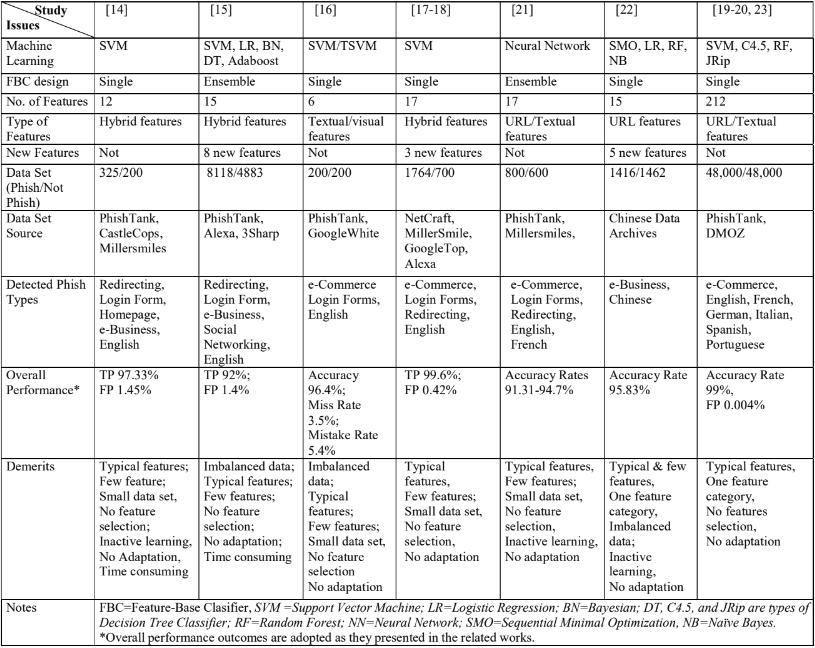
\includegraphics[width=\linewidth]{images/comparisontable.png}
    \caption{Comparison of various machine learning approaches to phishing in the literature today \cite{issuesandperspectives}}
    \label{fig:comparisontable}
\end{figure}
\clearpage
\section{Data Structure}
After ingesting the WARC files during our data loading process, we obtained the data splits as seen in \ref{fig:datastructure}. We split the data set by allocating them based on the first character of the hashed name of the WARC files.
\\\\
In total our test set is 23.04\% of our complete data set. We also had a larger proportion of our data set as malicious than benign. The proportion of our test data set which was malicious files was 71.80\% compared to 63.77\% for our test set.
\\
\begin{figure}[h]
    \centering
    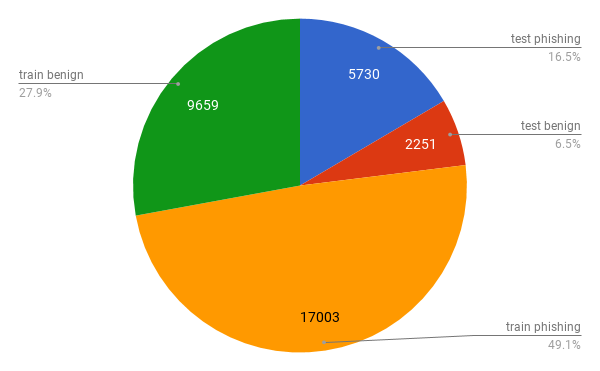
\includegraphics[width=0.8\linewidth]{images/datastructure.png}
    \caption{Distribution of our ingested benign and phishing WARC data into test and train splits}
    \label{fig:datastructure}
\end{figure}
\section{Ensemble Selection}
In order to select which ensemble we wanted to use, we had to keep the default parameters in our classifier and test our model against the three main types, the results can be seen in figure \ref{fig:rocmultipleensembles}.
\\\\
As we can see, Random Forest is by far the best ensemble for our data. We believe this is because there are various distinct feature sets for which separate decision trees are much better suited. Since we have a large feature set, ensembles like logistic regression would find it difficult find a line of best fit through all of the points.
\begin{figure}[h]
    \centering
    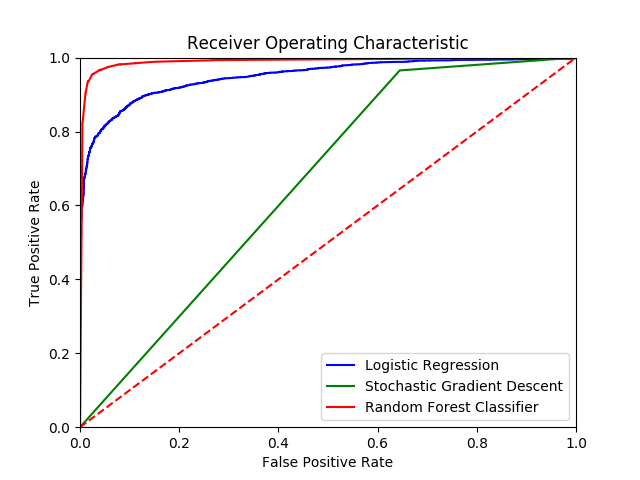
\includegraphics[width=0.6\linewidth]{images/ROC_multiple_ensembles.png}
    \caption{ROC curve displaying the relative accuracy of the three main ensembles with our classifier}
    \label{fig:rocmultipleensembles}
\end{figure}
\section{N-Grams}
We use two N-grams in our project, one for the URL and one for the body of the page. Typically one would select a value of N=2 or N=3. Since there are 256 ASCII characters, in a 2-gram, the maximal number of features would be $256^2 = 65536$ whereas with a 3-gram it is $256^3 = 16777216$.
\\\\
For this reason it was important to verify which value of N was appropriate. If we chose N=3 we would gain more information however we would have a very large feature set which could lead to over-fitting as well as a longer classification time. As can be seen in figure \ref{fig:roc_approaches}, the 3-grams gained a slight information gain on the 2-grams however they took far longer to classify and combined with the other features in our classifier we were afraid of overfitting with too many features.
\begin{figure}
    \minipage{0.5\textwidth}
      \fbox{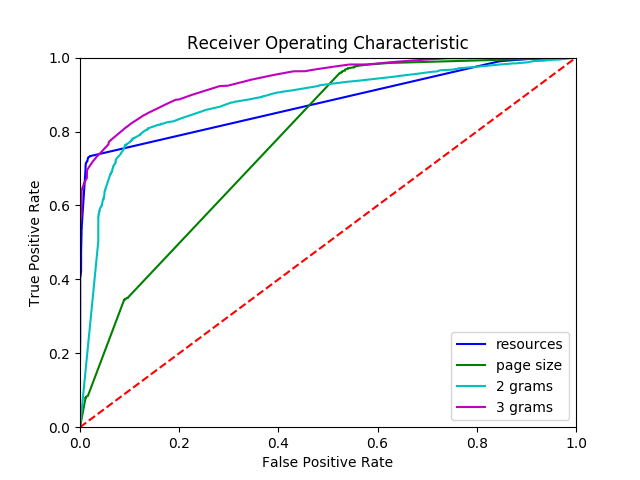
\includegraphics[width=0.9\linewidth]{images/ROC_multiple_approaches1.png}}
    \endminipage
    \minipage{0.5\textwidth}
      \fbox{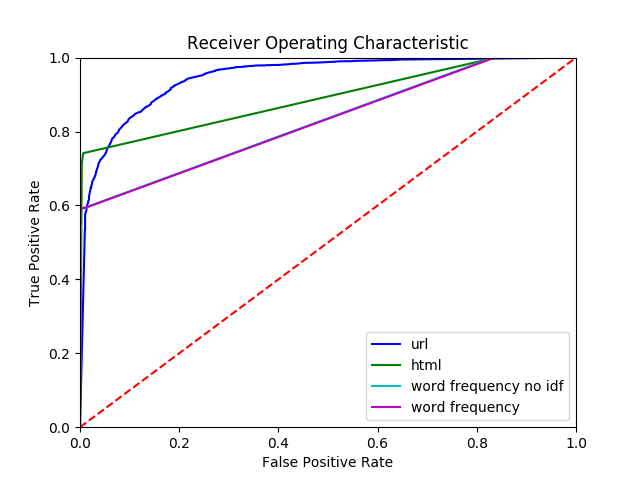
\includegraphics[width=0.9\linewidth]{images/ROC_multiple_approaches.png}}
    \endminipage
    \caption{ROC curves displaying the information gain from each of the feature extractors in our classifier}
    \label{fig:roc_approaches}
\end{figure}
\\
\section{Word Frequency}
For the word frequency vectorizer, we evaluated how well it worked in our classifier with and without using the IDF part of the TF-IDF algorithm as can be seen in figure \ref{fig:roc_approaches}. We did this by enabling the \texttt{no\_idf} option within the base \texttt{TfIdfVectorizer}. As we saw here, the line on the ROC curve when applying IDF and when applying TF only was exactly the same. We can ascertain from this that the computation of the IDF has no effect on the overall classifier. We can attribute this to two main potential reasons:
\begin{itemize}
    \item Usually malicious pages are small and therefore will have a small amount of textual content on the page, for this reason, the high TF words on the page will probably be the malicious words and the application of the IDF algorithm would not change the selected words.
    \item Many times, phishing pages have such a small textual content on the page if they simply have a login form, that all of the words on the page will be submitted to the classifier for analysis and none of the words will be ignored due to the low IDF score.
\end{itemize}
\section{Logo Detection}\label{logoevaluation}
We applied logo detection in two manners, attempting to detect the logo within the screenshot of the page and attempting to detect the logo within the image resources on the page. We trained and ran our model using a Random Forest classifier with the detection in the screenshot only, and in the extracted images only, our results can be seen in figure \ref{fig:rocscreenshotimages}.
\\\\
As we can see here, we obtain a small information gain over our test set with detecting logos within screenshots but no information gain with detection of logos in extracted images. The issue we discovered during our implementation was that the logo detection system was extremely sensitive to false positives in the cascade classifier. This is because, if there is a single model within our set of logos which performs in the same way as the Netflix model shown in figure \ref{fig:cascadematchingnetflix}, then every page would have the Netflix logo detected on it and none of them would actually derive from the Netflix hostname. This would cause the feature values for the screenshot detection to be the same for each example in our data set and the classifier would be unable to learn any information. We attempted to rectify for this by only including a few, well verified logos within our classifier during the evaluation of these components.
\\\\
This leads us onto the second potential issue with this method. Having very few trained models of our logos within our classifier caused issues. To work the best, the classifier needs an exhaustive list of trained cascades for all logos that may appear in certain pages. If any logo is detected, the classifier then checks if the hostname corresponds to the expected hostname of the logo in question. If however, we manage to detect logos in the page without actually detecting the logo of the main page then we would provide a classification leaning toward a malicious page when the page is in fact benign. In figure \ref{fig:malicious196} our classifier detected logos situated within the social media buttons on the page but did not detect the main BBC logo and the page was therefore misclassified as malicious.
\\\\
The other main issue which we tried to correct for during the implementation of this classifier in section \ref{screenshotvectorizer} was that the cascades would match on similar patterns which occurred within the screenshots of the page which did not correlate to the logo in question. We tried to correct this by doing a further comparison with the colours of the logo and the colours in the matched portion of the page which worked well however we still had false positives when the colours also happened to coincide with the logo.
\\\\
Overall, we believe that the module has a lot of potential to be an extremely strong metric as we have proven in the various positive examples shown in the implementation. Unfortunately, due to time constraints of the project, we were unable to try and solve the issues that still remain with the module, and its high sensitivity to false positives means that it did not produce desirable results. 
\begin{figure}
    \centering
    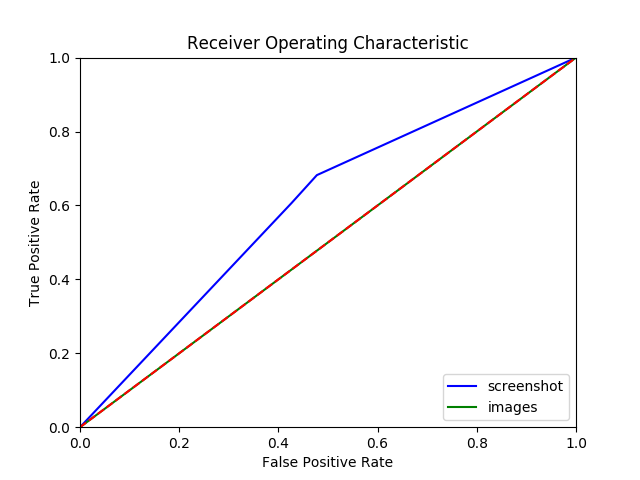
\includegraphics[width=0.6\linewidth]{images/ROC_screenshotimages.png}
    \caption{Comparison of the performance of detection of logos within the screenshot and the extracted images in our classifier}
    \label{fig:rocscreenshotimages}
\end{figure}
\section{Feature Importance}
In order to evaluate which features in our classifier are the most important, we are able to obtain the information gain that each feature has in the classifier. The results are shown in appendix \ref{appendix:featureimportance}. It is important to note that, due to the large feature set that the n-grams produce and the fact that these features would not be easy to analyse, we have not included the n-grams in our feature importance table.
\\\\
As we can see, most of the information gain that we obtain is with static analysis of the URL, status and the HTML. We saw some information gain from the logo detection methodologies in the screenshot but no information gain over the training set for the logo detection within the extracted images. It is evident that, if, even with the small number of logos and the issues we faced with the component as described in section \ref{logoevaluation}, we were able to gain a feature which performs better than some of the other features we have, then when the issues are solved, it could be a very strong feature.
\\\\
Surprisingly, one of the highest variance features in our classifier is the page height. This was a very simple metric but it proves our theory that phishing pages are generally short as compared to non-phishing pages which may be longer. We also have many of the other well-known features from the literature which attain high importance. In addition to this we gain high importance with features from the resource vectorizer we proposed ourselves.
\\\\
We also saw zero variance for many of the status numbers, this is to be expected, because even some of the common status numbers may have no bearing on whether the page is malicious or not. This may also be down to statistical bias which we obtain from our URL collection, since the crawl data and phishing sources would not submit results with the other status numbers such as a 500 server error. These codes are also less common with popular domains which have development teams to ensure their pages are always active.
\section{Classification Rate}
Our classification results for our classifier over the test set are displayed in table \ref{table:ourconfusionmatrix}. As we can see here, we are achieving an accuracy of 96.50\%. We can also see that the false positive rate with respect to the number of pages classified as phishing and the false negative rate with respect to the number of pages classified as non-phishing are similar. 
\\\\
Also, from the ROC curve for our classifier in figure \ref{fig:roc}, we can see that we obtain an extremely high true positive rate for a false positive rate of 0.05 and for a false positive rate of 0.20 we have obtained a true positive rate of almost 1.0. However, we only reach a true positive rate of 1.0 with a false positive rate of around 0.6.
\begin{table}[h]
\begin{center}
\begin{tabular}{l|l|c|c|c}
\multicolumn{2}{c}{}&\multicolumn{2}{c}{Test result}&\\
\cline{3-4}
\multicolumn{2}{c|}{}&Non-phishing&Phishing\\
\cline{2-4}
\multirow{2}{*}{True classification}& Non-phishing & $2159$ & $92$\\
\cline{2-4}
& Phishing & $187$ & $5543$\\
\cline{2-4}
\end{tabular}
\end{center}
\caption{Performance of our classifier over our test set}
\label{table:ourconfusionmatrix}
\end{table}
\begin{figure}
    \minipage{0.5\textwidth}
      \fbox{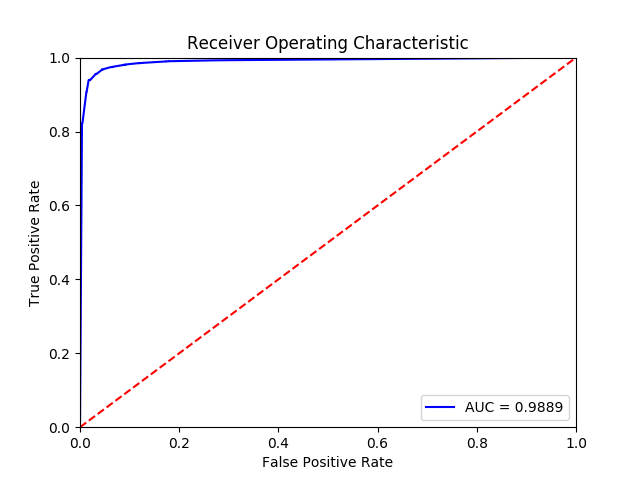
\includegraphics[width=0.9\linewidth]{images/ROC_zoomed_out.png}}
    \endminipage
    \minipage{0.5\textwidth}
      \fbox{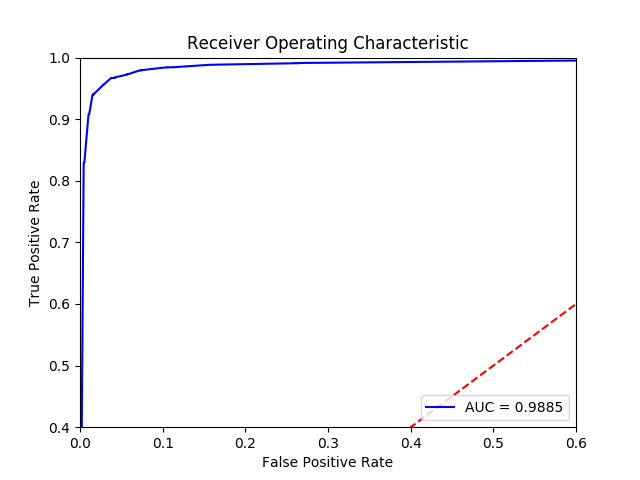
\includegraphics[width=0.9\linewidth]{images/ROC_zoomed_in.png}}
    \endminipage
    \caption{Full and zoomed in images of the ROC curve of our classifier.}
    \label{fig:roc}
\end{figure}
\\
\section{Performance Evaluation}
Performance was a big consideration in the project. As discussed in section \ref{logoevaluation}, analysing the logo in the image resources rather than the screenshot saw a marked improvement in the performance of the overall classifier. 
\\\\
Model training is something that will be performed weekly, the time to train will be similar to the time to classify for each training example. We also have an initial overhead when classifying for communicating with the server, for this reason we allowed an array of WARC files to be submitted to the server, returning an array of classifications for each file.
\\\\
Our current classifier takes on average 0.35 seconds per example to train and 2.5 seconds for each query to the server. We also have an overhead of initialising the OpenCV module which takes approximately 30 seconds to initialise however this overhead does not exist for subsequent queries in the same session \cite{opencv}.
\section{Comparison with Current Methods}
Proofpoint Emerging Threats is a leader in open source and commercial malware detection \cite{emergingthreats}. They have created a set of rules which allow users to identify a basic level of phishing detection very quickly over a wide range of pages \cite{phishpunch}. We ran their rules over the WARC files in our test set and obtained the confusion matrix in table \ref{table:etconfusionmatrix}.
\\\\
Safe Browsing is Google's ever growing blacklist of pages which are deemed to be malicious \cite{safebrowsing}. They provide an API for checking if a series of URLs are classified as malicious or not. The API provides 10,000 requests in a 24 hour period however they allow up to 500 URLs to be classified in a single call. For this reason they can not be used for live querying however at the end of each day we can query up to 5 million URLs. We have included the results of safe browsing on our test set in table \ref{table:safebrowsingconfusionmatrix}.
\begin{table}[h]
\begin{center}
\begin{tabular}{l|l|c|c|c}
\multicolumn{2}{c}{}&\multicolumn{2}{c}{Test result}&\\
\cline{3-4}
\multicolumn{2}{c|}{}&Non-phishing&Phishing\\
\cline{2-4}
\multirow{2}{*}{True classification}& Non-phishing & $2251$ & $0$\\
\cline{2-4}
& Phishing & $5595$ & $135$\\
\cline{2-4}
\end{tabular}
\end{center}
\caption{Performance of applying PhishPunch rules over our test set \cite{phishpunch}}
\label{table:etconfusionmatrix}
\end{table}
\clearpage
\begin{table}[h]
\begin{center}
\begin{tabular}{l|l|c|c|c}
\multicolumn{2}{c}{}&\multicolumn{2}{c}{Test result}&\\
\cline{3-4}
\multicolumn{2}{c|}{}&Non-phishing&Phishing\\
\cline{2-4}
\multirow{2}{*}{True classification}& Non-phishing & $2251$ & $0$\\
\cline{2-4}
& Phishing & $3918$ & $1812$\\
\cline{2-4}
\end{tabular}
\end{center}
\caption{Performance of querying Google Safe Browsing with our test set \cite{safebrowsing}}
\label{table:safebrowsingconfusionmatrix}
\end{table}
\noindent
As we can see with both Emerging Threats and Safe Browsing, they have zero false positives but high rates of false negative. This is because Emerging Threats find indisputable signals of phishing and Safe Browsing needs to consistently ensure that pages submitted to their blacklists are all malicious since their lists are being used as in-browser blocking for Google Chrome.
\\\\
Our classifier works better than many of the solutions that are current state of the art as seen in figure \ref{fig:comparisontable} and far better than Emerging Threats and Safe Browsing, however it does not perform the best. We do believe that due to the constraints that we had to adhere to with our classifier and by achieving better results than most of the commonly used methods in literature today, our methodology does improve the state of the art. These constraints include performance constraints as well as not having access to the DNS records of the page and inability to query a search engine such as Google.
\section{Overfitting}
One of the most common concerns in machine learning problems is overfitting. When a model is overfit, it performs well on the test set however it does not perform well when deployed live. This is mainly due to the fact that the model has become accustomed to bias when collecting the training and testing data. We used two techniques to test for overfitting in our classifier.
\subsection{K-Fold Cross Validation}
Cross validation is useful to evaluate whether the model is simply good at classifying on our test set specifically or if it is able to classify the entire data set at the same rate. This is generally good at checking whether we have spent too long trying to extract features from our misclassifications and therefore become overfit on our test set. We used k-fold cross validation with k=10. The results are shown in table \ref{tab:crossvalidation}.
\\\\
As we can see here, we are achieving fairly similar accuracy for each fold of the cross validation as we are for the results on the test set within $\pm1.5\%$. We can attribute the slight loss in accuracy for some of the rounds to the fact that each iteration in the cross validation is training on a smaller data set. Also some of the splits may contain less useful training examples, hence it is able to learn less information. Regardless, we are clearly still able to classify the rest of the data set almost as well as our test set.
\begin{table}[h]
    \centering
    \begin{longtable}{ |>{\raggedright\arraybackslash}p{0.12\textwidth}|>{\raggedright\arraybackslash}p{0.12\textwidth}|>{\raggedright\arraybackslash}p{0.12\textwidth}|>{\raggedright\arraybackslash}p{0.12\textwidth}|>{\raggedright\arraybackslash}p{0.12\textwidth}|>{\raggedright\arraybackslash}p{0.12\textwidth}| } 
        \hline
        Round & TN & FN & TP & FP & Accuracy \\
        \hline
        1 & 1100 & 86 & 2232 & 47 & 96.16\% \\
        \hline            
        2 & 1117 & 49 & 2244 & 55 & 97.00\% \\
        \hline            
        3 & 1140 & 71 & 2185 & 69 & 95.96\% \\
        \hline            
        4 & 1106 & 73 & 2218 & 67 & 95.93\% \\
        \hline            
        5 & 1123 & 75 & 2215 & 51 & 96.33\% \\
        \hline            
        6 & 1145 & 68 & 2201 & 50 & 96.57\% \\
        \hline            
        7 & 1169 & 61 & 2187 & 47 & 94.54\% \\
        \hline            
        8 & 1100 & 74 & 2215 & 75 & 95.67\% \\
        \hline            
        9 & 1141 & 96 & 2155 & 72 & 95.12\% \\
        \hline            
        10 & 1174 & 72 & 2156 & 62 & 96.08\% \\
        \hline
    \end{longtable}
    ~\\
    \caption{Result of 10-fold cross validation of our classifier over the entire data set}
    \label{tab:crossvalidation}
\end{table}
\subsection{Balance}
We also have an imbalance in our data set, our benign data set is 38.38\% of the size of our malicious set. Imbalances can cause bias within the classifier because the classifier can become too accustomed to seeing a certain proportion of the data to be a certain classification. In order to remove bias, we attempted to reduce the malicious testing and training data set to the size of the benign data set and then evaluate our model on that. We obtained the results as in table \ref{table:balanceddataset}.
\\\\
With the balanced data set, we achieved an accuracy of 96.00\%. This value falls right in line with the accuracy of the classifier with the cross validation results in table \ref{tab:crossvalidation}. For this reason we believe that we are not overfitting on imbalanced data sets.
\begin{table}[h]
\begin{center}
\begin{tabular}{l|l|c|c|c}
\multicolumn{2}{c}{}&\multicolumn{2}{c}{True classification}&\\
\cline{3-4}
\multicolumn{2}{c|}{}&Phishing&Non-phishing\\
\cline{2-4}
\multirow{2}{*}{Test result}& Phishing & $2187$ & $116$\\
\cline{2-4}
& Non-phishing & $64$ & $2135$\\
\cline{2-4}
\end{tabular}
\end{center}
\caption{Result of our classifier with a balanced data set}
\label{table:balanceddataset}
\end{table}
\section{Misclassifications}
We believe it was important to investigate which misclassifications we were getting in each iteration of the classifier. For this reason, during each run of our evaluation we stored the classification, URL, HTML and screenshots of the pages which we had misclassified. These are investigated below.
\subsection{URL}
When inspecting the URLs which had been incorrectly classified as benign, the first thing we noticed was the distinct lack of features which most malicious URLs would have. We are satisfied in this case that our classifier is correctly classifying the malicious pages which exhibit clear signs that the URL is malicious. Some examples of malicious URLs which have been misclassified are below:
\begin{itemize}
    \item \url{https://forums.neswangy.net/forumdisplay.php?f=5}
    \item \url{http://www.locarmix.com.br/plugins/content/souchkldekl}
    \item \url{https://rciinvoice.com/office/12/12/error.php}
\end{itemize}
From initial inspection of these URLs, it is very difficult to ascertain any features that make it different from a benign URL from a human perspective. We did, however find a small set of URLs in our larger misclassified set which contained features we could pick up on as below:
\begin{itemize}
    \item \url{https://eastnootropics.com/update-P.ayPal.com/}
    \item \url{https://steamcommunituy.com/1523540873090/mn4zqaprqmnyej6gvoy/ku...}
    \item \url{https://theatretech.co.za/ws/node/v3/WELLSFARGO-ACCOUNT-UPDATE.html}
\end{itemize}
These URLs had features which we had missed which we could have very easily extracted also such as 'WELLSFARGO' in the path, long URLs with 'steamcommunity' misspelt and 'paypal.com' in the path which has dots added. These features would easily be picked up if we had increased our target set to include these targets, however we did not want to do this since we would be overfitting on our test set.
\\\\
For the URLs which we had misclassified as malicious, most of these URLs did not exhibit malicious characteristics, this would suggest to us that the majority of these classifications had occurred due to issues with the other parts of the page rather than the URL analysis specifically. We did encounter a few examples which were benign URLs but had characteristics of malicious URLs, these can be seen below:
\begin{itemize}
    \item \url{https://www.usgs.gov/staff-profiles/craig-d-allen?logstash-usgs-pw\%3Apalladium_root_topics=&logstash-usgs-pw\%3Apalladium_root_publication_year_date=&sort=&page=2}
    \item \url{http://www.bbc.com/culture/story/20180312-the-racist-message-hidden-in-a-masterpiece?ocid=ww.social.link.twitter}
    \item \url{https://www.heavy-r.com/out.php?member=homemade-voyeur.com&url=http\%3A\%2F\%2Fwww.homemade-voyeur.com\%2Ftube\%2Fvideo\%2Fwaterpark-exposure-xwmYyVF9fNN.html}
\end{itemize}
All of the URLs above are very long. The first and the third URLs also heavily use percentage encoding which is very common in malicious URLs. In addition the second and third URLs contain what looks like other URLs inside the path, this is a very common tactic in malicious URLs and is probably why these have been flagged in our classifier. We also have found that a lot of the benign URLs which have been misclassified are from the adult industry such as in the third URL. The industry tend to use language which is more akin to malicious URLs in order to entice their users to click on the URL. We have included a full list of misclassified URLs in appendix \ref{appendix:misclassifiedurls}.
\subsection{HTML}
The vast majority of misclassified pages had no HTML code within the body of the WARC files. This is something that could be attributed to the WARC collection process. For the pages which have been incorrectly classified as benign and have HTML, we have found that the structure is usually very similar to legitimate pages.
\\\\
The HTML page for \url{http://khatsaz.com/bankofamerica.com.login.account.update/1ab5b207453ce26b2c1474c0714db8da/signInScreen.go.html} is structured very similar to a benign page. Although the page is malicious it does not have a form on the page and is not trying to obtain information from the victim. The page also has most resources retrieved from the same domain as the page is hosted on and has a small script to body ratio.
\\\\
A page which had been misclassified as malicious is \url{http://tnaflix.com/robots.txt}. This page is simply a 301 redirect, however it is a permanent redirect so we did not immediately detect the redirected page in our WARC file. The only HTML we were able to analyse was from the redirection page. For this page we were unable to ascertain much information from the URL either so it was very difficult to classify correctly.
\subsection{Screenshot}
With screenshot detection, as discussed in the implementation section \ref{screenshotvectorizer}, we had issues with many of our logos not creating cascade models which worked well. The manual work required to obtain the target logos and editing them in addition to the time taken to train the models was also a lengthy process. For these reasons, we only created models for very few logos in our training process. This gave us low detection rates with our classifier since we only had models of a few logos which matched a small proportion of the pages.
\\\\
We also had issues with benign page misclassifications due to the screenshots. Since we do not have a complete list of logos, we had issues with the page as in figure \ref{fig:malicious196}. In this screenshot, we have the login buttons for the social media accounts but we did not have the trained model for the BBC logo in the top corner. We detected the logo, however the hostname of the target URL did not match the hostnames collected for any of the images detected within the screenshot, and the page was incorrectly classified.
\\
\begin{figure}[h]
  \begin{center}
    \fbox{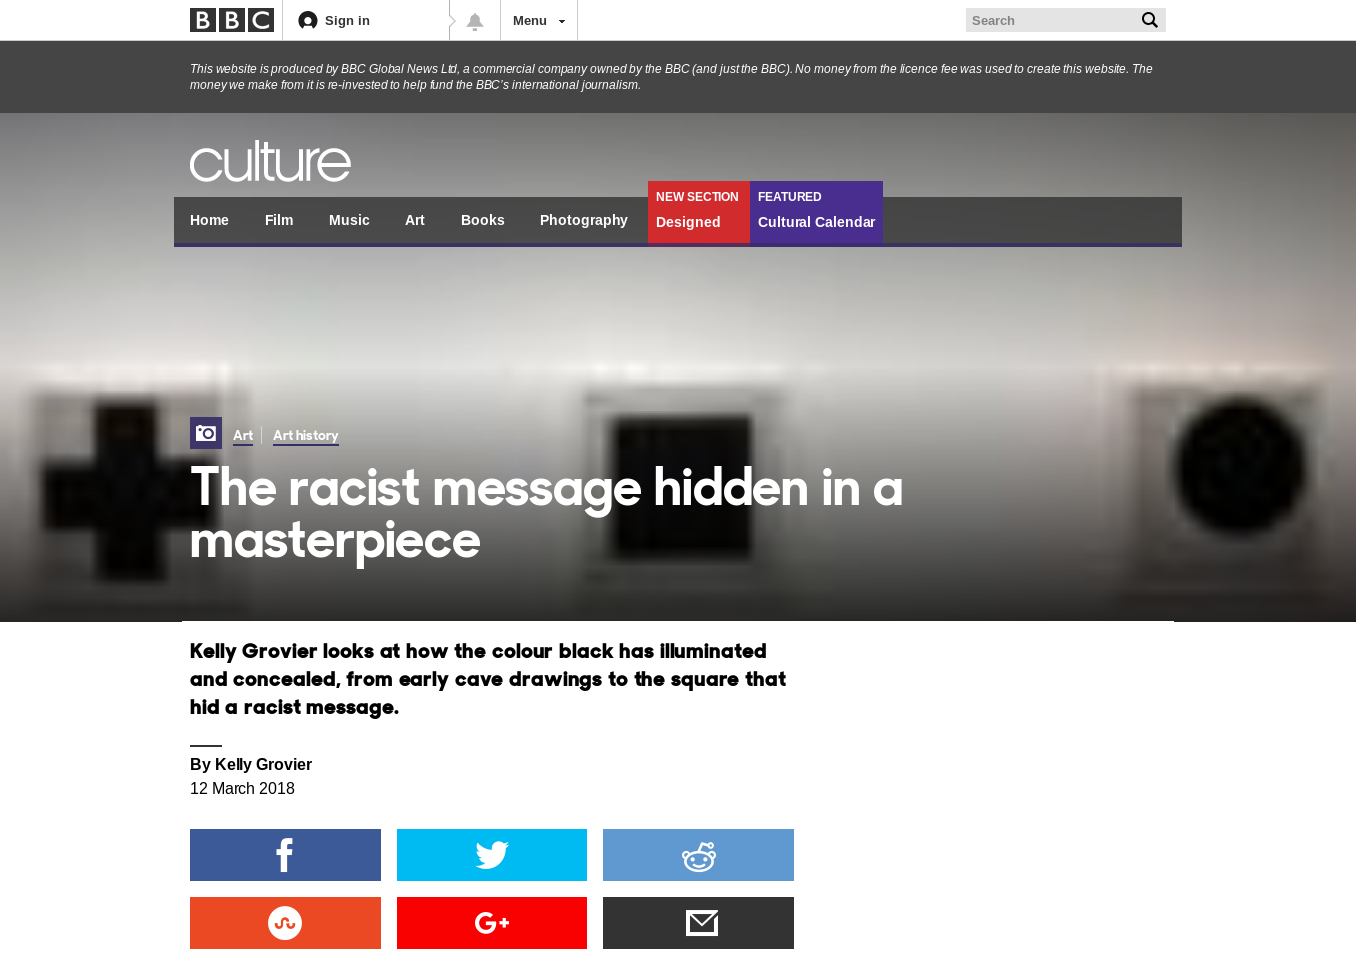
\includegraphics[width=0.69\textwidth]{images/malicious196.png}}
  \end{center}
  \caption{Example of a misclassified page where we detected the logos within the social media buttons however we did not detect the main BBC logo of the page.}
  \label{fig:malicious196}
\end{figure}
\chapter{Conclusion}
\section{Summary}
We have developed a classifier which is able to classify a page in 2.3 seconds with 96\% accuracy which falls in line with the current state of the art. We have been able to future-proof our classifier by implementing various methods such as learning the word corpus for TF-IDF directly from the training data as well as using n-grams so that the classifier can detect common letter sequences that pages use in their text as well as their URLs.  
\\\\
Further, we used computer vision methodologies in order to detect logos within web pages quickly and accurately, using methods which have not been applied before to this problem. Although we had some issues towards the end of the project with successfully integrating this functionality, we believe that given more time, we could have resolved the issues that we were facing. We have also gained confidence from the results of the classifier, that once these issues are resolved, they could accelerate the accuracy of our overall classifier to rates better than the state of the art today.
\\\\
By creating an easily extendable architecture, new methodologies can be added in order to improve the classification in the future when they are discovered. We have extracted elements from the entire page such that new modules can analyse the HTTP status, externally loaded resources, the HTML, the screenshot and the URL.
\\\\
We thoroughly evaluated our classifier and all potential biases to the point where we are confident that we are not overfitting on our data and it will continue to work well in the future to classify new pages.
\section{Future Work}
Through this research, we have been able to identify opportunities to improve the accuracy of the classification.
\subsection{Further Resource Analysis}
When we were investigating externally loaded resources from the WARC files, we analysed only PNG images which had been loaded onto the page. There are many other resources that are loaded as well such as scripts and stylesheets. In addition, these resources have information such as status codes, and which websites they are loaded, from which would be interesting to analyse.
\\\\
Through our analysis of the external resources, we found that a lot of pages which loaded images and stylesheets from external places, may often load the images directly from the target domain. It would have been interesting to be able to check as a feature, that if the logo was detected inside the image which was downloaded, whether the source of the image had matched any of the URLs which we had obtained as part of logo capture.
\subsection{Searching}
During the implementation of the first pipeline, we were achieving a lot of success when we were finding the top TF-IDF words on the page and subsequently querying Google for them. Due to the usage limitations of Google's search API and the lack of a suitable replacement where the usage allowances matched with our requirements, we believe that this could be added as a separate feature into our current pipeline again and it would help us to classify many more pages. All of the implementation for this module has already been completed, we would simply need a suitable source to query.
\clearpage
\subsection{Safe Browsing}
Google Safe Browsing has a requirement such that all URLs in their databases must be malicious, they are unable to tolerate any false positives \cite{safebrowsing}. They also have an additional advantage from ourselves that, in addition to using automated classifiers, they also use human judgement where users flag pages which they have visited and are malicious.
\\\\
For this reason it could be useful to take examples from our classifier which are marked as benign but are flagged by Safe Browsing, and then training our models with these examples. This would be useful because we would then have more training data constantly being collected at the end of each day and our classifier would be able to strengthen on the features which it is currently not identifying correctly.
\subsection{DNS Checking}
One of the things that we were unable to do in our current classifier is to check the DNS records of the pages which we were analysing. As we discussed in section \ref{hosting}, the DNS contains a lot of valuable information with regards to phishing classification, since attackers do not generally register malicious pages in the same way that legitimate pages are registered. Unfortunately, there was not a suitable API which allowed us to query this information, as well as the desire to keep all of the analysis offline, however this can easily be added as a further module in the future.
\subsection{Live Model Training}
The current structure of our classifier is that we train the model on a large data set and then we use the trained model to classify new examples. However, when the classifier is deployed, we will have various sources of confirmed pages which are legitimate or benign, either from the various phishing classification sources, from Google Safe Browsing or from the other classifiers which are deployed at the company \cite{safebrowsing}. We could develop a method where we can keep feeding our model newly classified examples and update the model on the fly rather than having to re-train over the entire data set again.
\subsection{DOM Comparison}
We did DOM comparison with our classifier in the first pipeline, however it did not work out too well due to the method of training the machine learning model. We were not able to perform direct comparisons with other DOM trees during the training, and we were forced to extract features instead. There was some initial progress, however, with offline DOM comparison between different phishing pages, and we believe that our hypothesis about DOM trees of phishing pages being closely related is true. It would be interesting if there was a way to extract the features of the DOM tree into binary features which we could input into our classifier and allow this to try and detect derivatives of other phishing kits being used.
\subsection{Automatic Logo Training}
We have already developed a method to periodically query PhishTank for the latest most popular targets of phishing attacks, automated scripts which take a target, download the top n images from Google images, and training scripts which generate the model from the logo \cite{phishtank}. The only issue which is stopping us from creating a fully automated solution for fetching logos, training their cascades, and adding their cascades to our pipeline, is the manual selection and editing of the logo to fit standards. We believe that either finding a source of plain logos which we could use, or creating a script which can automatically select and remove extra data from images and giving the images transparent backgrounds, would fully automate this portion of the pipeline as well.
\subsection{Script Analysis}
Scripts on the page, and from externally loaded files, are commonly used to track and fingerprint the way victims may use the page, as well as performing actions in the browser to convince the victim to enter their information. However, it remains a part of the page which we have not investigated yet. The only heuristics we took from the scripts currently were their size in relation to the rest of the page and HTML code. Many more features can be extracted from these and added to the classifier.
\begin{spacing}{1}
\clearpage
\pagestyle{plain}
\addcontentsline{toc}{chapter}{Bibliography}
\printbibliography
% \bibliographystyle{ieeetr}
% \bibliography{bibliography}
\clearpage
\pagestyle{mystyle}
\newgeometry{margin=0.7in}
\appendix
\chapter{Appendices}
\section{Misclassified URLs}\label{appendix:misclassifiedurls}
\begin{center}
\begin{longtable}{ |>{\raggedright\arraybackslash}p{0.75\textwidth}|>{\raggedright\arraybackslash}p{0.15\textwidth}| }
\captionsetup{width=14cm}
\hline
\textbf{URL} & \textbf{Classification}
\\
\hline
\endhead
\url{http://homesbylistorti.com/websites/2/images/Boa/19f1abc4c465912113ddocs/} & benign
\\
\hline
\url{http://www.alguaciles.cl/assets/tinymce4/js/themes/modern/DHL2016/DHL/tracking.php?} & benign
\\
\hline
\url{https://www.aryahotel.com/core/.index.html?/fpi2vw09hjogd7jhmv/} & benign
\\
\hline
\url{http://activeliving.com.au/Dropbox/} & benign
\\
\hline
\url{https://mikyc.com/wp-includes/random_compat/byte_home/Tempcontrol/} & benign
\\
\hline
\url{https://whatsmyfoodintolerance.com/blog/wp-content/plugins/pb-mium/inc/flap/ca7a4ee6eab83e5d0128ef3320996f8b/} & benign
\\
\hline
\url{https://www.kienfat.com.au/wp-content/plugins/DropNewVasion/Fresh/index.html} & benign
\\
\hline
\url{http://thegadgetisland.com/upd/Counter/index.php?email=} & benign
\\
\hline
\url{https://web.kompyte.cloud/by_timestamp/1505291139084/config/default/intermediate/https://www.nab.com.au/} & benign
\\
\hline
\url{https://valleynco.com/cgi/mail/login/} & benign
\\
\hline
\url{http://palominoroad.com/wp-content/themes/redline/lunch/cameo.php} & benign
\\
\hline
\url{http://rosemakeupartist.com/jur/image.htm} & benign
\\
\hline
\url{https://theatretech.co.za/ws/node/v3/WELLSFARGO-ACCOUNT-UPDATE.html} & benign
\\
\hline
\url{https://www.qinetwork.com.br/como-melhorar-os-processos-da-sua-empresa-com-google-docs/} & benign
\\
\hline
\url{http://jomjb.com/adobeaa/JSK/Adobe/adobeaa/9d47d25f5fa9a0d9c0b4a67949e6dd6c/index2.htm} & benign
\\
\hline
\url{https://eastnootropics.com/update-P.ayPal.com/} & benign
\\
\hline
\url{http://popodoosmartenglish.com.vn/images/class/index.html} & benign
\\
\hline
\url{https://www.yastk.com/savefiles/kutuphane/wait.html} & benign
\\
\hline
\url{https://rciinvoice.com/office/12/12/error.php} & benign
\\
\hline
\url{https://steamcommunituy.com/1523540873090/mn4zqaprqmnyej6gvoy/kujnfkdmm4j1yziya3r/lymtbeo6xartw6w1plzc/5smypbuvl87w9ufg5kd?openid.mode=checkid_setup&amp;openid.ns=http://specs.openid.net/auth/2.0&amp;openid.identity=http://specs.openid.net/auth/2.0/identifier_select&amp;openid.claimed_id=http://specs.openid.net/auth/2.0/identifier_select&amp;openid.return_to=https://skull-bets.io&amp;openid.realm=https://skull-bets.io} & benign
\\
\hline
\url{https://forums.neswangy.net/forumdisplay.php?f=5} & benign
\\
\hline
\url{https://casinodemendoza.com.ar/Amileair20018/index2.php?id=1002883B100288} & benign
\\
\hline
\url{http://web.me.com/familienholmen/hjemmesidefinalny/Forside.html/} & benign
\\
\hline
\url{https://vedredi.hu/Yah/Yahoo!/updateY!.html} & benign
\\
\hline
\url{http://steviaworld.com/downloader/js/cmd/} & benign
\\
\hline
\url{http://ow.ly/pwAk30gZWEo?verify-account-disable=notice=1} & benign
\\
\hline
\url{https://kaceauden.com/Impots/d338fca8383f1f37d191352381e94b06/} & benign
\\
\hline
\url{http://www.locarmix.com.br/plugins/content/souchkldekl} & benign
\\
\hline
\url{http://maannioda.com/graywbz/84c912c040936bf3e333d28993d87673-|84c912c040936bf3e333d28993d87673/} & benign
\\
\hline
\url{https://estaegypt.org/CitiBankAcessoSeguroInternet/BRGCB/JPS/portal/Home.do.php} & benign
\\
\hline
\url{https://files.fm/down.php?i=z6v5a2z9&amp;n=Case+ID+923-095-834-233.html} & benign
\\
\hline
\url{https://tiryakihaliyikama.net/temp/pdf-/pdf/} & benign
\\
\hline
\url{https://urldefense.proofpoint.com/v2/url?u=http-3A__biokamakozmetik.com_v-3Fuid-3Derik-2Djan.ottersberg-40umusic.com-26PZUBM8LXY3S8MNRZ&amp;d=DwMFaQ&amp;c=o_lJda16WK5Kq4wBheKNrA&amp;r=lnGECQZHffXEFiJUF9iYAX_YFSCcF9bNt1CqragjPjc&amp;m=sv101HcedDbfAUizN0kPibhv-e4nleyzPUD5HGoXMwI&amp;s=qUeRVVqdRKVpsAYOqs43FeL0Jb0JPy5yMIe3CCF0VBQ&amp;e=} & benign
\\
\hline
\url{http://nikoletburzynska.com/includes/cc/gade.php?https://login.srf?wa=wsignin=Xclusiv-3D|} & benign
\\
\hline
\url{http://www.tonsing.net/plugin/wp-admin/} & benign
\\
\hline
\url{https://bakerynepal.com/_cgi-bin/3RERZXE/12AQDWS/verification/6B5E4D3M75ND013939AM/etape1.html} & benign
\\
\hline
\url{http://badlands.ca/gallery2} & benign
\\
\hline
\url{http://digivoyage.com/atttttt/image.htm} & benign
\\
\hline
\url{https://www.milaon.tk/rxc/qoqdoc/} & benign
\\
\hline
\url{https://shop.kynoppe.com/media/mod_languages/css/get-help} & benign
\\
\hline
\url{http://aviatraaccelerators.org/a/} & benign
\\
\hline
\url{https://www.widoobiz.com/wp-content/themes/Widoobiz/help/assets/images/Doc/Doc/Sign/index.php} & benign
\\
\hline
\url{http://www.krush.fm/wp-includes/pomo/entry/611311b25c470c2ead3f87987f9e7d4b/} & benign
\\
\hline
\url{https://valleynco.com/wp-includes/css/mail/login/} & benign
\\
\hline
\url{https://knuppel.com.au/includes/onedrive/en-us/index.html} & benign
\\
\hline
\url{https://www.leandropacheco.adv.br/index.html} & benign
\\
\hline
\url{http://stpatricksfc.net/xs/dl/New\%20folder} & benign
\\
\hline
\url{http://aretecopiousproperties.com/bin0a00a/verification/87EC99B4C81A3AMM07DE/qes.php} & benign
\\
\hline
\url{http://www.arteenimagen.net/golden/GDD/GDD/GDD/GDD/GD.zip/} & benign
\\
\hline
\url{http://viddiflash.com/https/1/www.bbvanet.com.co/ecard/OTPresend.php} & benign
\\
\hline
\url{http://highschooldropouts.info/N7277k/Adobe.pdf/adobe.php} & benign
\\
\hline
\url{https://www.google.com/url?sa=t&amp;rct=j&amp;q=&amp;esrc=s&amp;source=web&amp;cd=10&amp;cad=rja&amp;uact=8&amp;ved=0ahUKEwjkp6GamKLZAhURZlAKHc41CoQQFghxMAk&amp;url=http\%3A\%2F\%2Fwww.soniverbags.com\%2Fnews.php&amp;usg=AOvVaw2MjQ0SSIYHGjl7kTa4CkLo} & benign
\\
\hline
\url{hthttp://www.kostow.pl//wp-admin/img/2/index.htm} & benign
\\
\hline
\url{https://puertolopez.gob.ec/wellsneh/indexxx.htm} & benign
\\
\hline
\url{https://www.kardum-partneri.hr/wp-includes/css/eorro/cn/dcedb/} & benign
\\
\hline
\url{https://gid-designferta/-/-/latest/Update.html} & benign
\\
\hline
\url{https://grayscala.com/wp-admin/includes/user-fed/navyfederalcreditunio/nav.htm} & benign
\\
\hline
\url{https://trainingrumahsakit.com/admin/DoCuSigN/DoCuSigN/index.php} & benign
\\
\hline
\url{http://bradescopj.com/html/classic/index.shtm} & benign
\\
\hline
\url{https://divyaravi.com/wp-admin/maint/index.html} & benign
\\
\hline
\url{https://www.aurinkoharju.fi/wp-includes/js/geusg/red.php} & benign
\\
\hline
\url{https://brazilairporttransfers.com/king/33771a4f4acb4a98be2e95f966da9beb/} & benign
\\
\hline
\url{http://www.importarmas.com/modules/mod_feed/Alibaba.html?id=MC1IDX1gEM--h6BmklV77yUjPz71wiS-VpYO1tv3CYQmXmLbAQz8Y5KvFCNlTWFzK6mY8aa&amp;tracelog=inquiry|view_details|100321842457&amp;biz_type=Notifications_MC&amp;crm_mtn_tracelog_task_id=176df315-8d37-4594-8315-fe46abf37aa5&amp;crm_mtn_tracelog_log_id=13641815851} & benign
\\
\hline
\url{https://t.yesware.com/tt/0b1bbdf5e8c05c6ef8f0d511bf601702d8c8e8ce/c0205025e173fa23ec343232485acd39/0e8c9124a0cd64a6d760698c3e1e390e/milehidistilling.com/how-to-make-moonshine/} & benign
\\
\hline
\url{https://cliqmedia.com.ng/wp-admin/css/colors/light/Adobe/} & benign
\\
\hline
\url{https://grupadellarte.pl/ofiuha/official/invoice/attached} & benign
\\
\hline
\url{https://www.mako-store.pl/libs/cccomwellercommmm/7d1fe9e45241664682ce78547cce5475/sec2.php} & benign
\\
\hline
\url{https://gobighub.com/.well-known/} & benign
\\
\hline
\url{https://www.theviralscene.com/wp-adm/134a0078150ea9acfb56caba2b33b33d/} & benign
\\
\hline
\url{http://bockchrain.com/wallet/#/?gclid=EAIaIQobChMIkYji8uvx1gIVDgOGCh0q_gjBEAAYASAAEgJqefD_BwE} & benign
\\
\hline
\url{https://www.cutterbuck.co.za/wp-admin/css/colors/ocean/1dRive} & benign
\\
\hline
\url{https://www.gimadolciumi.com/PACK/tor/} & benign
\\
\hline
\url{http://www.elenacoello.com/Loevo-fazer} & benign
\\
\hline
\url{https://superiorasphalt.com/wp-includes/SimplePie/XML/Declaration/security_checkpoint/action.php} & benign
\\
\hline
\url{https://www.aryahotel.com/core/.index.html?/fpi2vw09hjogd7jhmv/} & benign
\\
\hline
\url{https://piscine-et-eau.fr/tmp/cm/dos/bout/particuliers/authentification/devenir/Identifiant/conseils/internet/caisses/compte/code/mutualite/Nationale/31b75/pay/ser.php} & benign
\\
\hline
\url{https://www.lawyerdivorce.co.il/wp-inclbt0h30} & benign
\\
\hline
\url{https://fingerpaintedblog.com/wp-admin/includes/wid-nav/navyfederal-credit-union/intel.htm} & benign
\\
\hline
\url{http://ittechware.com/software/} & benign
\\
\hline
\url{http://siliconebands.ca/wp-content/Gdocs/e40f487275d35fca89d8835604fece02} & benign
\\
\hline
\url{https://www.exportgrowth.com/modules/mod_roksprocket/orangee/orange/} & benign
\\
\hline
\url{http://premiumblue.net/modules/mod_simplefileuploadv1.3/elements/all/ii.htm} & benign
\\
\hline
\url{http://www.sanzay.com.br/file/QDS/adm/314345/SOS9890IMPLIFICADO2017.html} & benign
\\
\hline
\url{http://www.setarehabi.ir/AccountVerify/nsw/data/} & benign
\\
\hline
\url{http://colmetric.com/media/jui/css/doc/drive/} & benign
\\
\hline
\url{https://eskola.lk/kaka/attiinnddeexx.php} & benign
\\
\hline
\url{http://www.geotalot.com/index_files/lockedfiles/e6852b48e95e60c44482a77a0b40e31c/} & benign
\\
\hline
\url{https://kaceauden.com/Impots/119951d00a5de3f0666c120ca2c596b2/} & benign
\\
\hline
\url{http://karasserybank.com/da9c13eff2b8731f4bdf11c95d059ecbda9c13eff2b8731f4bdf11c95d059ecb/618735a7c9209dc2ecdc8a22b793d39a618735a7c9209dc2ecdc8a22b793d39a/319c03858a4ec8cef3e03d46744fc792319c03858a4ec8cef3e03d46744fc792/Login/Login/Paypal-update/Login.php?} & benign
\\
\hline
\url{https://tkzwhdyk.com/sqrup/squareup_com/mysquare/a10ac55cbe09b96852ec3711ca3ef250/email.php} & benign
\\
\hline
\url{http://allmobil.com/themes/welp/customer_center/customer-IDPP00C148/2b0537b75ed9df40ce093c3e94a08d37/} & benign
\\
\hline
\url{http://hormontant.se/wp-includes/css/picuter/www.pnc/page/verification/online/1/index.html} & benign
\\
\hline
\url{http://bradescopj.com/html/classic/index.shtm} & benign
\\
\hline
\url{https://www.standardintlbank.com/.redd/js.htm} & benign
\\
\hline
\url{https://www.zipsurvey.com/Survey.aspx?suid=85067} & benign
\\
\hline
\url{http://tienda.delivery/tommmaaaa/killer/index.html} & benign
\\
\hline
\url{http://pulcrilin.net/tv5/images} & benign
\\
\hline
\url{https://www.puroslusitanos.com/wp-content/plugins/contact-form-7/zoominfo.com} & benign
\\
\hline
\url{http://www.customercarenumber.co.uk/bt-com-change-password-reset-help/} & benign
\\
\hline
\url{http://www.widoobiz.com/wp-content/themes/Widoobiz/help/assets/images/Doc/Doc/Sign/index.php} & benign
\\
\hline
\url{https://www.blueseaalex.com/m/page/match.html#/} & benign
\\
\hline
\url{http://www.iolagalerston.com/e-signatures/} & benign
\\
\hline
\url{http://tienda.delivery/tommmaaaa/killer/index.html} & benign
\\
\hline
\url{http://www.bouncewell.com/tenn//1dcad8cc5b82a7ef72f72716b220cf13} & benign
\\
\hline
\url{http://jomjb.com/adobeaa/JSK/Adobe/adobeaa/8d81541be850c565aa97631cedc8d61f/index2.htm} & benign
\\
\hline
\url{https://indogadget.web.id/wp-content/uploads/2014/06/ii.php} & benign
\\
\hline
\url{https://medicalnetgroup.com/ordstrackgmluk/} & benign
\\
\hline
\url{http://www.exmouthchapel.com/templates/exmouth2/login.php} & benign
\\
\hline
\url{http://kirbytent.com/wp-content/plugins/capability-manager-enhanced/includes/variable.php} & benign
\\
\hline
\url{https://secure.racine.ra.it/antispam/b.php?i=03Qak6pkF&amp;m=e837931158ae&amp;t=20160125&amp;c=n} & benign
\\
\hline
\url{http://www.forumactif.com/annuaire/jeux/world-of-warcraft/guilde-rp} & benign
\\
\hline
\url{https://href.li/?http://www.ebay.co.uk/itm/VERY-LARGE-STONE-ACORN-FINIAL-ANTIQUE-FINml} & benign
\\
\hline
\url{https://www.editionsadlib.com/media/news/a720351eac246fcd55c8/} & benign
\\
\hline
\url{http://allmobil.com/themes/welp/customer_center/customer-IDPP00C148/2b0537b75ed9df40ce093c3e94a08d37/} & benign
\\
\hline
\url{http://ashaimarineintl.com/content/spreadsheet/Excel_PO/New_PO016117.html} & benign
\\
\hline
\url{https://www.shakinnstirred.com/support/security/paypal-team/webapps/73274a9b20c4aaf9be60c9936e8dbfe6/CreditCard.php} & benign
\\
\hline
\url{http://www.corsiacademy.it/2010/come-si-calcola-il-valore-catastale-di-un-immobile.html} & benign
\\
\hline
\url{http://utic.espe.edu.ec/wp-content/themes/zerif-lite/ti-prevdem/img/-/css/-/com.au/big/pond/nocharge/-/-/} & benign
\\
\hline
\url{https://casahorus.com/hjd/Ourtime/ourtime.php} & benign
\\
\hline
\url{http://www.assitej.pl/wpzz/roundcube/index.html?} & benign
\\
\hline
\url{https://fullactivators.com/mac/paragon-ntfs-crack-with-keygen/} & benign
\\
\hline
\url{http://buraphwood.com/docch/source} & benign
\\
\hline
\url{http://moviepassage.com?subid=dropbox.cm} & benign
\\
\hline
\url{http://solidallianzemfb.com/sollidallianze/pdf/pdf_access.php} & benign
\\
\hline
\url{https://downuptime.net/redirect.php?url=http\%3A\%2F\%2Fdoom-audio.de\%2Fde\%2Fred.html?sec=&token=null} & benign
\\
\hline
\url{https://www.sportvsochi.ru/customer/account/} & benign
\\
\hline
\url{http://evkapen.com/in/#https://www.infomaniak.com/fr/support/payer-facturein/https://login.infomaniak.com/fr/login} & benign
\\
\hline
\url{http://gulfuniform.com.sa/chasey/activation.htm} & benign
\\
\hline
\url{https://grtrucking.net/update-wells/WellsLINK/} & benign
\\
\hline
\url{http://captainjodydonewar.com/wp-content/tnroll/Bank_Of_America/verification/7CD571B73B7655204MC7/index.php?country.x=MX-Mexico} & benign
\\
\hline
\url{https://www.gundersons.com/blog/wp-content/uploads/2016/11/Windowslive/Live/Live/Update/login2.php?https://login.live.com/public/IdentifyUser.aspx?LOB=RBGLogon} & benign
\\
\hline
\url{https://www.colegioinfantesdelsol.cl/wp-admin/network/worth/gatehouse.capital/} & benign
\\
\hline
\url{http://realfoodforlivingwell.com/uploads/ukk/verification.php} & benign
\\
\hline
\url{https://msgweb.comcast.net/messaging/v2/tracking/tracking/ClickedUrl?targetId=CBFEF6AC-AFBC-4952-8558-00B3ED8FB4D8&amp;serverId=0&amp;targetUrl=http://customer.xfinity.com/contact-us} & benign
\\
\hline
\url{http://www.verter.eu/modules/advancedeucompliance/tests/Unit/-/cartasi.gtwpages/e1599325e2c677d6c3f8db721a2c7dc4/main.php} & benign
\\
\hline
\url{https://associazionepensionaticariplo.it/2-non-categorizzato/68-fondo-pensioni-cariplo} & benign
\\
\hline
\url{https://yahoohelforusa.tumblr.com/post/170412704107/get-solution-for-yahoo-mail-error-codes#_=_} & benign
\\
\hline
\url{https://mycasinoyellowhead.com/wp-content/plugins/.att.yahoo/01/ii.php} & benign
\\
\hline
\url{http://www.yulynshop.co.id/wp-inv/mail/1d7bcf5d6589ebedbe4cd4fb6b3907cc} & benign
\\
\hline
\url{https://naciwasco.org/language/overrides/wells/wells/438be3e70f/} & benign
\\
\hline
\url{https://worldairholiday.com/wp-includes/Requests/Exception/HTTPS.php} & benign
\\
\hline
\url{http://www.portugalkaraoke.com/atye.php} & benign
\\
\hline
\url{https://rideforthebrand.com/rftb_images/vtu/load/viewer.php?idp=login} & benign
\\
\hline
\url{https://lookupservclinetsrv.webs.com/nanaol.html} & benign
\\
\hline
\url{https://ariesgrupoconstructor.com/wp-content/wireless/} & benign
\\
\hline
\url{http://khatsaz.com/bankofamerica.com.login.account.update/1ab5b207453ce26b2c1474c0714db8da/signInScreen.go.html} & benign
\\
\hline
\url{http://www.brambletyelodge.com.au/try/Adobe.pdf/adobe.php} & benign
\\
\hline
\url{https://businessgroup.com.pe/wp-content/b/dropnow/dropnow} & benign
\\
\hline
\url{https://buscasa.mx/wp-includes/ID3/wp-admin/verify.php} & benign
\\
\hline
\url{http://sanatyemek.com.tr/onetime/} & benign
\\
\hline
\url{http://ariben.net/wp-content/plugins/revslider/languages/temp/load/} & benign
\\
\hline
\url{http://toenailfung.bid/Y9Un-nwV-OYTuWr07i1bSnKHyt4-PM0r-CbjlnHWZECQ} & benign
\\
\hline
\url{https://surveys.jibunu.com/Maps_0302/index.aspx?l=1&s=25477190WG&dt=20180315} & benign
\\
\hline
\url{https://www.rsb-ol.de/libraries/redirect.php} & benign
\\
\hline
\url{https://www.colegioinfantesdelsol.cl/wp-admin/network/worth/gatehouse.capital/} & benign
\\
\hline
\url{https://demo.xcally.com/assets/plugins/jquery-file-upload/server/php/files/PayPalScam/9e61544a65dbc2dcc311b883a9ba3f36/?REDACTED} & benign
\\
\hline
\url{https://vimalbearings.com/AOL/my.screenname.aol.htm} & benign
\\
\hline
\url{https://default.salsalabs.org/T9060d681-18c8-45f8-9626-45281f8cae15/6d394b67-3d5e-473b-8726-ccce53dbdc2b} & benign
\\
\hline
\url{https://amexopen.creditpointe.com/FileUpload/fileUploadIntroduction.htm} & benign
\\
\hline
\url{https://treerk.ml/drpbdocs/} & benign
\\
\hline
\url{https://files.fm/down.php?i=6mjnd8h7&amp;n=PP-918-294-436-302.html} & benign
\\
\hline
\url{https://abadhya.com/one/drive.live.com.signon/c85652703f710065c1255aa03a9aefae/} & benign
\\
\hline
\url{http://abirderslife.com/dsservice/nsw/data/UntitledNotebook1.html?run=login_cmd&amp;statuts=f17ca2c829680ada2fec9fc87bc5f6064fcb695334acc589c544ceca00d6ef7b} & benign
\\
\hline
\url{https://www.qinetwork.com.br/como-melhorar-os-processos-da-sua-empresa-com-google-docs/} & benign
\\
\hline
\url{https://lacausaesmexico.com/wp-admin/includes/click/index.php} & benign
\\
\hline
\url{https://sociedadcolombianadefisica.org.co/estilo/newupload/processing.php} & benign
\\
\hline
\url{http://www.abcmaroko.pl/includes/domit/DocuSign/} & benign
\\
\hline
\url{https://elitecar.com.co/wp-includes/js/jquery/ui/redir.php} & benign
\\
\hline
\url{https://toyotaclubserbia.com/Cloud/document/adobeCom/027a18ea18729799c4fcc10737acd53f/} & benign
\\
\hline
\url{https://ekegitim.com/images/galeri/1/} & benign
\\
\hline
\url{https://psiewdr.org/libraries/mydocument/wrong.php?email=} & benign
\\
\hline
\url{https://www.esube-cepsubesi-teb.com/Login-Sube/Parola.do/} & benign
\\
\hline
\url{http://sanpatricioresidencial.mx/site/} & benign
\\
\hline
\url{http://www.lawbay.co.tz/wp-includes/js/mediaelement/rptr/index.html} & benign
\\
\hline
\url{http://pembrokechurch.org/online/Don/http://assisttechie.com/ig-messages-recovery/} & benign
\\
\hline
\url{https://acer.thebridgedigital.com.au/chase/customerservicealerts_/} & benign
\\
\hline
\url{http://thegadgetisland.com/upd/Counter/index.php?email=} & benign
\\
\hline
\url{https://storage.googleapis.com/valuezon/scripts/c.html?mid=528-11608-115272534-12-8-192168212-139240074&amp;lid=422468&amp;i=528&amp;c=1979&amp;x=112110098112114101115064112110098046099111109046112104&amp;t=HTM&amp;p=2&amp;m=11608&amp;b=0&amp;a=366&amp;g=4404&amp;l=104116116112058047047115101110100115109097105108046110101116&amp;lp=/portal/528-11608-115272534-12-8-192168212-139240074/0/TR/MESSAGE} & benign
\\
\hline
\url{http://www.babycenter.com/103_munchkin-arm-hammer-diaper-pail_10389298.bc} & malicious
\\
\hline
\url{http://www.nexusmods.com/oblivion/users/763208/} & malicious
\\
\hline
\url{http://www.nbcnews.com/id/10097830/} & malicious
\\
\hline
\url{https://www.tnaflix.com/he/terms} & malicious
\\
\hline
\url{http://www.kbb.com/car-pictures/2006-kia-sportage-suv-pictures/} & malicious
\\
\hline
\url{https://www.vecteezy.com/free-vector/banner-pack} & malicious
\\
\hline
\url{http://www.babycenter.com/400_how-to-manage-stress-when-not-with-my-baby_12282615_6.bc} & malicious
\\
\hline
\url{http://www.nexusmods.com/skyrim/download/1000123559} & malicious
\\
\hline
\url{http://tnaflix.com/robots.txt} & malicious
\\
\hline
\url{https://serverfault.com/users/455899/user169992} & malicious
\\
\hline
\url{http://www.cambridge.org/catalogue/catalogue.asp?isbn=9781107273214&ss=exc} & malicious
\\
\hline
\url{http://europa.eu/pol/comm/index_el.htm} & malicious
\\
\hline
\url{https://www.bbc.com/amharic/news-42048606} & malicious
\\
\hline
\url{https://www.heavy-r.com/user/phenix1985} & malicious
\\
\hline
\url{http://www.cambridge.org/cambridgelatincourse/cambridge-latin-course-4e/unit-3/} & malicious
\\
\hline
\url{https://www.kbb.com/cadillac/cts/2005/} & malicious
\\
\hline
\url{https://www.bbc.com/afaanoromoo/isportii-41468133} & malicious
\\
\hline
\url{https://www.kbb.com/car-news/new-cars-arriving-in-2009/credit-score-creator-tells-how-to-increase-your-score/2000003644/} & malicious
\\
\hline
\url{http://www.bbc.com/culture/story/20180312-the-racist-message-hidden-in-a-masterpiece?ocid=ww.social.link.twitter} & malicious
\\
\hline
\url{https://www.kbb.com/audi/q7/2011/30t-quattro-premium-sport-utility-4d/} & malicious
\\
\hline
\url{https://serverfault.com/a/145784/7704} & malicious
\\
\hline
\url{http://www.babycenter.com/100_babycenter-174-reveals-profile-of-today-8217-s-millennial-mo_10391450.bc} & malicious
\\
\hline
\url{https://www.kayak.com/Bad-Hersfeld-Hotels-Sleep-Go.256570.ksp} & malicious
\\
\hline
\url{http://www.nbcnews.com/archive/2009/06/05/1955288.aspx} & malicious
\\
\hline
\url{https://www.kayak.com/Athens-Hotels-Orion-Hotel.606524.ksp} & malicious
\\
\hline
\url{https://www.vecteezy.com/free-vector/-bucket} & malicious
\\
\hline
\url{http://www.nexusmods.com/dragonage/mods/4689/} & malicious
\\
\hline
\url{https://www.heavy-r.com/free_p**n/asian-sauna.html} & malicious
\\
\hline
\url{https://www.usgs.gov/staff-profiles/craig-d-allen?logstash-usgs-pw\%3Apalladium_root_topics=&logstash-usgs-pw\%3Apalladium_root_publication_year_date=&sort=&page=4} & malicious
\\
\hline
\url{https://serverfault.com/questions/895570/how-to-configure-samba-to-work-with-windows-10-1709} & malicious
\\
\hline
\url{http://serverfault.com/questions/568625/server-2012-cant-open-any-file-shares} & malicious
\\
\hline
\url{http://www.cambridge.org/aus/series/sSeries.asp?code=GAIH} & malicious
\\
\hline
\url{https://serverfault.com/users/439008/dora} & malicious
\\
\hline
\url{https://www.vecteezy.com/free-vector/banderas-de-marruecos} & malicious
\\
\hline
\url{http://europa.eu/cultural-heritage/how-label-your-event-eych-2018_hu} & malicious
\\
\hline
\url{https://www.tnaflix.com/gay-porn/?a=1&d=} & malicious
\\
\hline
\url{https://www.cambridge.org/9781107057258} & malicious
\\
\hline
\url{https://europa.eu/european-union/about-eu/institutions-bodies/european-investment-bank_it} & malicious
\\
\hline
\url{https://www.vecteezy.com/free-vector/air-stairs} & malicious
\\
\hline
\url{http://www.nexusmods.com/dragonage2/users/7018713/} & malicious
\\
\hline
\url{https://www.vecteezy.com/free-vector/80s-vector-free} & malicious
\\
\hline
\url{http://www.google.com/a/islagaia.pt} & malicious
\\
\hline
\url{http://www.cambridge.org/catalogue/catalogue.asp?isbn=9780521868334&ss=fro} & malicious
\\
\hline
\url{https://www.tnaflix.com/softcore-videos} & malicious
\\
\hline
\url{http://europa.eu/legislation_summaries/about/index_en.htm} & malicious
\\
\hline
\url{http://europa.eu/pol/rd/} & malicious
\\
\hline
\url{https://www.google.com/?image_url=/gato+ojos+verdes+logo?image=352274752} & malicious
\\
\hline
\url{https://www.heavy-r.com/p**n_videos/} & malicious
\\
\hline
\url{http://europa.eu/geninfo/query/advSearch_el.jsp} & malicious
\\
\hline
\url{http://serverfault.com/questions/218005/my-servers-been-hacked-emergency} & malicious
\\
\hline
\url{http://www.nbcnews.com/business/business-news/corner-offices-patience-trump-congress-wearing-thin-n805566?cid=public-rss_20171008} & malicious
\\
\hline
\url{http://www.bbc.com/go/mundo/nav/int/-/mundo/tiempo} & malicious
\\
\hline
\url{https://www.kayak.com/Albertacce-Hotels.98766.hotel.ksp} & malicious
\\
\hline
\url{https://www.kayak.com/?uuid=f46553f0-234f-11e8-ba6f-4f9f8463b0c5&vid=} & malicious
\\
\hline
\url{https://www.heavy-r.com/free_p**n/nexus-d***o.html} & malicious
\\
\hline
\url{http://www.bbc.com/hausa/multimedia/2013/07/000000_shirin_safe.shtml} & malicious
\\
\hline
\url{https://www.babycenter.com/0_high-risk-moms-to-be-say-coping-with-lupus_10416160.bc} & malicious
\\
\hline
\url{http://www.bbc.com/bengali/multimedia/2013/07/130729_mk_gallery_national_geographic_photo_auction.shtml} & malicious
\\
\hline
\url{https://www.kbb.com/buick/regal/2017/gs/} & malicious
\\
\hline
\url{http://www.cambridge.org/asia} & malicious
\\
\hline
\url{https://serverfault.com/users/20599/stein-\%C3\%85smul} & malicious
\\
\hline
\url{https://www.kongregate.com/accounts/kilocharge12} & malicious
\\
\hline
\url{https://www.kbb.com/bmw/3-series/1993/} & malicious
\\
\hline
\url{http://europa.eu/newsroom/index_el.htm} & malicious
\\
\hline
\url{http://europa.eu/legislation_summaries/glossary/competition_fi.htm} & malicious
\\
\hline
\url{https://serverfault.com/help/badges/1/teacher?userid=84031} & malicious
\\
\hline
\url{https://www.kayak.com/Bakewell-Hotels-The-Wheatsheaf-by-Marston-s-Inns.514715.ksp} & malicious
\\
\hline
\url{http://www.cambridge.org/cambridgelatincourse/cambridge-latin-course-4e/unit-2/} & malicious
\\
\hline
\url{https://www.kayak.com/Azay-le-Rideau-Hotels-Hotel-Troglododo.676562.ksp} & malicious
\\
\hline
\url{http://serverfault.com/questions/30567/geo-dns-providers/42889} & malicious
\\
\hline
\url{https://www.kbb.com/audi/a4/2018/premium-ownershipcosts/} & malicious
\\
\hline
\url{https://www.usgs.gov/staff-profiles/craig-d-allen?logstash-usgs-pw\%3Apalladium_root_topics=&logstash-usgs-pw\%3Apalladium_root_publication_year_date=&sort=&page=2} & malicious
\\
\hline
\url{https://www.kbb.com/car-pictures/2012-hyundai-santa-fe-suv-pictures/} & malicious
\\
\hline
\url{https://serverfault.com/help/badges/137/quorum?userid=77231} & malicious
\\
\hline
\url{http://europa.eu/!QH64yu} & malicious
\\
\hline
\url{http://www.nbcnews.com/business/markets/fed-says-cut-stimulus-another-10b-stocks-take-tumble-n56886} & malicious
\\
\hline
\url{http://www.babycenter.com/210_make-a-math-bean-game_19751_342.bc} & malicious
\\
\hline
\url{https://www.kbb.com/car-pictures/2013-toyota-avalon-sedan-pictures/?mediaview=int&manufacturername2=toyota&modelname2=avalon} & malicious
\\
\hline
\url{https://www.kbb.com/audi/s5/2013/premium-plus/options/?vehicleid=377739&intent=buy-new&category=convertible} & malicious
\\
\hline
\url{https://www.vecteezy.com/free-vector/-scribble} & malicious
\\
\hline
\url{http://www.babycenter.com/400_cramps_2385669_665.bc} & malicious
\\
\hline
\url{https://www.vecteezy.com/free-vector/banner-de-publicidad} & malicious
\\
\hline
\url{https://serverfault.com/questions/892590/nginx-rewrite-with-if-statement} & malicious
\\
\hline
\url{https://www.vecteezy.com/free-vector/3d-plus-icon} & malicious
\\
\hline
\url{https://www.google.com/a/cpanel/tria.lv} & malicious
\\
\hline
\url{http://www.bbc.com/culture/story/20171010-the-great-writers-forgotten-by-history?ocid=ww.social.link.twitter} & malicious
\\
\hline
\url{http://serverfault.com/questions/383526/how-do-i-select-which-apache-mpm-to-use/383634} & malicious
\\
\hline
\url{http://serverfault.com/questions/21777/archived-and-queued-windows-error-reporting} & malicious
\\
\hline
\url{https://www.bbc.com/afaanoromoo/oduu-41040443} & malicious
\\
\hline
\url{http://www.kbb.com/car-colors/lincoln-colors/} & malicious
\\
\hline
\url{https://www.heavy-r.com/out.php?member=homemade-voyeur.com&url=http\%3A\%2F\%2Fwww.homemade-voyeur.com\%2Ftube\%2Fvideo\%2Fwaterpark-exposure-xwmYyVF9fNN.html} & malicious
\hline
\caption{URLs in our test set which were misclassified by our classifier and the result that our classifier produced}
\end{longtable}
\end{center}
\section{Feature Importance}\label{appendix:featureimportance}
\begin{center}
\begin{longtable}{ |>{\raggedright\arraybackslash}p{0.3\textwidth}|>{\raggedright\arraybackslash}p{0.3\textwidth}|>{\raggedright\arraybackslash}p{0.3\textwidth}| } 
\captionsetup{width=14cm}
\hline
\textbf{Name of module} & \textbf{Name of feature} & \textbf{Importance} \\
\hline
\endhead
Page Size & Height & 0.10846\\
\hline
URL & IP address & 0.10826\\
\hline
URL & Size of query & 0.10012\\
\hline
HTML & Size of page & 0.09812\\
\hline
URL & Hostname contains `-' symbol & 0.08197\\
\hline
Resource & Actions single host & 0.08115\\
\hline
Resource & Resources single host & 0.06319\\
\hline
HTML & Number of forms & 0.03748\\
\hline
URL & Hostname contains digit & 0.02836\\
\hline
URL & Percent encoding & 0.02203\\
\hline
Status & 302 & 0.02203\\
\hline
URL & Trigger in path & 0.01971\\
\hline
Resource & Relative path resources & 0.01859\\
\hline
Resource & Same domain resources & 0.01853\\
\hline
HTML & Scripts page ratio & 0.01545\\
\hline
HTML & Number of password fields & 0.0144\\
\hline
Resource & Relative path form action & 0.01303\\
\hline
URL & Subdomain contains TLD & 0.01291\\
\hline
URL & Has cyrillic & 0.01211\\
\hline
HTML & Number of iframes & 0.00989\\
\hline
Status & 200 & 0.0088\\
\hline
URL & Contains `@' symbol & 0.00872\\
\hline
Resource & Same domain form action & 0.00858\\
\hline
URL & Changed port & 0.00811\\
\hline
Logo Detection & Matches any logos & 0.0081\\
\hline
Page Size & Width & 0.00795\\
\hline
URL & Path contains TLD & 0.00789\\
\hline
Resource & External form action & 0.00748\\
\hline
URL & Misspelled target in url & 0.00697\\
\hline
Status & 301 & 0.00553\\
\hline
URL & Target in path & 0.00449\\
\hline
URL & Target in subdomain & 0.00426\\
\hline
Resource & Resources actions same host & 0.00405\\
\hline
URL & Uses HTTPS & 0.00404\\
\hline
Resource & External resources & 0.00352\\
\hline
URL & Contains brackets & 0.00344\\
\hline
Logo Detection & Matches corresponding URLs & 0.00294\\
\hline
Resource & Empty resources & 0.00188\\
\hline
Resource & Empty form action & 0.00167\\
\hline
Status & 404 & 0.00164\\
\hline
Status & 303 & 0.00114\\
\hline
Resources & Redirect & 0.00076\\
\hline
HTML & Number tags & 0.00063\\
\hline
URL & Shortened URL & 0.00033\\
\hline
Status & 500 & 0.00032\\
\hline
URL & Number of subdomains & 0.0003\\
\hline
URL & Length & 0.00025\\
\hline
Status & 403 & 0.00024\\
\hline
HTML & Uses favicon & 0.00014\\
\hline
Resources & HTTPS upgrade & 2e-05\\
\hline
Status & 401 & 2e-05\\
\hline
Status & 400 & 0.0\\
\hline
Status & 203 & 0.0\\
\hline
URL & Path contains `=' symbol & 0.0\\
\hline
Status & 201 & 0.0\\
\hline
Status & 202 & 0.0\\
\hline
Status & 204 & 0.0\\
\hline
Status & 300 & 0.0\\
\hline
Status & 304 & 0.0\\
\hline
Status & 402 & 0.0\\
\hline
Status & 501 & 0.0\\
\hline
Status & 502 & 0.0\\
\hline
Status & 503 & 0.0\\
\hline
Status & 504 & 0.0\\
\hline
Image Resources & Contains image & 0.0\\
\hline
Image Resources & Matches any logos & 0.0\\
\hline
Image Resources & Matches corresponding URLs & 0.0\\
\hline
\caption{List of features we have defined with associated variance obtained from our classifier}
\end{longtable}
\end{center}
\clearpage
\end{spacing}
\end{document}
